%---------------------------------------------------------------------
% 请先阅读使用手册：
% http://mirrors.ctan.org/macros/unicodetex/latex/njuthesis/njuthesis.pdf
%---------------------------------------------------------------------

\documentclass[
    % 模板选项(注意右端逗号)：
    %
    % type = bachelor|master|doctor|postdoc, % 文档类型，默认为本科生
    % degree = academic|professional,        % 学位类型，默认为学术型
    %
    % nl-cover,   % 是否需要国家图书馆封面，默认关闭
    % decl-page,  % 是否需要诚信承诺书或原创性声明，默认关闭
    %
    %   页面模式，详见手册说明
    % draft,                  % 开启草稿模式
    % anonymous,              % 开启盲审模式
    % minimal,                % 开启最小化模式
    %
    %   单双面模式，默认为适合印刷的双面模式
    % oneside,                % 单面模式，无空白页
    % twoside,                % 双面模式，每一章从奇数页开始
    oneside,
    %   字体设置，不填写则自动调用系统预装字体，详见手册
    %fontset = win % win|mac|macoffice|fandol|none,
    cjk-font = win,
    latin-font = none,
  ]{njuthesis}
\njusetup[bib]{style = author-year,
    resource = totalref.bib,
    option = {
    doi = false,
    isbn = false,
    url = false,
    eprint = false,
    gbtype = false,
    gbnamefmt = familyahead
    }
}
% 模板选项设置，包括个人信息、外观样式等
% 较为冗长且一般不需要反复修改，我们把它放在单独的文件里
\input{src/njuthesis-setup.def}

% 自行载入所需宏包
% \usepackage{subcaption} % 嵌套小幅图像，比 subfig 和 subfigure 更新更好
% \usepackage{siunitx} % 标准单位符号
% \usepackage{physics} % 物理百宝箱
% \usepackage[version=4]{mhchem} % 绘制分子式
% \usepackage{listings} % 展示代码
% \usepackage{algorithm,algorithmic} % 展示算法伪代码
\usepackage{float}
\usepackage{enumitem,multicol}
\usepackage{subcaption}
\usepackage{tikz}
\usepackage{tikz-qtree}
\usepackage{siunitx}
\usepackage{listings}
\usepackage{booktabs}
%\usepackage{expex}
%\lingset{
%    aboveglftskip=0pt,
%    belowglpreambleskip=0pt,
%    belowpreambleskip=-5pt,
%    extraglskip=0pt,
%    Everyex={\parskip=0pt},
%    textoffset=!1.3em,
%    glspace=1em,
%    everygla={},
%    everyglb=\footnotesize,
%    aboveglbskip=-.2ex,
%}
\usepackage{langsci-gb4e}
\usepackage[tone]{tipa}
\usepackage{booktabs}
\usepackage{makecell}
\usepackage{lscape}
\usepackage{pxrubrica}
\newfontfamily\tang[Path=font/]{Tangut+N4694+V3.005.ttf}
\newcommand{\Tangut}[1]{{\tang\upshape #1}}
\newfontfamily\tibe[Path=font/]{ctrc-bt.ttf}
\newcommand{\tib}[1]{{\tibe\upshape #1}}
\setmainfont[
  Path=font/,
  UprightFont = TIMES.TTF,
  BoldFont    = Timesbd.ttf,
  ItalicFont  = Timesi.ttf,
  BoldItalicFont = Timesbi.ttf
]{Times New Roman}
\setsansfont{Noto Sans}[Ligatures=TeX]
\definecolor{codebg}{HTML}{F7F8FA}
\definecolor{codeframe}{HTML}{D9DEE7}
\definecolor{codekeyword}{HTML}{1F4E79}
\definecolor{codecomment}{HTML}{5E6B75}
\definecolor{codestring}{HTML}{8A3B12}
\lstdefinestyle{appendixpython}{
    language=Python,
    basicstyle=\ttfamily\footnotesize,
    keywordstyle=\bfseries\color{codekeyword},
    commentstyle=\itshape\color{codecomment},
    stringstyle=\color{codestring},
    backgroundcolor=\color{codebg},
    frame=single,
    rulecolor=\color{codeframe},
    framerule=0.4pt,
    breaklines=true,
    breakatwhitespace=true,
    columns=fullflexible,
    keepspaces=true,
    numbers=left,
    numberstyle=\tiny\color{codecomment},
    numbersep=0.8em,
    xleftmargin=1.6em,
    framexleftmargin=1.2em,
    aboveskip=1em,
    belowskip=1em,
    showstringspaces=false,
    tabsize=4
}
 \lstset{style=appendixpython}
% 在导言区随意定制所需命令
% \DeclareMathOperator{\spn}{span}
% \NewDocumentCommand\mathbi{m}{\textbf{\em #1}}

% 开始编写论文
\begin{document}

%---------------------------------------------------------------------
%	封面、摘要、前言和目录
%---------------------------------------------------------------------

% 生成封面页
\maketitle

% 模板默认使用 \flushbottom，即底部平齐
% 效果更好，但可能出现 underfull \vbox 信息
% 以下命令用于抑制这些信息
\raggedbottom

\begin{abstract}
  四土嘉绒语米亚罗话是汉藏语系嘉绒语组下分布于四川省阿坝藏族羌族自治州理县米亚罗镇的一种方言，位于\textcite{gates2014situ}所划分的中东部方言区与南部方言区交界处，此前长期缺乏系统的语音与音系记录。本文基于作者2025年开展的三次田野调查所得材料，从音节结构、声母、韵母与声调四个方面对米亚罗话音系作首次系统描写与分析。
  
  研究主要发现如下：第一，米亚罗话允许的最大音节结构为CCCVCC，并存在以滋生音节前置为特征的部分重叠现象。第二，米亚罗话有33个辅音音位与6个元音音位；爆发音呈清不送气、清送气、浊不送气的三分对立，VOT测量证实其清浊对立属较为纯粹的带声性对立；声母位置允许丰富的复辅音（共记录146种），可析出冠音、首音、介音三个位置。第三，韵母在词干中允许/-ms, -ks, -ps, -ŋs/四种复辅音韵尾，人称索引形态过程可生成更多复辅音韵尾，本文以八条有序改写规则形式化推导其派生，并指出推导过程中存在馈给、榨取、逆馈与逆榨等多种规则交互。第四，米亚罗话存在底层零声调与词末降调的缺性声调对立，经基频轮廓的无监督聚类、实验语音学测量与统计检验，可确认其核心声学相关物为词末音节的末端 F0 与基频斜率，而非时长。最后，本文通过词汇相似度计算与音系特征的横向比较，将米亚罗话定位于四土嘉绒语中部方言的邻近地带，并将其归入\textcite{Gong2018-aw}所描述的“去鼻冠音”类型。
\end{abstract}

\begin{abstract*}
  The Myag-lo dialect of Situ rGyalrong, a Trans-Himalayan language of the rGyalrongic languages, is spoken in Myag-lo Town of Lis County in the Aba Tibetan and Qiang Autonomous Prefecture of Sichuan Province. Geographically and typologically transitional between the Central-Eastern and Southern dialect areas of Situ rGyalrong \cite{gates2014situ}, the variety has hitherto lacked any systematic phonetic or phonological description. Drawing on three rounds of fieldwork conducted by the author in 2025, this thesis offers the first systematic analysis of Myag-lo phonology, organized around four domains: syllable structure, initials, finals, and tone.
  
  The principal findings are as follows. First, the maximal syllable template of Myag-lo is CCCVCC, and the dialect exhibits partial reduplication realized by prefixing an epenthetic copy syllable. Second, Myag-lo has 33 consonant phonemes and 6 vowel phonemes; the three-way stop contrast (voiceless unaspirated / voiceless aspirated / voiced unaspirated) is shown via VOT measurements to be a relatively pure voicing contrast. The onset licenses an exceptionally rich cluster inventory (146 attested types), analyzable into preinitial, initial, and medial slots. Third, the coda permits the cluster codas /-ms, -ks, -ps, -ŋs/ within stems, while further cluster codas are generated by person-indexing morphology; their derivation is formalized through eight ordered rewrite rules that display feeding, bleeding, counterfeeding, and counterbleeding interactions. Fourth, Myag-lo manifests a privative tonal contrast between an underlying zero tone and a word-final falling tone; unsupervised clustering of F0 contours, experimental measurement, and statistical testing converge in identifying the endpoint F0 and F0 slope of the word-final syllable, rather than duration, as the principal acoustic correlates of the contrast. Finally, through lexical-similarity computation and comparative examination of key phonological features, the thesis situates Myag-lo in the vicinity of the central dialects of Situ rGyalrong and aligns it with the "deprenasalization" type in the typology of \textcite{Gong2018-aw}.
\end{abstract*}

% 生成目录
\tableofcontents
% 生成图片清单
\listoffigures
% 生成表格清单
\listoftables

%---------------------------------------------------------------------
%	正文部分
%---------------------------------------------------------------------
\mainmatter

% 符号表
% 语法与 description 环境一致
% 两个可选参数依次为说明区域宽度、符号区域宽度
% 带星号的符号表(notation*)不会插入目录
\begin{notation}[10cm]
   \item[-] 词缀连接符
   \item[～] 重叠形式连接符
   \item[.] 可识别的音节分界
   \item[{[}kɐtsɿ̂{]}] 语音转写
   \item[/katsə̂/] 音位转写
   \item[1] 第一人称
   \item[2] 第二人称
   \item[3] 第三人称
   \item[ꜱɢ] 单数
   \item[ᴅᴜ] 双数
   \item[ᴘʟ] 复数
   \item[son] 响音性
   \item[cont] 延续性
   \item[nasal] 鼻音性
   \item[cor] 齿龈性
\end{notation}

\chapter{引言}

本文主要讨论四土嘉绒语米亚罗话的音系。

\section{调查点概况}

四土嘉绒语米亚罗话主要分布在四川省阿坝藏族羌族自治州理县米亚罗镇（\tib{མྱག་ལོ།}，31°39′43″N 102°48′09″E）。

\begin{figure}[H]
\centering
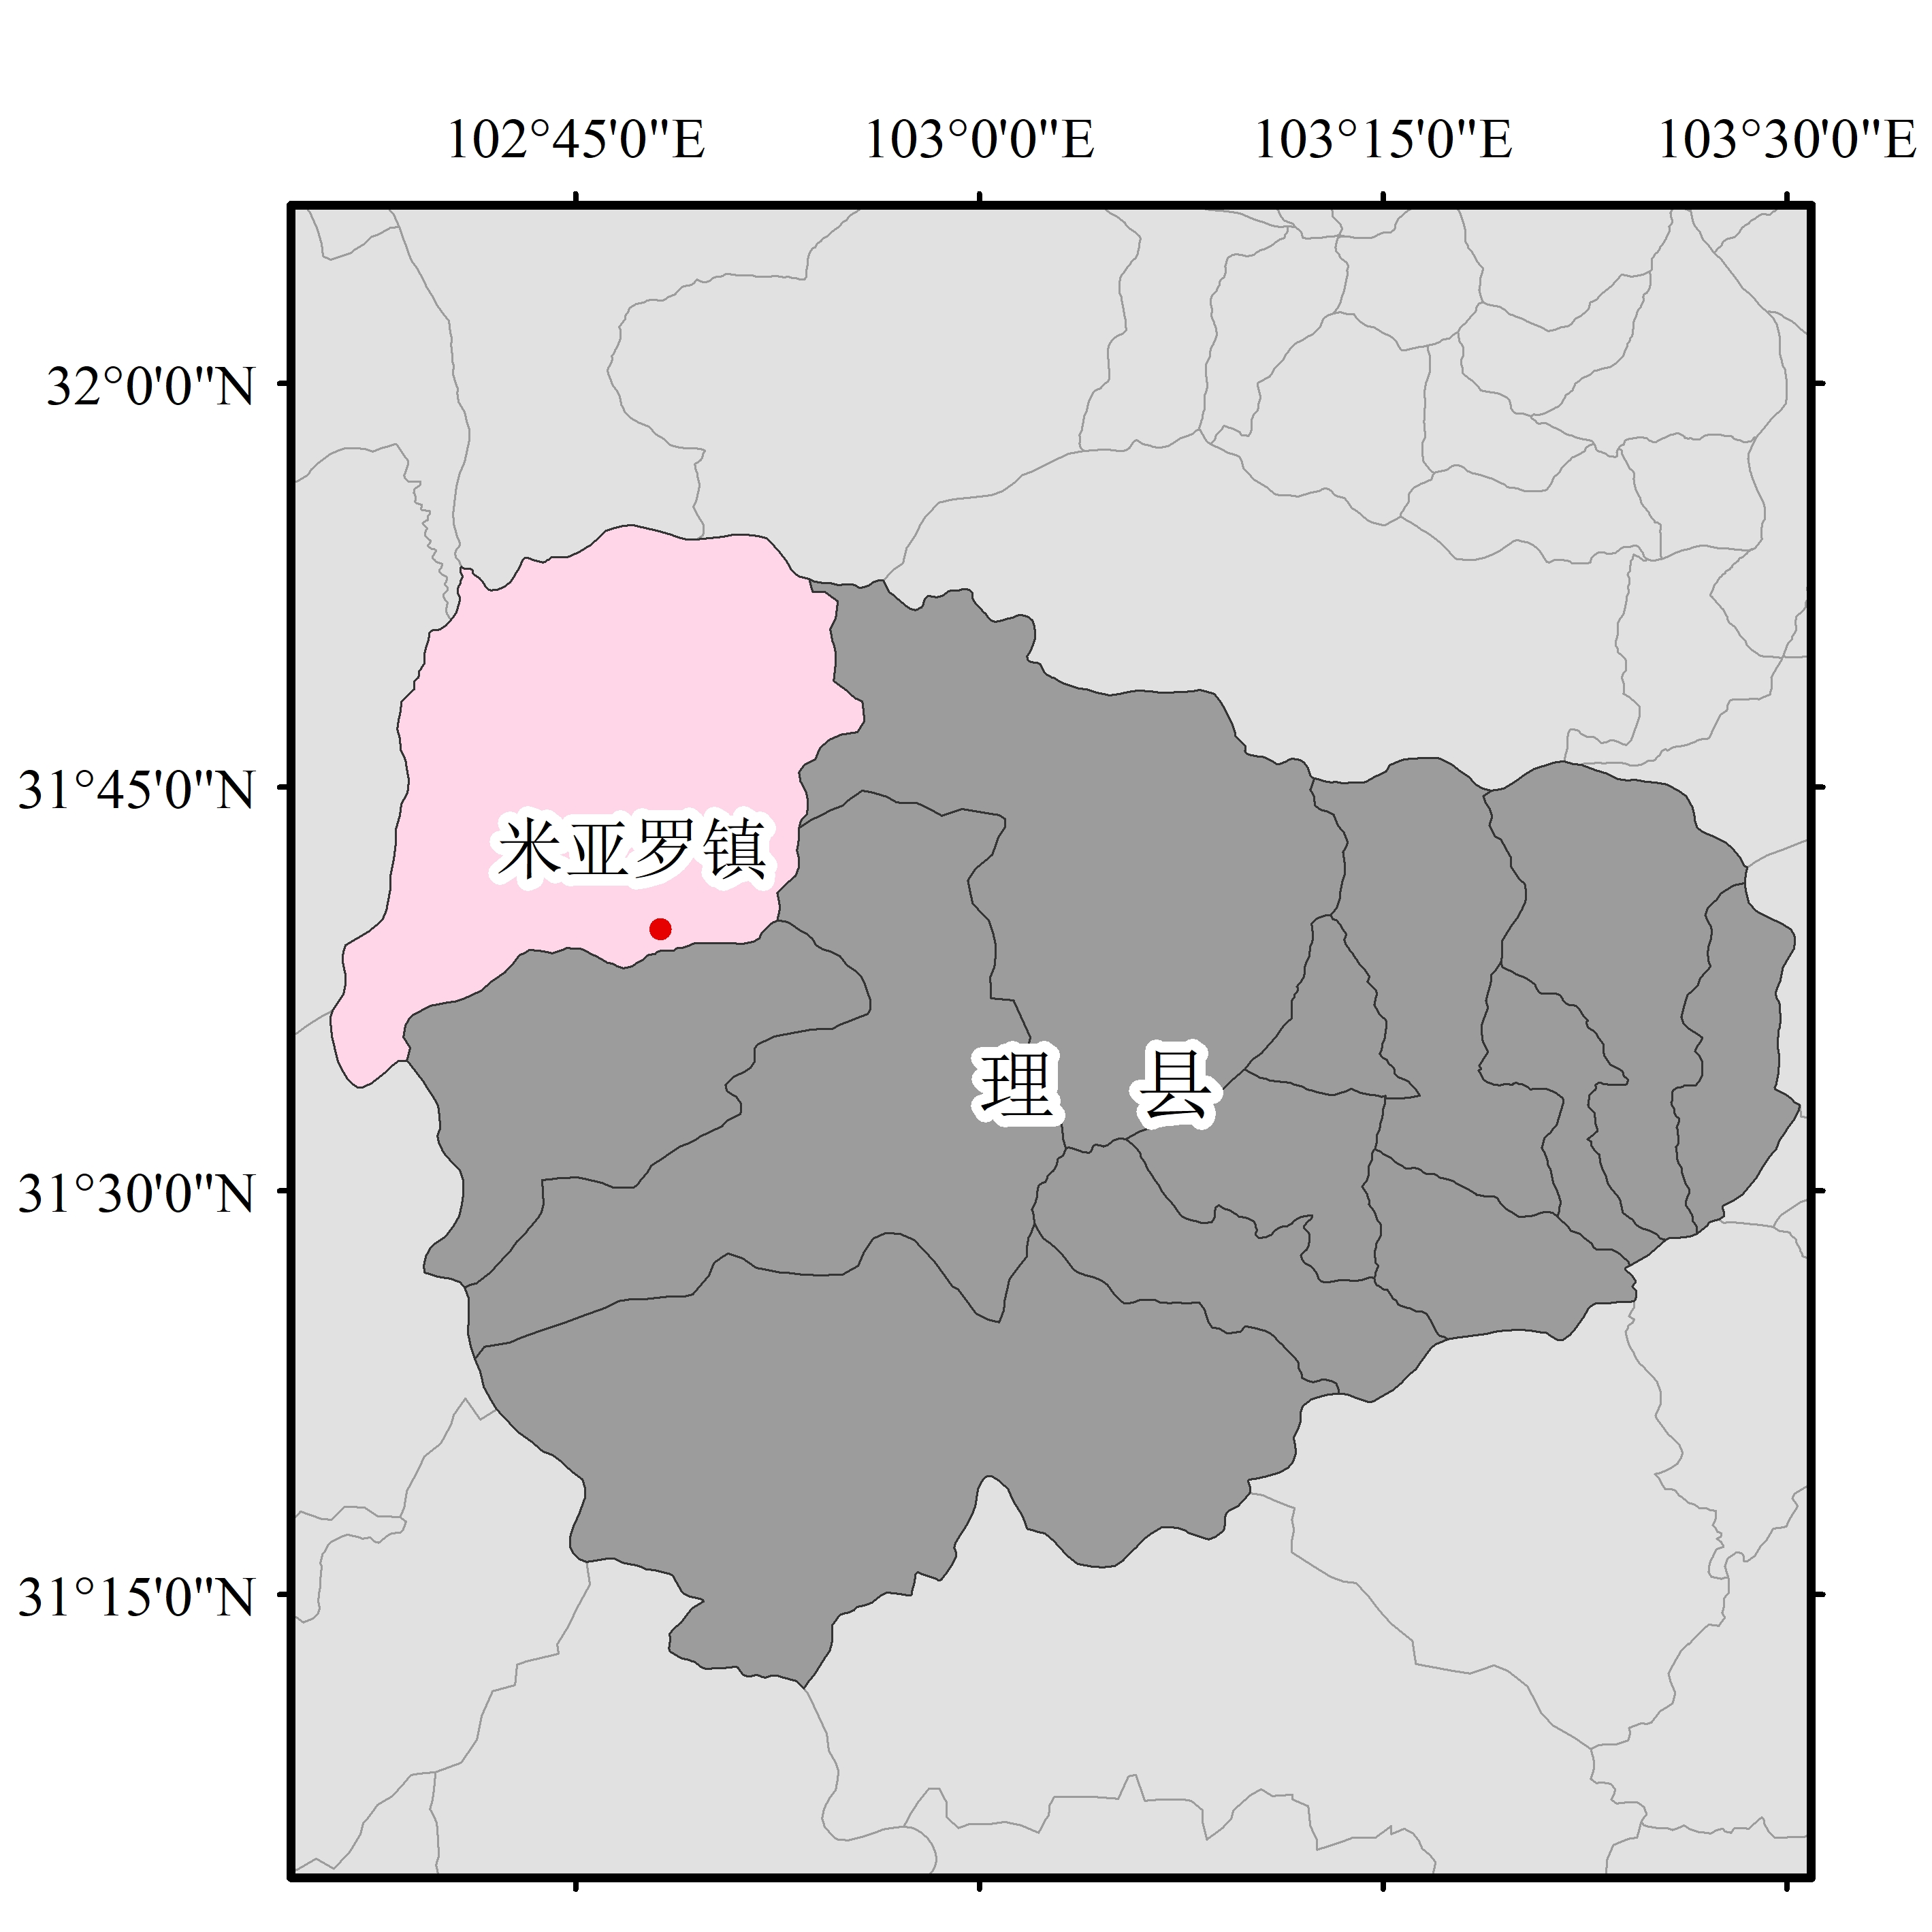
\includegraphics[width=0.8\textwidth]{img/LisCo.jpg}
\caption{米亚罗镇地理位置}
\label{myaglo}
\end{figure}

米亚罗镇位于理县西北部。唐贞观八年（634年）设北思县，治所北思城，即今米亚罗镇。后更名云山县。唐广德元年（763年）被吐蕃王国占领\cite[970-971]{xingzheng-2012}。清代，米亚罗镇为梭磨土司（\tib{སོ་མང།}）辖区，称为“柯宋（或扣苏）上四沟”\cite[79]{<<Li-Xian-Zhi->>-Bian-Zuan-Wei-Yuan-Hui-1997-gj}。梭磨土司，即“四土嘉绒语”之名中“四土”所代指的四个土司（卓克基土司、梭磨土司、松岗土司、党坝土司）之一\cite{sun2000parallelisms}。1928年将“柯宋（扣苏）”改为“来苏”，1951年设上来苏区自治政府，1954年设米亚罗区人民政府，1955年设米亚罗镇\cite[79]{<<Li-Xian-Zhi->>-Bian-Zuan-Wei-Yuan-Hui-1997-gj}。目前，米亚罗镇下辖一个社区和九个村：红叶社区、米亚罗村、胆杆村、斯博果村、八角碉村、大郎坝村、夹壁村、二古溪村、猛古村、吉柯村。

\begin{figure}[H]
\centering
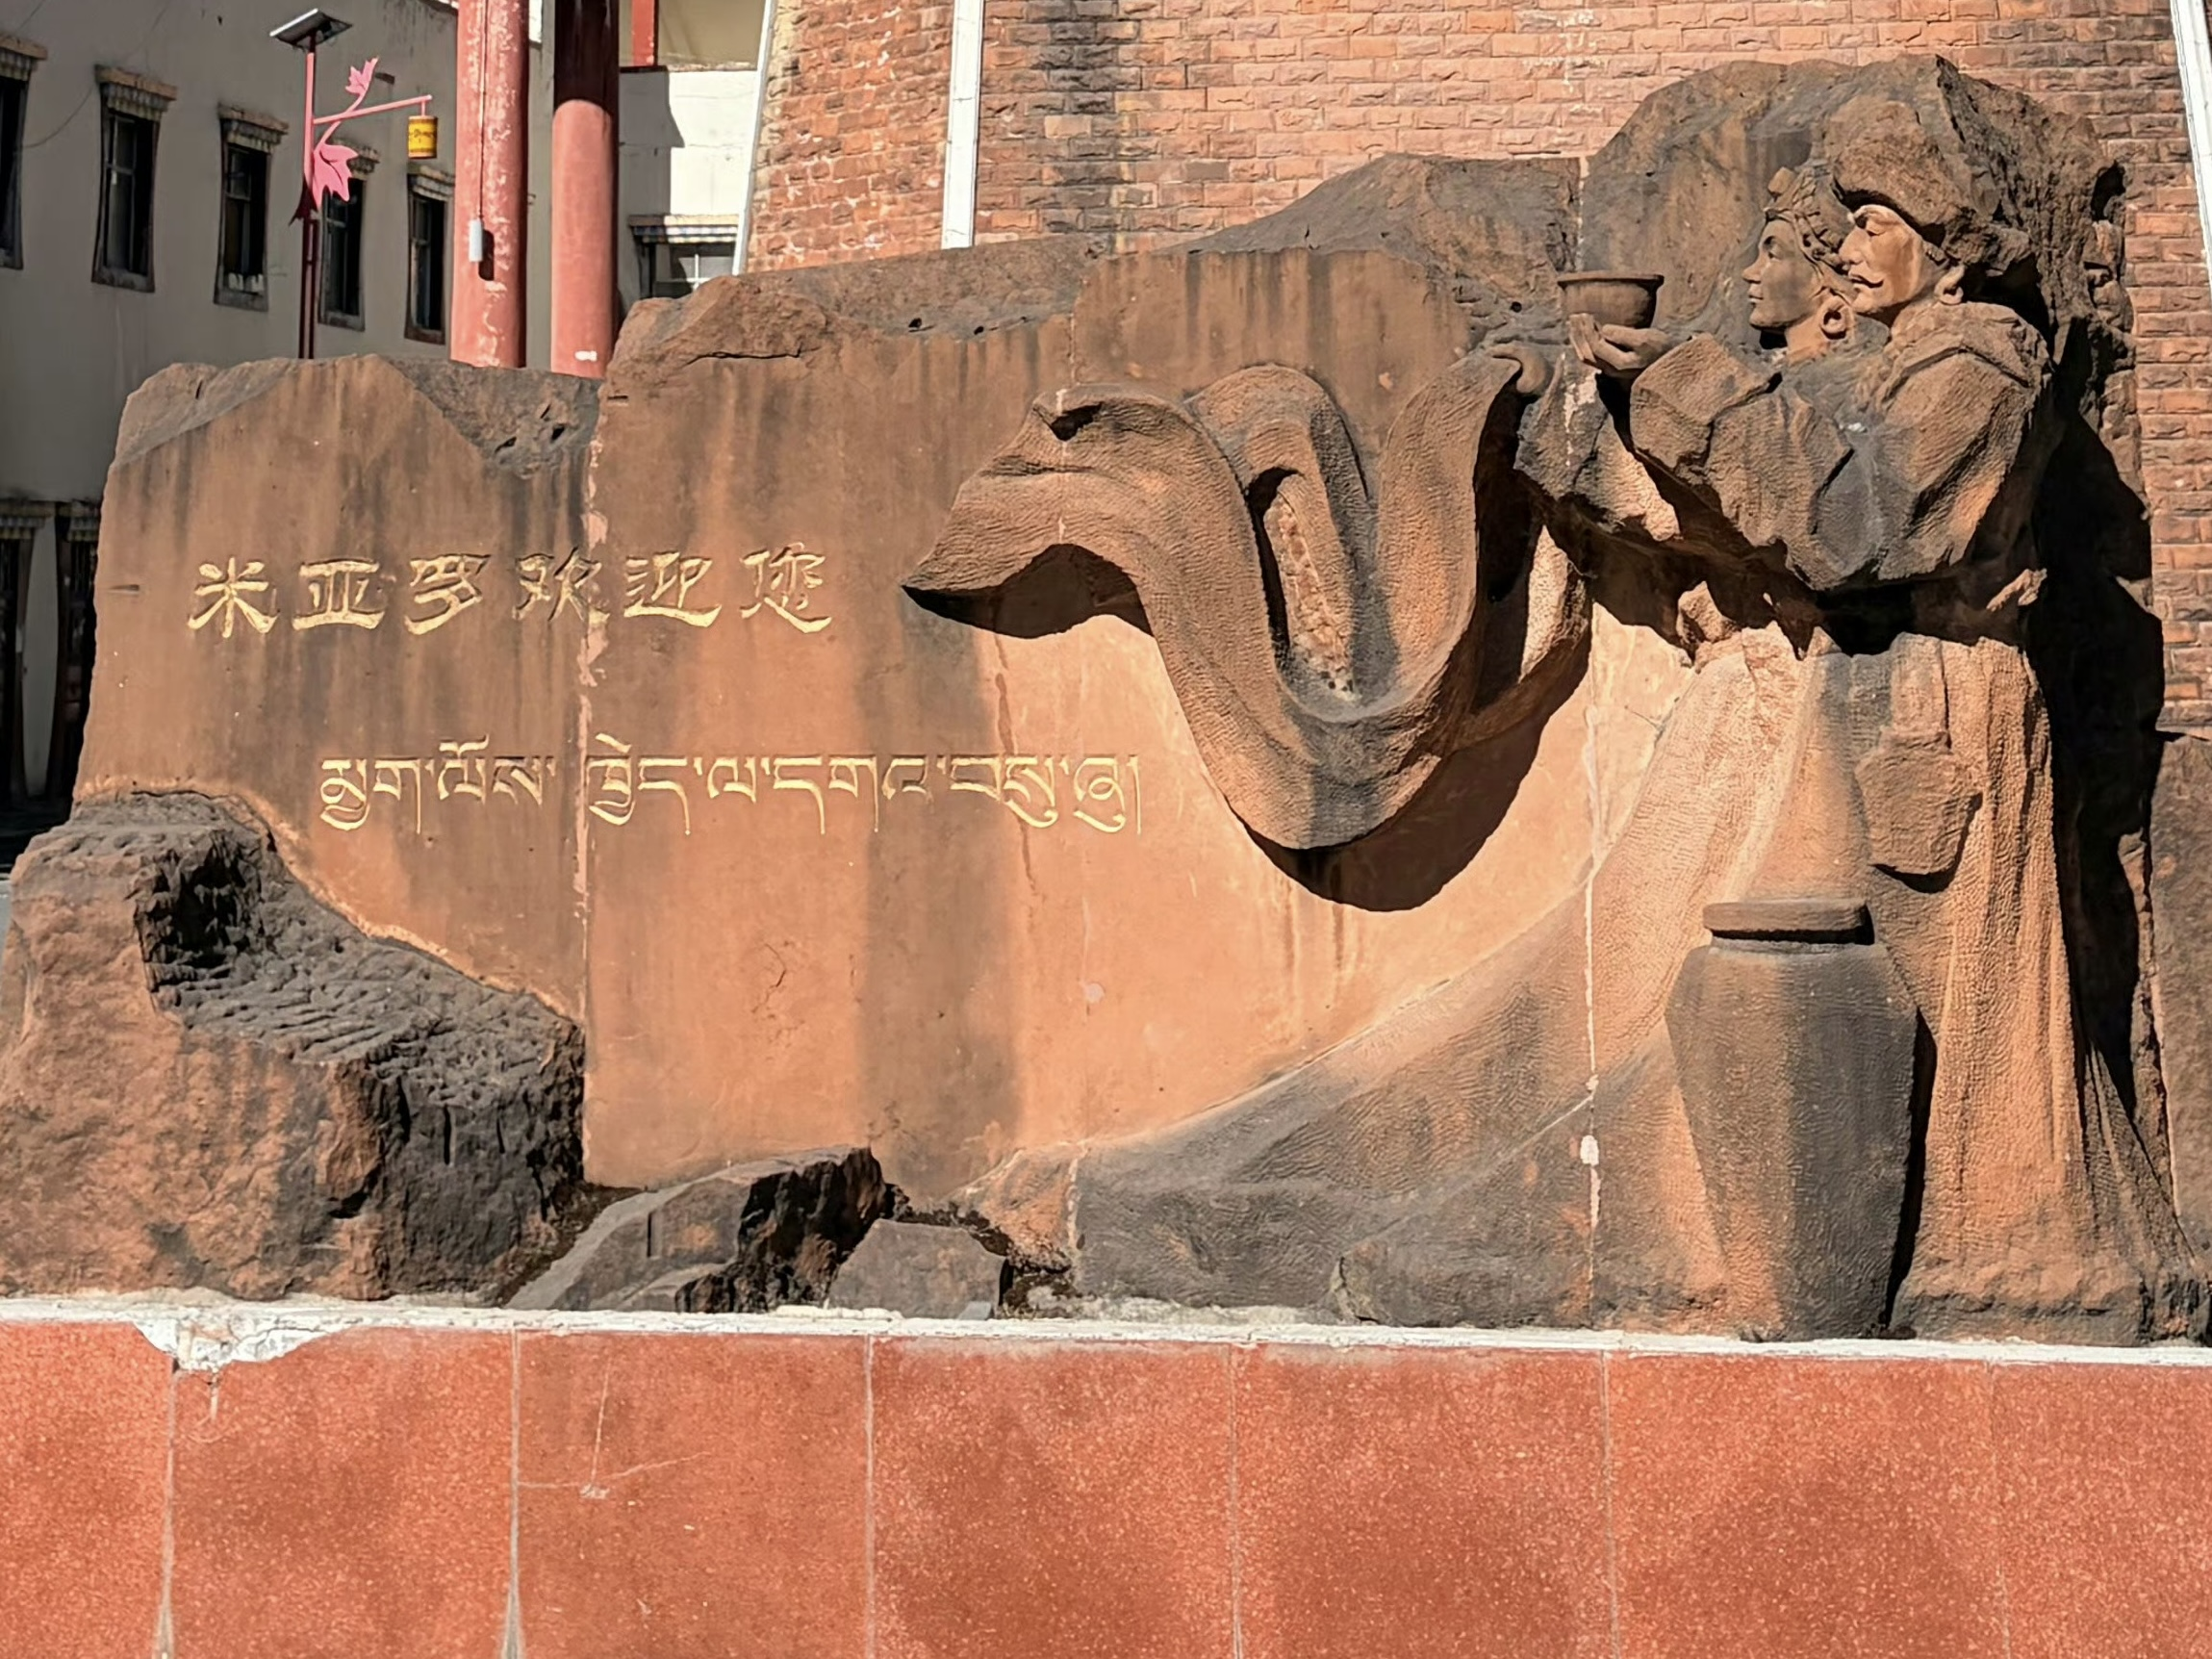
\includegraphics[width=0.8\textwidth]{img/miyaluo-pic2.jpg}
\caption{米亚罗（\tib{མྱག་ལོ།}）藏文转写}
\label{myaglopic}
\end{figure}

根据国家的民族识别工作，米亚罗镇的大多数四土嘉绒语母语者被识别为藏族。他们多数信仰藏传佛教宁玛派，不考虑语言因素，在生活习惯、文化上都接近藏族，自我认同也是藏族。除了藏族之外，米亚罗镇还存在部分汉族常住人口；作为旅游景区，米亚罗镇还有大量来自各地的游客。因而，米亚罗镇的四土嘉绒语主要和汉语普通话、西南官话存在接触，居民普遍存在四土嘉绒语和汉语的双语现象。此外，部分村落和寺庙也存在与藏语安多话（“草地话”）之间的接触。

现今，米亚罗镇的四土嘉绒语在各代人中均有保留。然而，虽然年轻一代的母语大多还是四土嘉绒语，但日常生活中的使用已大幅减少。在米亚罗镇及其下辖各村，大约有3000人正在使用四土嘉绒语米亚罗话。

\section{研究综述}

四土嘉绒语是汉藏语系嘉绒语组的一门独立语言，米亚罗话是四土嘉绒语的一个方言。

现代语言学意义上的“嘉绒语组”概念，最早由台湾语言学家孙天心提出。\textcite{sun2000parallelisms,sun2000stem}将当时的嘉绒语、霍尔巴—上寨语、拉坞戎语归类为藏缅语族羌语支内的一个独立语言支系。其中，“嘉绒语”下包括了四土话、茶堡话、四大坝话三个变体。向柏霖根据互通度将四大坝话拆分为草登话和日部话，认为“嘉绒语”有四土话、茶堡话、草登话、日部话四个方言\cite{Xiang2008,jacques2004phonologie}。近期的分类将嘉绒语组划分为东部嘉绒语组（也称核心嘉绒语组，包括四土嘉绒语、茶堡嘉绒语、草登嘉绒语、日部嘉绒语）和西部嘉绒语组（包括道孚语、绰斯甲语、西夏语）两支\cite{lai2020tangut}，分类树如下：

\begin{center}
    \begin{tikzpicture}
        \Tree
        [.嘉绒语组 
            [.东部嘉绒语组 
                [.四土嘉绒语 ]
                [.茶堡嘉绒语 ]
                [.草登嘉绒语 ]
                [.日部嘉绒语 ]
             ]
            [.西部嘉绒语组 
                [.道孚语 ]
                [.绰斯甲语 ]
                [.西夏语 ]
            ]
        ]
    \end{tikzpicture}
\end{center}

其中，四土嘉绒语是使用最广泛的嘉绒语组语言，分布在阿坝州的马尔康市、金川县、小金县、黑水县、理县、红原县、汶川县，以及甘孜州的丹巴县和雅安市的宝兴县\cite[411]{Lin-1993-cd}。四土嘉绒语同样是最早被记录的嘉绒语组语言。最早的文献记载是清代乾隆十五年（1750年）成书的《西蕃译语》，其中的《嘉绒译语》记载了740条四土嘉绒语词汇，采用藏文字母和汉字记音\cite{Gong2018-aw,Nie2010}。学术性报告则可追溯至19世纪末\cite{Von_Rosthorn1897-du}。早期的描写性著作包括\textcite{Jin1949-uh}对理县杂谷脑镇方言的研究，以及\textcite{Jin-1957-oe}对梭磨话的研究。随后，马尔康卓克基镇的卓克基话成为语言学研究的焦点，\textcite{Lin-1993-cd}提供了全面的语法，\textcite{Lin-2016-dr}提供了标注文本，\textcite{hsieh1999theoretical,lin2012no}分析了其音系，\textcite{Lin2000-jd,Nagano1984-tn,Wei2001-mw}分析了其动词形态。近年来，学界出版了四土嘉绒语其他方言的一些重要参考语法，包括\textcite{zhang2016phonologie,Zhang2020-ya}关于白湾话的参考语法、\textcite{prins2011web}关于脚木足话的著作、\textcite{Chang-Ye-2018-gb}对莫拉话的研究。

\begin{figure}[H]
\centering
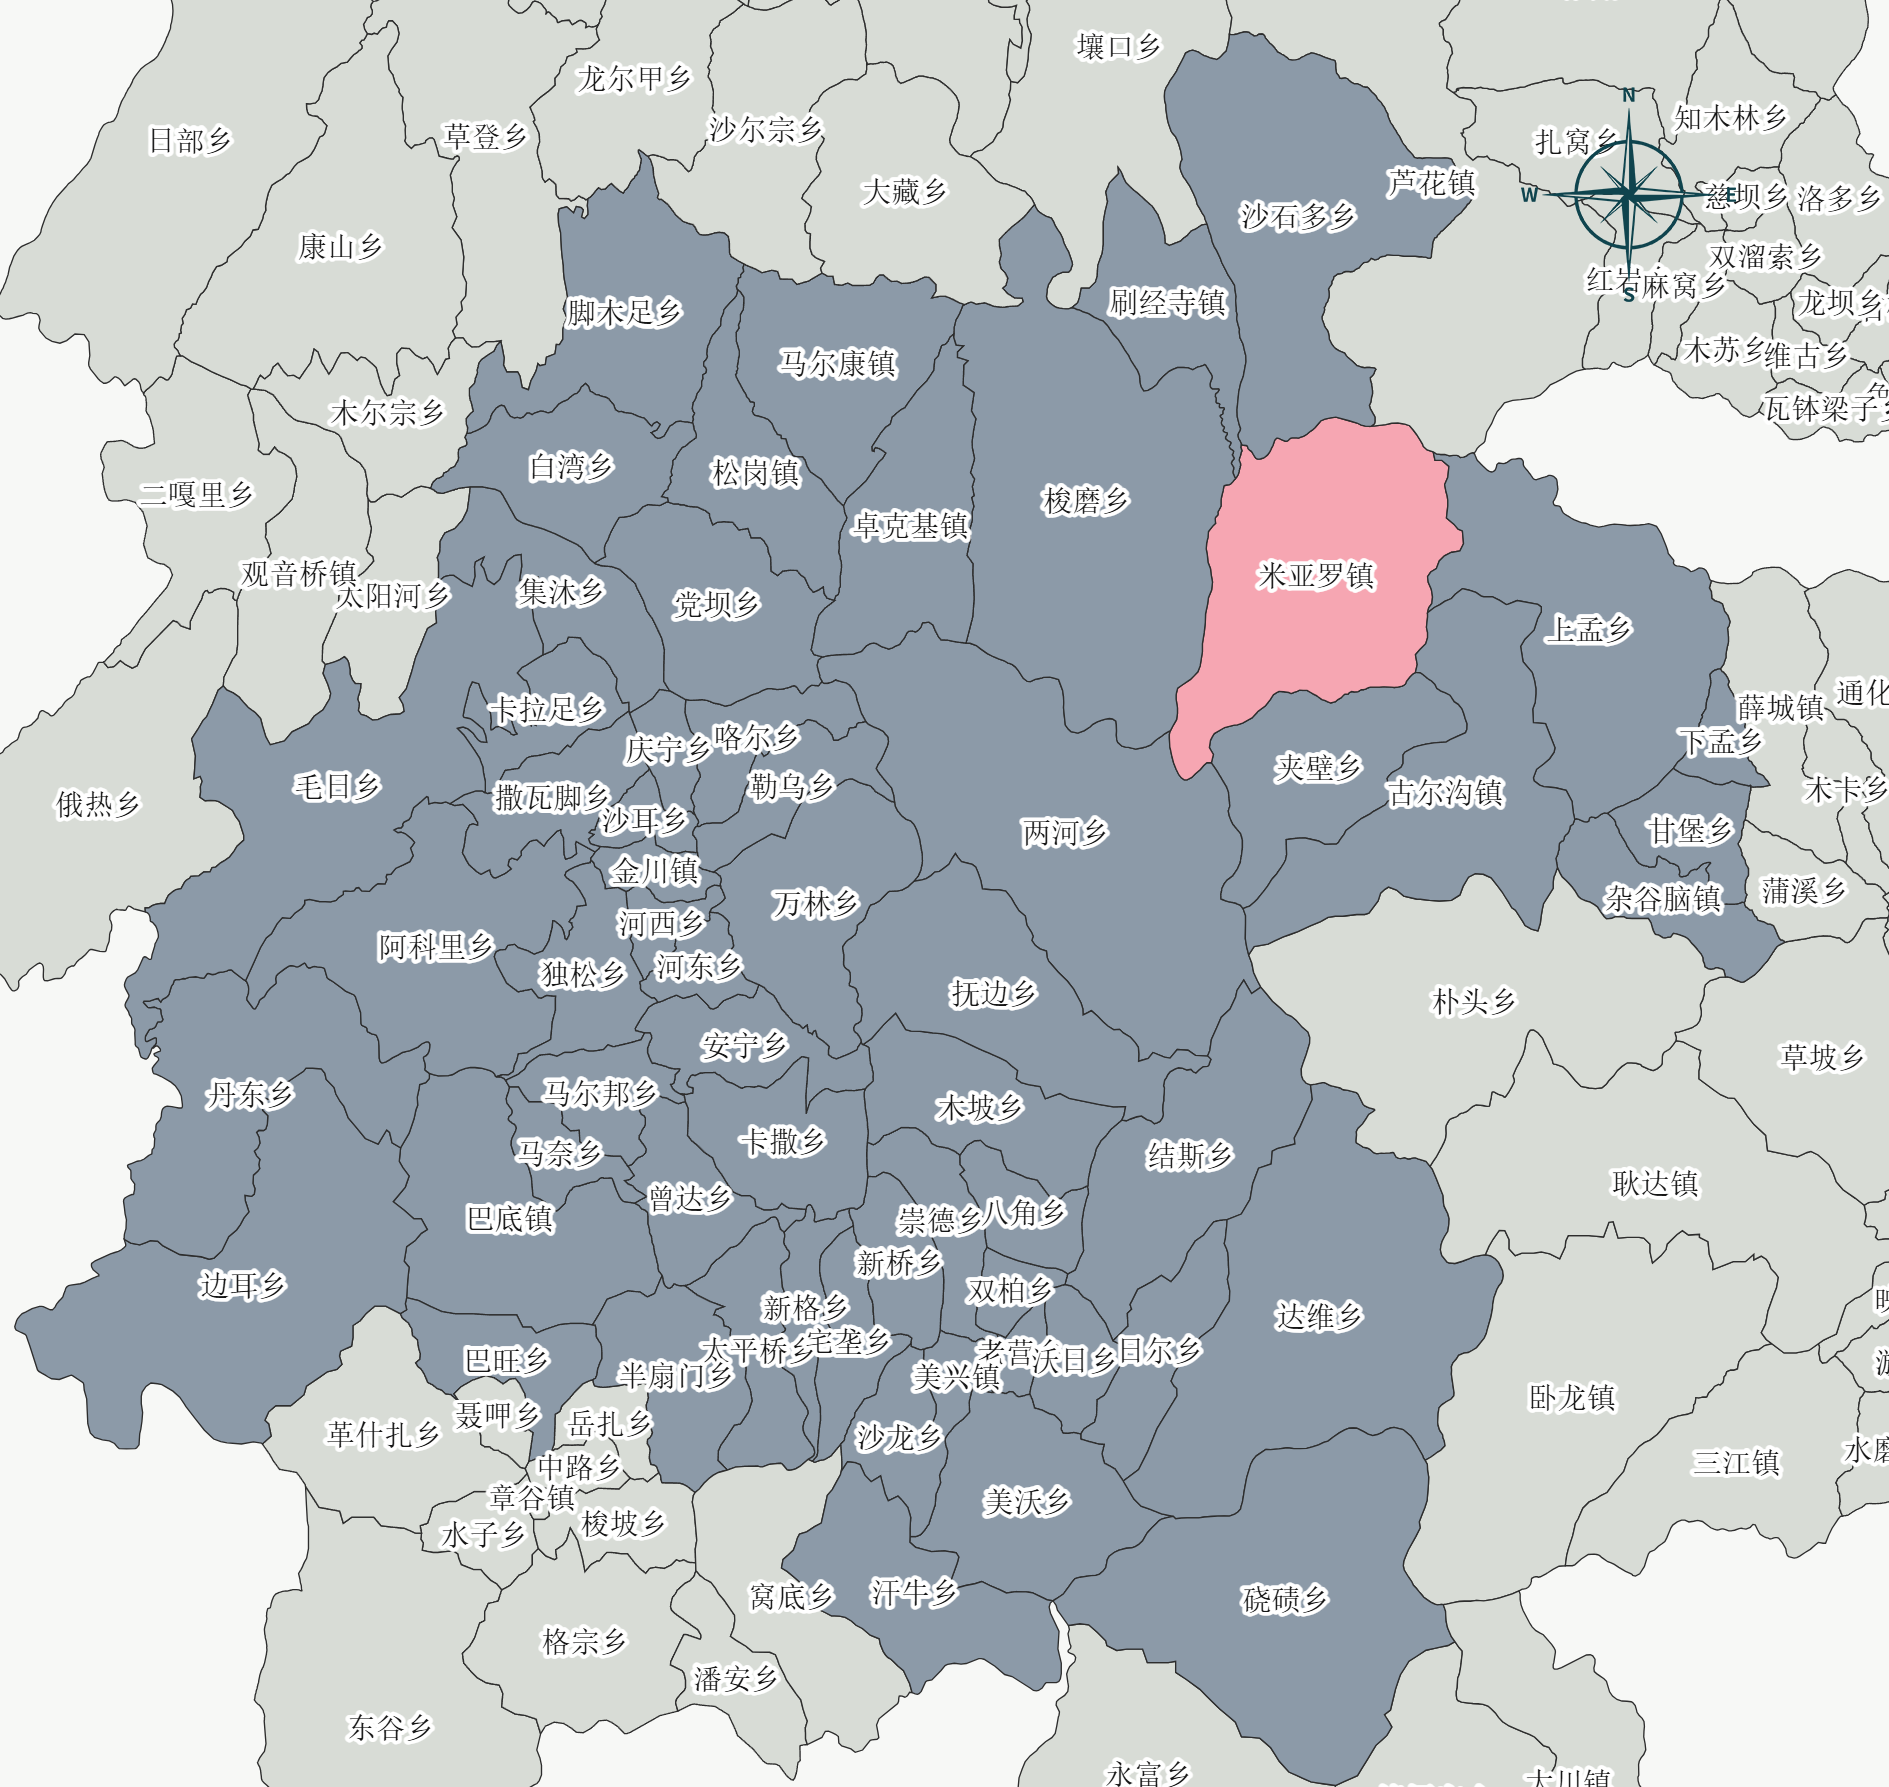
\includegraphics[width=0.8\textwidth]{img/situ.png}
\caption{四土嘉绒语的大致分布}
\label{situ-pic}
\end{figure}

本文所讨论的四土嘉绒语米亚罗话，是四土嘉绒语分布区域东南端的方言之一\cite[102-103]{gates2014situ}。根据\textcite{gates2014situ}的方言学研究，四土嘉绒语可分为中东部和南部方言区。米亚罗话正位于这两个区域的交界处，在民族语言认同和互通度上均表现出过渡性的特征。\textcite{Gong2018-aw}将四土嘉绒语内部方言粗略分为“去鼻冠音”（deprenasalization）类型和“弱化”（leniting）类型，而米亚罗话属于前者。然而，米亚罗话目前仍基本处于文献记录不足状态。现存唯一的记录是一份包含约200个句子和1200个词汇的简短调查，是\textcite{Nagano2013-hy}在嘉绒语组全域进行的大型调查项目的一部分；但这份记录缺乏语音或音系分析。本文将通过田野调查所得材料，首次系统分析四土嘉绒语米亚罗话的音系。

\section{田野工作与语料}

本文的记录对象主要是米亚罗话在理县米亚罗镇的变体。本文的描写基于作者自2025年以来的三次田野调查（2025.1-2、4-5、8-9月）。调查内容包括：对词表进行诱导式调查和录音\footnote{词表参考\textcite{Huang1992,Xiang2008,Lin-2016-dr}进行编制。}、录制故事和对话等长篇语料。除了线下的田野调查，还通过电话、微信等手段与发音人保持联系。本文基于的录音音频数据均为线下录音，录音在安静的室内进行，录音设备为TASCAM DR100mk3录音笔，音频采样率为48 kHz，采样精度为24-bit，保存为立体声WAV格式。录音后的音频文件在Adobe Audition软件中进行剪辑与整理，未进行任何降噪滤波处理。

本文的大部分记音、录音数据及音系分析，均基于主要发音人翁真卓玛（\tib{དབང་འཛིན་སྒྲོལ་མ།}）。发音人出生于1974年，自幼生活在米亚罗镇，现于当地经营一家民宿。其母语为四土嘉绒语米亚罗话，并能流利使用汉语西南官话。此外，她还曾在汶川县就读中专，并学习过一段时间英语。

此外，本文的部分数据有赖于其他发音人。斯玛朗（男，1967年出生）是米亚罗镇米亚罗村的一名猎户，为本文提供了部分动物、植物词汇数据；阿让（男，1938年出生）是米亚罗镇斯博果村的一名农户，为本文提供了部分长语料数据和词汇数据。

本文的记音主要采用国际语音学学会发布的国际音标系统；在此基础上，使用了汉藏语语言学界常使用的/ɿ/标记舌尖前不圆唇元音，相当于国际音标的/ɹ̩/。对于声调，基于四土嘉绒语米亚罗话的词调模式和底层的缺性声调对立（详见第\ref{chaptertone}章），本文在记音中采用两种方式：词末音节韵核为V，或词末标“1”表示“1调”即底层零声调；词末音节韵核为V̂，或词末标“2”表示“2调”即底层降调。

目前，本文涉及的所有词汇的记音和音频数据均已被整理好，并收录、公开在作者开发的嘉绒语词表数据库中，可通过\url{https://flagrain.cn/rgyalrong/}访问。本文涉及的诱导式调查和自然语料的句子音频也已被切分好，可以通过电子邮件me@flagrain.cn向作者取得。

对于文内音频和文本数据的处理，本文均采用作者独立编写的Python程序进行；尤其地，对音频的声学分析采用了Praat的Python接口Parselmouth \parencite{jadoul2018parselmouth,boersma2026praat}。
\chapter{音节结构}

本文拟将米亚罗话的音节分析为如下结构：

\begin{center}
    \begin{tikzpicture}
        \Tree
        [.音节
            [.（声母） 
                [.（冠音） ]
                [.（首位） ]
                [.（中间位） ]
             ]
            [.韵基
                [.韵核 ]
                [.（韵尾） ]
             ]
        ]
    \end{tikzpicture}
\end{center}

\noindent
其中，声母和韵尾均可不出现。音节结构模式为(C$_{1}$)(C$_{2}$)(C$_{3}$)V(C$_{4}$)(C$_{5}$)：元音（即韵核（nucleus））前最多允许三个辅音（即声母（onset），其中C$_{1}$为冠音（preinitial）、C$_{2}$为首位（initial）、C$_{3}$为中间位（medial））、元音后最多允许两个辅音（即韵尾（coda））。最复杂的音节结构为CCCVCC，例如 /zɡroks/ “手镯”。

\begin{center}
    \begin{tikzpicture}
        \Tree
        [.音节
            [.声母 
                [.冠音 z ]
                [.首位 ɡ ]
                [.中间位 r ]
             ]
            [.韵基
                [.韵核 o ]
                [.韵尾 ks ]
            ]
        ]
    \end{tikzpicture}
\end{center}

\noindent
正如\textcite[47]{jacques2021grammar}对茶堡嘉绒语的判断，因为复杂的辅音簇，米亚罗话也不可能列出所有可能的音节。因此本文的分析同样只会分别分析声母和韵母。

\section{部分重叠} \label{reduplication}

嘉绒语组下许多语言中都存在部分重叠的现象，例如\textcite{jacques2021grammar}描写了在茶堡话的动词和部分名词中存在的部分重叠，分为声母重叠和韵母重叠，其中声母重叠的构造方式是在原音节前插入一个滋生音节；\textcite{lai2017grammaire}在俄热话中观察到的部分重叠构造则是滋生音节作为后缀附着在原音节，即词的最后一个音节之后。

米亚罗话中观察到的部分重叠现象在构造上与茶堡话的声母重叠相似，都是将滋生音节插入到原音节之前。米亚罗话的部分重叠指的是照原样复制单音节并改变其韵母部分的音系过程。具体构造方式为：对于词的最后一个音节$\sigma$，删除其韵尾部分形成滋生音节$\sigma'$，再将$\sigma'$插入到$\sigma$之前，形成新的音节序列$\sigma'\sigma$。例如：

\begin{exe}
\ex kəmbrô “高的” $\rightarrow$ kəmbrombrô \\
\gll kə- mbro- mbrô \\
     $\sigma_{1}$ $\sigma_{2}'$ $\sigma_{2}$ \\
\end{exe}

\begin{exe}
\ex kənpjôk “软的” $\rightarrow$ kənpjonpjôk \\
\gll kə- npjo- npjôk \\
     $\sigma_{1}$ $\sigma_{2}'$ $\sigma_{2}$ \\
\end{exe}

米亚罗话的部分重叠在形容词中相当能产，即使是在借词中也能应用。例如[kə-xɐw]“好的”就有重叠形式[kə-xɐ-xɐ̂w]。形容词之外，部分名词，尤其是一些方位、时间名词和量词也存在部分重叠现象。动词可以观察到一些部分重叠的形式，但其已经相当词汇化，例如[kɐ-nɐ-wze-wzet]“犹豫”，其理论上对应的无重叠形式*[kɐ-nɐwzet]并不存在。

部分重叠因为会完整重复词末音节的声母部分，因此可以用来测试音节歧义（ambisyllabicity）。例如[kə-nejnə̂]“内向的”，虽然看似有[kə-ne.jnə̂]和[kə-nej.nə̂]两种音节划分方式，但观察其重叠形式[kə-ne-jnə-jnə̂]可以发现其最末音节的声母应当是/jn/，因此音节划分只能是[kə-ne.jnə̂]。
\chapter{声母}\label{charonset}

\section{辅音音位}

米亚罗话共有33个辅音音位，如表\ref{consonant}所示。

\begin{table}[H]
\vspace{5pt}
    \centering
    \caption{辅音音位}
    \label{consonant}
\begin{tabular}{cccccccc}
    
   \toprule
     & & 双唇 & 齿龈 & 龈后 & 龈-腭 & 硬腭 & 软腭 \\
   \midrule
   爆发音 & 清不送气 & /p/ & /t/ &  & & & /k/ \\
    & 清送气 & /pʰ/ & /tʰ/ &  & & & /kʰ/ \\
    & 浊不送气 & /b/ & /d/ &  & & & /ɡ/ \\
    鼻音 & & /m/ & /n/ &  & & /ɲ/ & /ŋ/ \\
    擦音 & 清 &  & /s/ & /ʃ/ & /ɕ/ & & /x/ \\
     & 浊 &  & /z/ & /ʒ/ & & &  \\
    塞擦音 & 清不送气 &  & /ts/ & /tʃ/ & /tɕ/ & &  \\
    & 清送气 &  & /tsʰ/ & /tʃʰ/ & /tɕʰ/ & &  \\
    & 浊不送气 & & /dz/ & /dʒ/ & /dʑ/ & &  \\
    颤音 & &  & /r/ &  &  & &  \\
    边擦音 & &  & /ɬ/ &  &  & &  \\
    边近音 & &  & /l/ &  &  & &  \\
    近音 & & /w/ &  &  &  & /j/ &  \\
   \bottomrule
\end{tabular}
\end{table}

表\ref{conex}列出了全部的单辅音声母示例。

\begin{table}[H]
\vspace{5pt}
    \centering
    \caption{辅音示例}
    \label{conex}
\begin{tabular}{ccc|ccc}
     \toprule
	/p/ & [kɐ-po] & “纺” & /l/ & [kə-lə] & “重的” \\
	/pʰ/ & [kɐ-pʰô] & “躲” & /ɬ/ & [ɬɐ̂] & “神” \\
	/b/ & [kə-bə̂s] & “灰暗的” & /ʃ/ & [kə-ʃək] & “新的” \\
	/m/ & [tɐ-mî] & “脚” & /tʃ/ & [kə-tʃən] & “短的” \\
	/w/ & [tə-wom] & “尸体” & /tʃʰ/ & [kɐ-tʃʰət] & “插” \\
	/t/ & [kɐ-tɐ̂] & “脱” & /dʒ/ & [tə-dʒɿ̂] & “皮肤” \\ 
	/tʰ/ & [tə-tʰɐ̂] & “书” & /ɕ/ & [tɐ-ɕet] & “梳子” \\ 
	/d/ & [tɐ-dok] & “毒药” & /tɕ/ & [kɐ-tɕet] & “关门” \\ 
	/n/ & [tə-nə] & “乳房” & /tɕʰ/ & [kɐ-tɕʰî] & “去” \\
	/s/ & [kɐ-sɐ̂r] & “娶” & /dʑ/ & [kʰə-dʑe] & “石杆菜（紫花碎米芥）” \\ 
	/z/ & [tə-zɐ̂] & “饭” & /ɲ/ & [ɲo] & “你们” \\ 
	/ts/ & [kə-tsə̂r] & “咸” & /j/ & [kɐ-jok] & “仰头” \\ 
	/tsʰ/ & [kə-tsʰɐr] & “闪光的” & /k/ & [tɐ-ku] & “头” \\ 
	/dz/ & [tə-mdzu] & “刺” & /kʰ/ & [kɐ-kʰo] & “晒” \\ 
	/r/ & [rowû] & “石头” & /ɡ/ & [tɐ-ɡɐm] & “蛋” \\ 
	/ʒ/ & [ʒowu] & “棉花” & /ŋ/ & [ŋos] & “是” \\ 
    /x/ & [kə-xɐw] & “好” &   &   &   \\
   \bottomrule
\end{tabular}
\end{table}

\subsection{爆发音}

米亚罗话的爆发音有清不送气、清送气、浊不送气三分对立，发声部位有双唇、齿龈、软腭。表\ref{ploex}列出了爆发音在元音/a/上的近似最小对。

\begin{table}[H]
\vspace{5pt}
    \centering
    \caption{爆发音的准最小对}
    \label{ploex}
\begin{tabular}{ccc}
   \toprule
    音位 & 例子 & 释义 \\
   \midrule
   /p/ & [tɐ-\textbf{pɐ̂}] & “父亲”  \\
   /pʰ/ & [\textbf{pʰɐ}tɐk] & “面条”  \\
   /b/ & [\textbf{bɐ}lə̂] & “没有角的牦牛”  \\
   /t/ & [kɐ-\textbf{tɐ̂}] & “放置”  \\
   /tʰ/ & [tə-\textbf{tʰɐ̂}] & “书”  \\
   /d/ & [tɐ-\textbf{dɐ}ste] & “火葬场”  \\
   /k/ & [\textbf{kɐ}-] & “动词词典形前缀” \\
   /kʰ/ & [\textbf{kʰɐ}lə̂] & “风” \\
   /ɡ/ & [tɐ-\textbf{ɡɐ}m] & “蛋” \\
   \bottomrule
\end{tabular}
\end{table}

其中齿龈爆发音/t/、/tʰ/、/d/在实际语音实现上更接近齿音[t̪]、[t̪ʰ]、[d̪]。

很多研究证明，爆发音的清浊对立不一定完全来自于发声起始时间（VOT）显示的带声性\cite{cho2019voice}；但通过测量米亚罗话的爆发音VOT，可以认为米亚罗话的清浊对立呈现出较为纯粹的带声性对立，见图\ref{votb}至\ref{votkh}，图中红线表示爆破释放，蓝线表示起声；浊不送气爆发音若在释放前已经出现周期性振动，则记为负值。测量结果见表\ref{plosivevot}。

\begin{figure}[H]
\centering
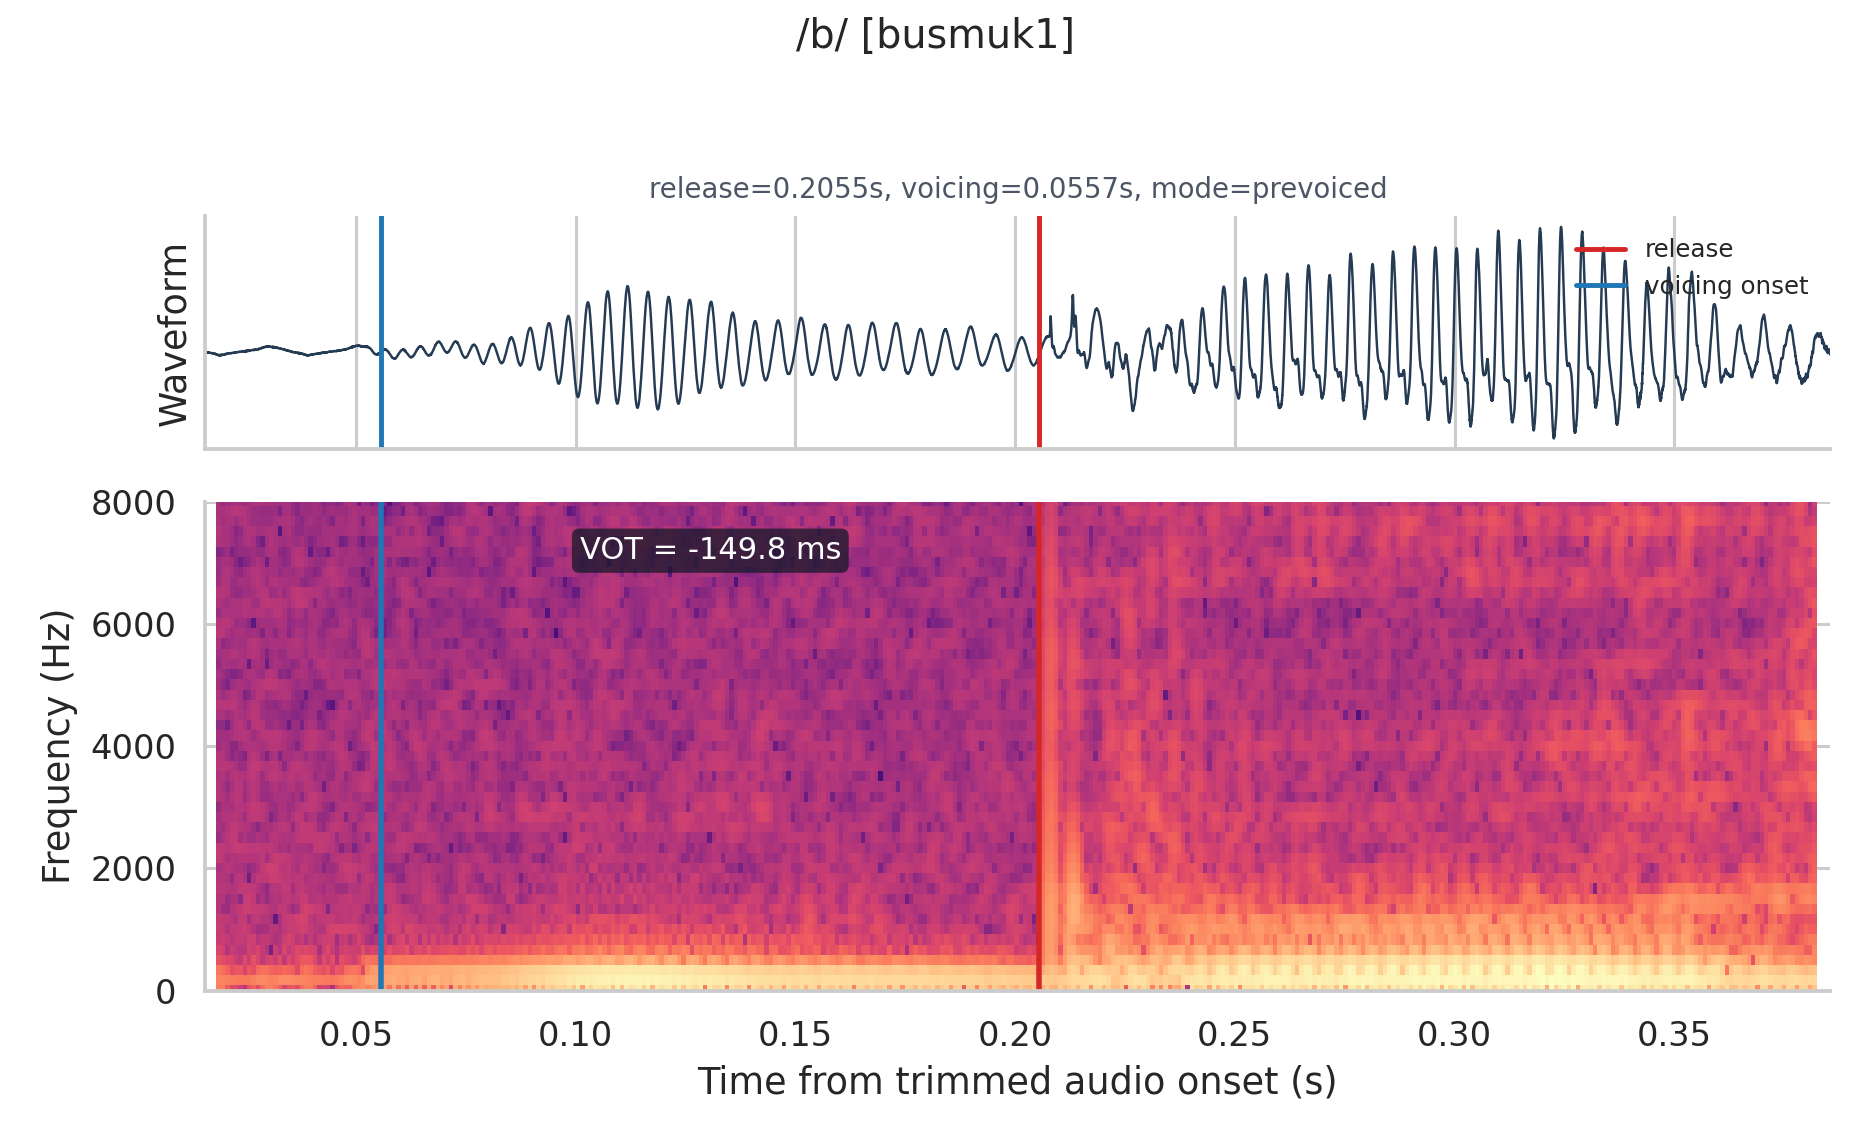
\includegraphics[width=0.8\textwidth]{img/vot_b.png}
\caption{[busmuk]“发霉”的发声起始时间}
\label{votb}
\end{figure}

\begin{figure}[H]
\centering
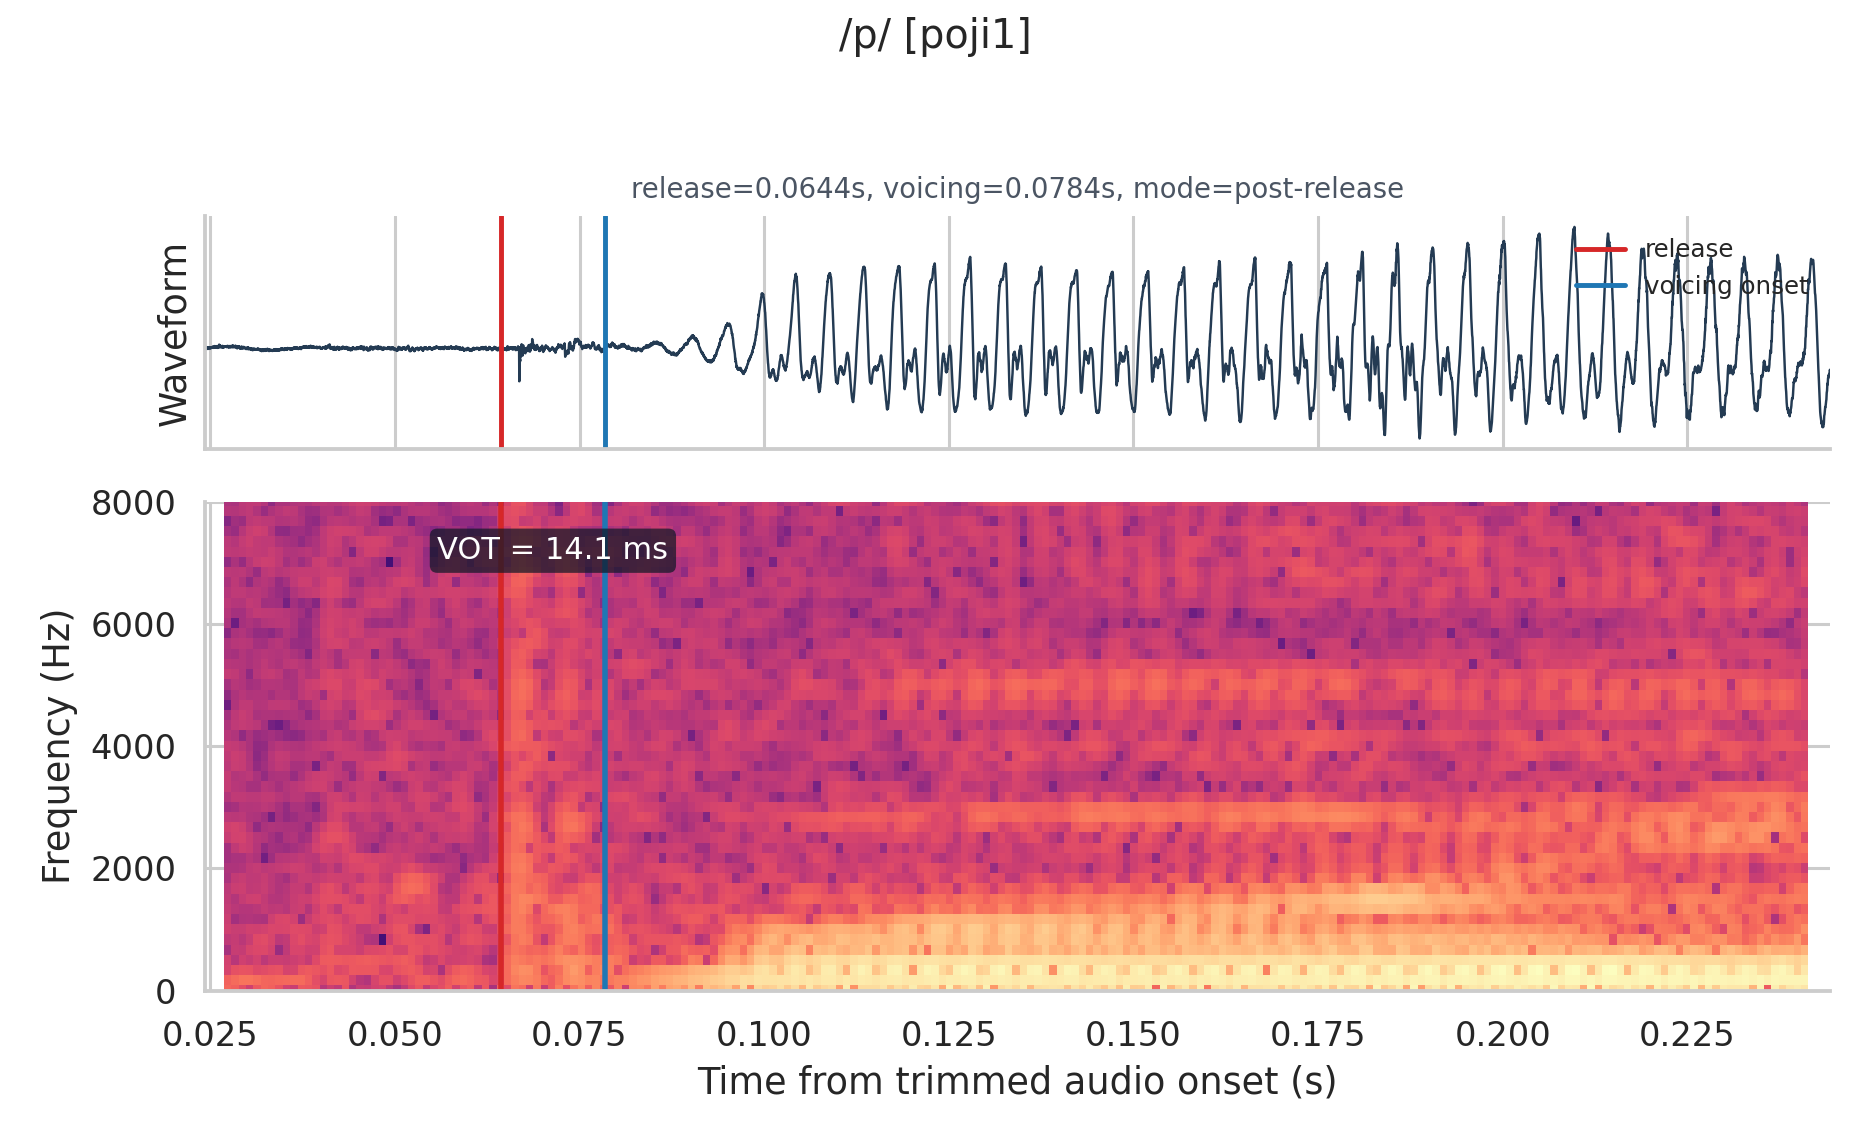
\includegraphics[width=0.8\textwidth]{img/vot_p.png}
\caption{[poji]“老鼠”的发声起始时间}
\label{votp}
\end{figure}

\begin{figure}[H]
\centering
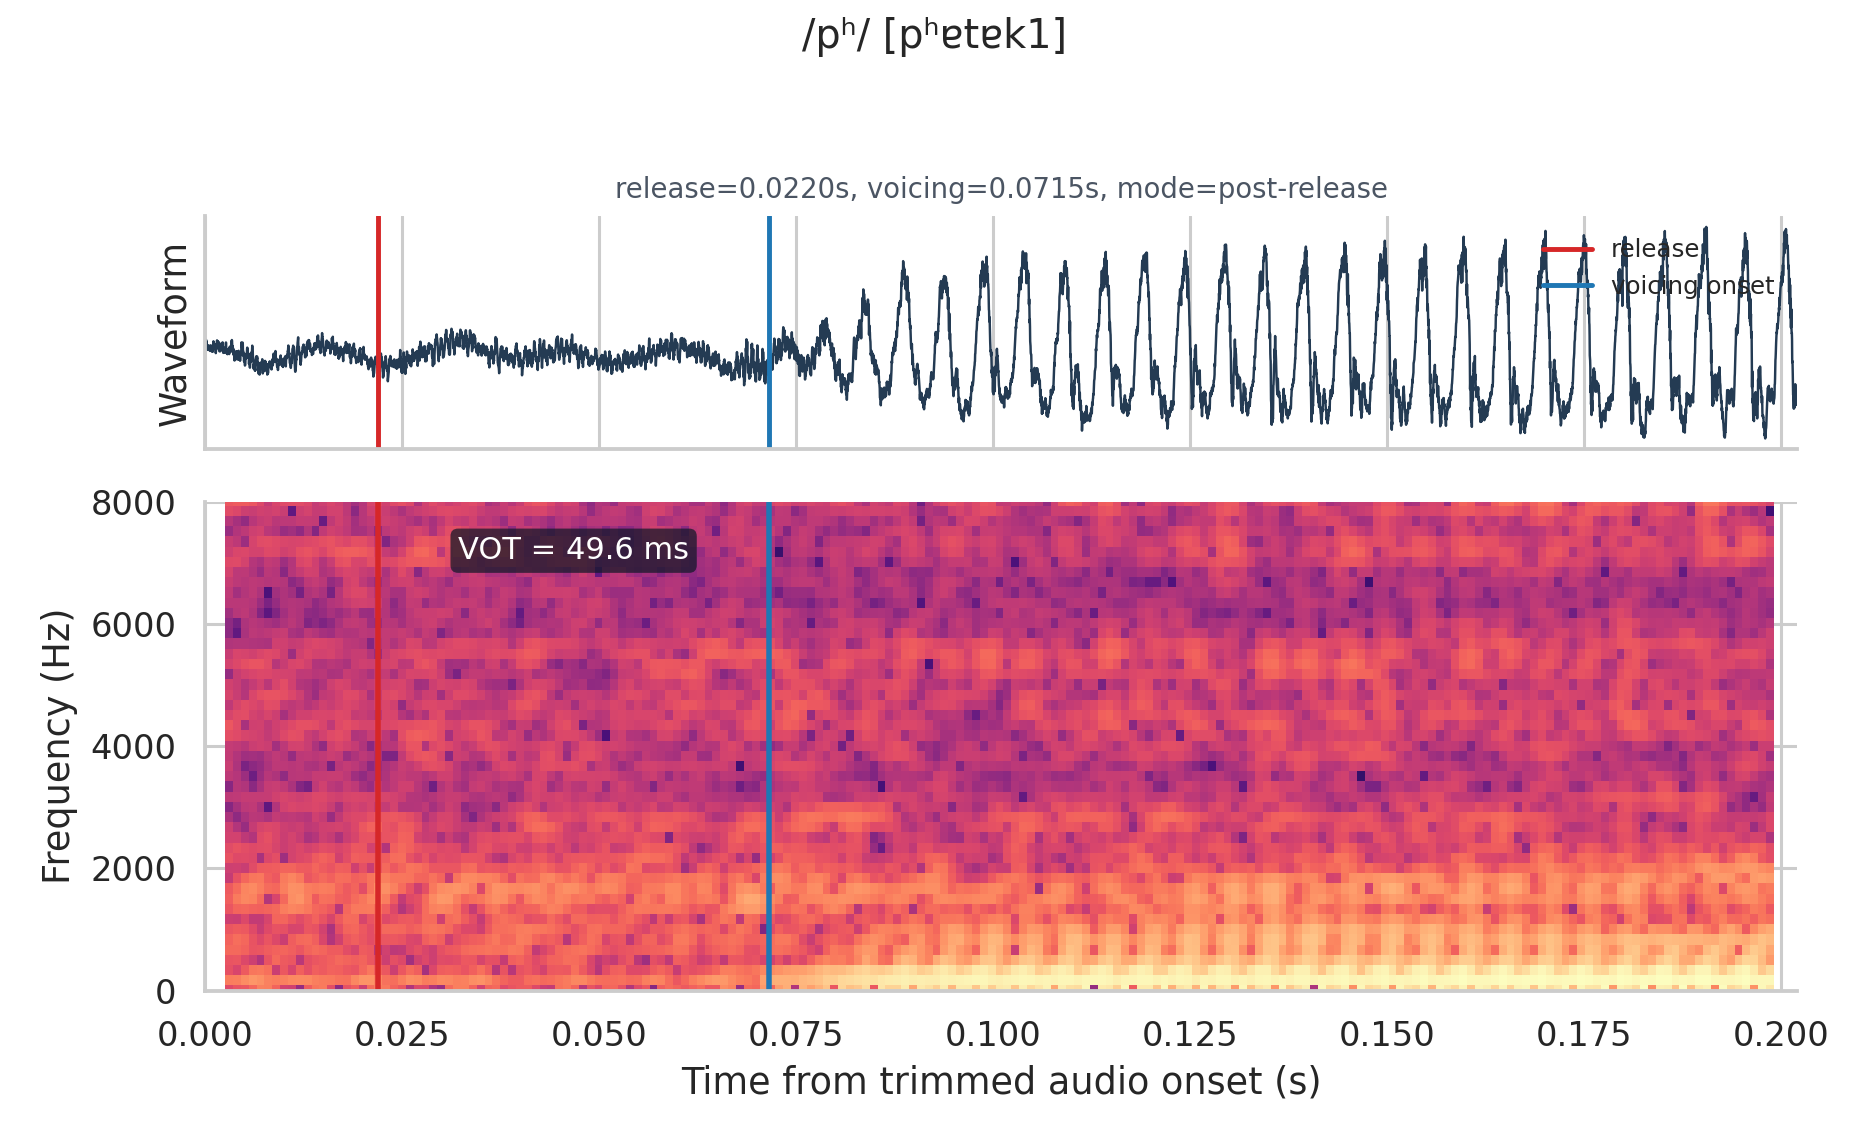
\includegraphics[width=0.8\textwidth]{img/vot_ph.png}
\caption{[pʰɐtɐk]“面条”的发声起始时间}
\label{votph}
\end{figure}

\begin{figure}[H]
\centering
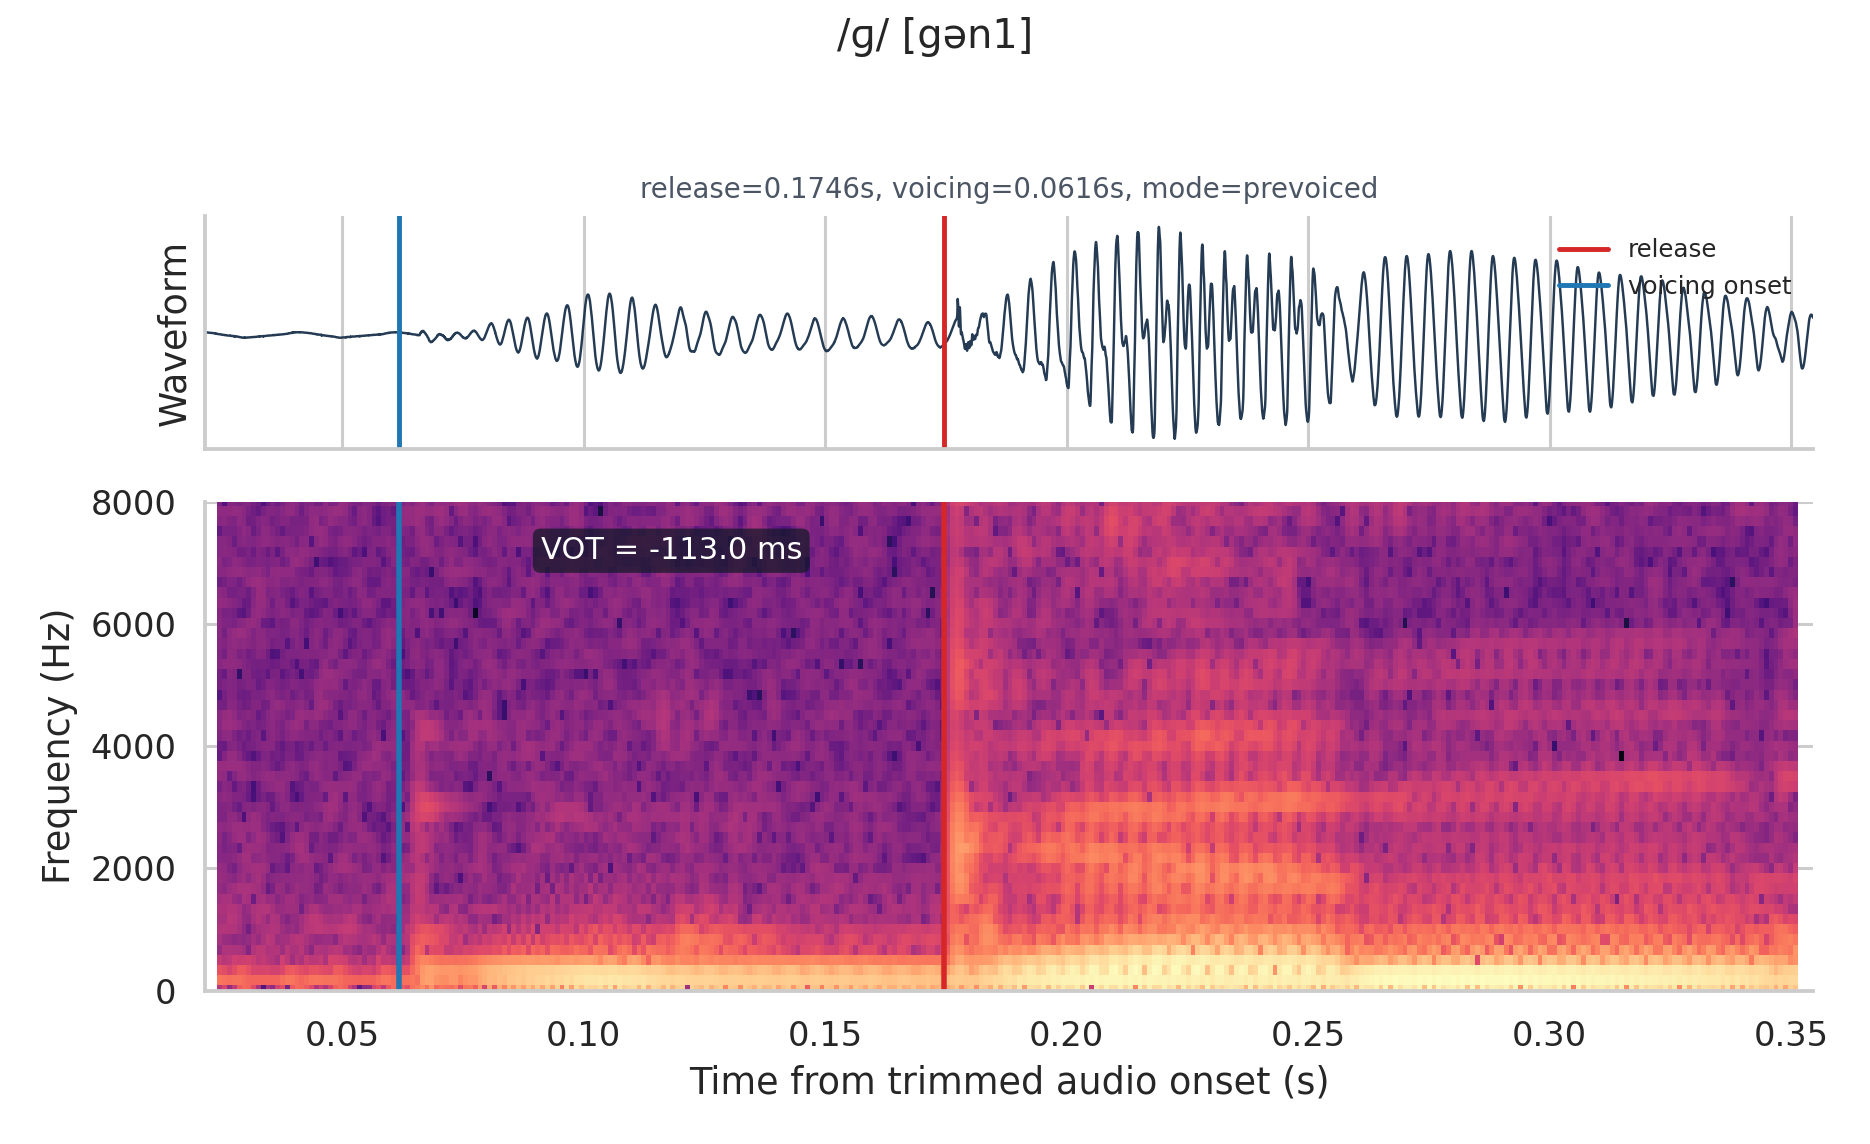
\includegraphics[width=0.8\textwidth]{img/vot_g.png}
\caption{[ɡən]“很”的发声起始时间}
\label{votg}
\end{figure}

\begin{figure}[H]
\centering
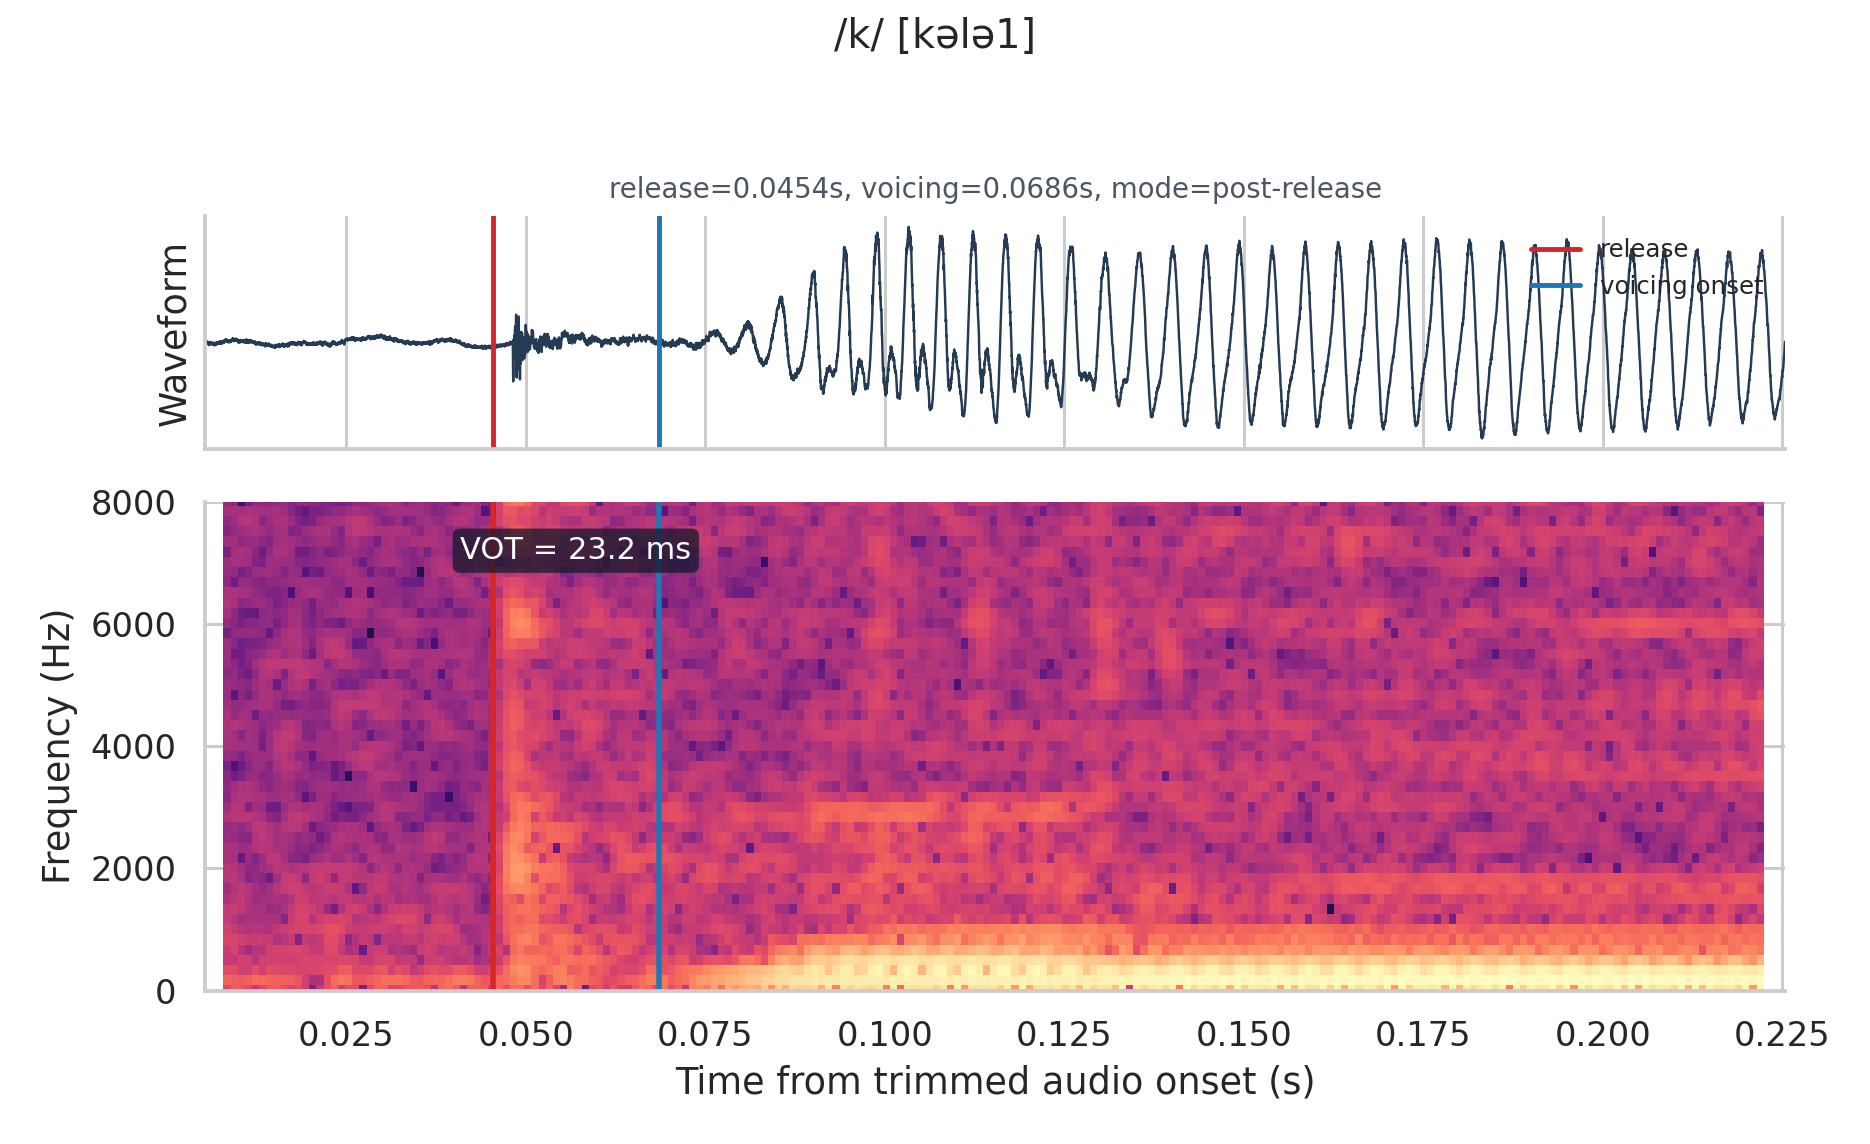
\includegraphics[width=0.8\textwidth]{img/vot_k.png}
\caption{[kələ]“虫子”的发声起始时间}
\label{votk}
\end{figure}

\begin{figure}[H]
\centering
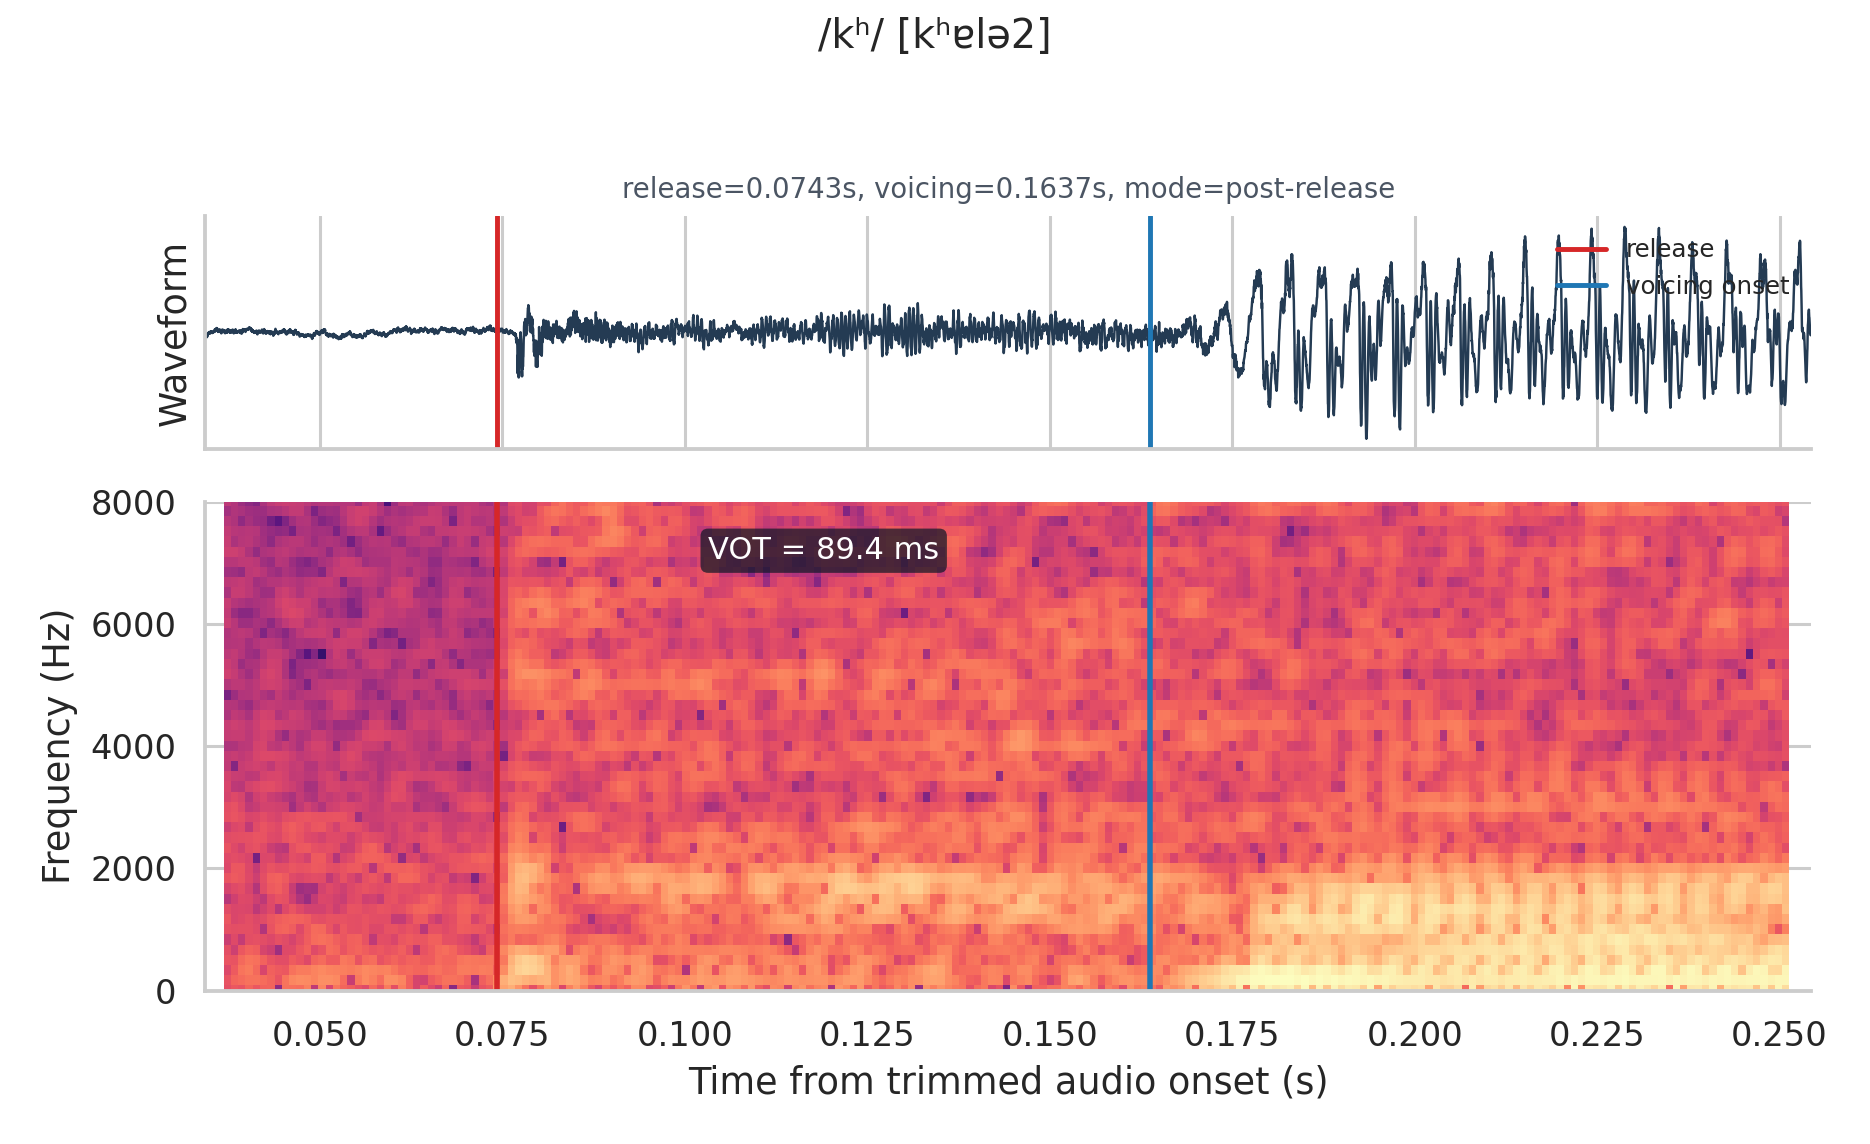
\includegraphics[width=0.8\textwidth]{img/vot_kh.png}
\caption{[kʰɐlə̂]“风”的发声起始时间}
\label{votkh}
\end{figure}

\begin{table}[H]
\vspace{5pt}
\centering
\caption{米亚罗话爆发音的VOT测量}
\label{plosivevot}
\small
\begin{tabular}{ccccc}
\toprule
发音部位 & 类型 & 音位 & 例词 & VOT(ms) \\
\midrule
双唇 & 清不送气 & /p/ & [poji] “老鼠” & +14.1 \\
双唇 & 清送气 & /pʰ/ & [pʰɐtɐk] “面条” & +49.6 \\
双唇 & 浊不送气 & /b/ & [busmuk] “发霉” & -149.8 \\
软腭 & 清不送气 & /k/ & [kələ] “虫子” & +23.2 \\
软腭 & 清送气 & /kʰ/ & [kʰɐlə̂] “风” & +89.4 \\
软腭 & 浊不送气 & /ɡ/ & [ɡən] “很” & -113.0 \\
\bottomrule
\end{tabular}
\end{table}

\subsection{鼻音}

米亚罗话的鼻音有四分对立/m/、/n/、/ɲ/、/ŋ/。表\ref{nasalex}列出了鼻音在元音/o/上的近似最小对。

\begin{table}[H]
\vspace{5pt}
    \centering
    \caption{鼻音的准最小对}
    \label{nasalex}
\begin{tabular}{ccc}
   \toprule
    音位 & 例子 & 释义 \\
   \midrule
   /m/ & [tə-\textbf{mô}] & “母亲”  \\
   /n/ & [\textbf{no}] & “你”  \\
   /ɲ/ & [\textbf{ɲo}] & “你们”  \\
   /ŋ/ & [\textbf{ŋo}] & “我”  \\
   \bottomrule
\end{tabular}
\end{table}

\subsection{擦音}

米亚罗话的擦音存在齿龈、龈后、龈-腭的三分对立。表\ref{fricative}列出了擦音在元音/e/上的近似最小对。

\begin{table}[H]
\vspace{5pt}
    \centering
    \caption{擦音的准最小对}
    \label{fricative}
\begin{tabular}{ccc}
   \toprule
    音位 & 例子 & 释义 \\
   \midrule
   /s/ & [tɐ-\textbf{se}] & “苎麻”  \\
   /ʃ/ & [\textbf{ʃe}] & “生肉”  \\
   /ɕ/ & [tɐ-\textbf{ɕet}] & “梳子”  \\
   /z/ & [kɐ-\textbf{ze}] & “吃”  \\
   /ʒ/ & [kə-\textbf{ʒe}] & “降落” \\
   \bottomrule
\end{tabular}
\end{table}

关于音位/ɕ/和/ʃ/，两者可能处于边缘对立中。/ɕ/几乎只可以与/i/相拼，仅有[tɕukɕu]“鱼”、[tɐ-ɕet]“梳子”、[kɐ-sɐ.ɕet]“梳头”三个反例；而/ʃ/不与/i/相拼。但在元音/u/前有[kʰɐkʃû]“炫耀”，与[tɕukɕu]“鱼”形成对立。但浊音/ʒ/可与/i/相拼（参考/ɕ/对应的同位置浊擦音缺失）。

/s/、/z/也几乎不与/i/相拼，仅有[wu-zər]“旁边”加上位置格后缀-j的形态[wu-zir]一个反例。

另外有软腭擦音/x/，仅出现在汉语借词中，比如形容词/kə-xaw/“好”就是汉语词汇“好”（hǎo）经过重新分析（添加形容词前缀kə-）的结果。


\subsection{塞擦音}

米亚罗话的塞擦音存在清不送气、清送气、浊不送气三分对立，发声部位有齿龈、龈后、龈-腭。表\ref{affricate}列出了塞擦音在元音/a/上的近似最小对。

\begin{table}[H]
\vspace{5pt}
    \centering
    \caption{塞擦音的准最小对}
    \label{affricate}
\begin{tabular}{ccc}
   \toprule
    音位 & 例子 & 释义 \\
   \midrule
   /ts/ & [po-\textbf{tsɐ̂}] & “鸟”  \\
   /tsʰ/ & [\textbf{tsʰɐ̂}] & “盐”  \\
   /dz/ & [\textbf{mdzɐ}ji] & “跳蚤”  \\
   /tʃ/ & [kɐ\textbf{tʃɐ}ʃɿ] & “野草莓”  \\
   /tʃʰ/ & [ʃɐ\textbf{tʃʰɐ̂}] & “地方”  \\
   /dʒ/ & [tə-\textbf{ndʒɐ̂}] & “照片”  \\
   /tɕ/ & [\textbf{tɕɐ}kʰe] & “沟”  \\
   /tɕʰ/ & [\textbf{tɕʰɐ̂}] & “酒”  \\
   /dʑ/ & [\textbf{rdʑɐj}-pû] & “土司/国王”  \\
   \bottomrule
\end{tabular}
\end{table}

在塞擦音中，/dz/、/dʒ/、/dʑ/大部分情况下均带有冠音（n-、r-等），较少单独出现在音节开头。

\subsection{流音及近音}

米亚罗话的流音音位有齿龈颤音/r/、边擦音/ɬ/、边近音/l/。近音音位有双唇音/w/和硬腭音/j/。表\ref{floex}列出了在元音/a/上的准最小对。

\begin{table}[H]
\vspace{5pt}
    \centering
    \caption{流音、近音的准最小对}
    \label{floex}
\begin{tabular}{ccc}
   \toprule
    音位 & 例子 & 释义 \\
   \midrule
   /w/ & [tə-\textbf{wɐ̂}] & “衣服”  \\
   /j/ & [kɐ-nə\textbf{jɐ}] & “抢劫” \\
   /r/ & [kɐ-\textbf{rɐ}lî] & “赔偿”  \\
   /ɬ/ & [\textbf{ɬɐ̂}] & “神”  \\
   /l/ & [\textbf{lɐ}mɐ̂] & “喇嘛”  \\
   \bottomrule
\end{tabular}
\end{table}

音位/ɬ/在米亚罗话中仅见于藏语借词，如/ɬâ/“神”来自藏语\tib{ལྷ།}“神”，/ɬantʃî/“鬼”来自藏语\tib{ལྷ་འདྲེ།}“鬼神”。

\section{词首复辅音}

米亚罗话的声母允许出现最多三个辅音，可以分为冠音C$_{1}$、首音C$_{2}$、介音C$_{3}$。所有的辅音音位都可以作为首音，但冠音和介音只有部分辅音可以担任，如表\ref{premedialex}所示。

\begin{table}[H]
\vspace{5pt}
    \centering
    \caption{冠音、介音允许的辅音}
    \label{premedialex}
\begin{tabular}{cc}
   \toprule
    位置 & 音位 \\
   \midrule
   冠音 &  /k, p, m, n, ŋ, s (z), ʃ (ʒ), r, j, w/ \\
   介音 & /j, w, r, l/ \\
   \bottomrule
\end{tabular}
\end{table}

目前的调查结果，排除只出现在音节边界的复辅音，共得到146种复辅音声母，其中17种由三个辅音组成、129种由两个辅音组成。除了出现在词首的辅音之外，除去前缀（如动词前缀/ka-/、形容词前缀/kə-/等）后剩余音节的起首部分也被纳入统计，因为对于[kɐndwôn]“读”这样的词，唯一可能的音节切分是[kɐ.ndwôn]而非[kɐn.dwôn]。在获得更多证据前，本文暂时排除了[ʃloŋle]“白天”这样的例子，因为不能确定其音节划分是[ʃlo.ŋle]或[ʃloŋ.le]，因此仅出现在此例中的辅音簇/ŋl/没有纳入统计。

为了便于观察组合规律，表\ref{twoconmatrix}列出全部二合复辅音声母，行表示第一辅音，列表示第二辅音，单元格中列出实际出现的二合复辅音，空白单元格表示未见相应组合；表\ref{threeconmatrix}列出全部三合复辅音声母，行表示冠音，列表示介音。

\clearpage

\begin{landscape}
\begin{table}[H]
\vspace{-10pt}
    \centering
    \caption{二合复辅音声母总览}
    \label{twoconmatrix}
\tiny
\setlength{\tabcolsep}{1.5pt}
\renewcommand{\arraystretch}{0.88}
\resizebox{0.93\linewidth}{!}{%
\begin{tabular}{@{}c*{31}{c}@{}}
   \toprule
   & \multicolumn{31}{c}{第二辅音} \\
   \cmidrule(l){2-32}
    第一辅音 & /p/ & /pʰ/ & /b/ & /t/ & /tʰ/ & /d/ & /k/ & /kʰ/ & /ɡ/ & /m/ & /n/ & /ɲ/ & /ŋ/ & /s/ & /z/ & /ʃ/ & /ʒ/ & /ɕ/ & /ts/ & /tsʰ/ & /dz/ & /tʃ/ & /tʃʰ/ & /dʒ/ & /tɕ/ & /tɕʰ/ & /dʑ/ & /r/ & /l/ & /j/ & /w/ \\
   \midrule
   /p/ &  &  &  & pt- &  &  & pk- &  &  &  &  &  &  &  &  & pʃ- &  &  & pts- & ptsʰ- &  & ptʃ- &  &  & ptɕ- &  &  & pr- &  & pj- &  \\
   /pʰ/ &  &  &  &  &  &  &  &  &  &  &  &  &  &  &  &  &  &  &  &  &  &  &  &  &  &  &  & pʰr- &  & pʰj- &  \\
   /m/ & mp- & mpʰ- & mb- & mt- & mtʰ- & md- & mk- &  &  &  & mn- & mɲ- & mŋ- &  &  &  &  &  & mts- & mtsʰ- & mdz- & mtʃ- &  & mdʒ- & mtɕ- &  &  &  &  &  &  \\
   /w/ & wp- &  &  & wt- &  & wd- &  &  & wɡ- & wm- &  &  &  & ws- & wz- & wʃ- & wʒ- & wɕ- &  &  &  & wtʃ- &  &  &  &  &  & wr- & wl- & wj- &  \\
   /t/ &  &  &  &  &  &  &  &  &  &  &  &  &  &  &  &  &  &  &  &  &  &  &  &  &  &  &  &  &  &  & tw- \\
   /tʰ/ &  &  &  &  &  &  &  &  &  &  &  &  &  &  &  &  &  &  &  &  &  &  &  &  &  &  &  &  &  &  & tʰw- \\
   /n/ &  &  &  & nt- & ntʰ- & nd- &  &  &  &  &  &  &  &  &  &  &  &  & nts- & ntsʰ- & ndz- & ntʃ- & ntʃʰ- & ndʒ- & ntɕ- & ntɕʰ- & ndʑ- &  &  &  &  \\
   /s/ & sp- &  &  & st- & stʰ- &  & sk- &  &  & sm- & sn- & sɲ- & sŋ- &  &  &  &  &  &  &  &  &  &  &  & stɕ- &  &  & sr- &  &  & sw- \\
   /z/ &  &  &  &  &  & zd- &  &  & zɡ- &  &  &  &  &  &  &  &  &  &  &  &  &  &  &  &  &  &  &  &  &  &  \\
   /ts/ &  &  &  &  &  &  &  &  &  &  &  &  &  &  &  &  &  &  &  &  &  &  &  &  &  &  &  &  & tsl- &  &  \\
   /r/ & rp- &  & rb- & rt- &  & rd- & rk- & rkʰ- & rɡ- & rm- & rn- & rɲ- & rŋ- &  & rz- &  & rʒ- &  & rts- & rtsʰ- &  & rtʃ- &  &  & rtɕ- &  & rdʑ- &  & rl- & rj- & rw- \\
   /ʃ/ & ʃp- &  &  & ʃt- & ʃtʰ- &  & ʃk- & ʃkʰ- &  & ʃm- & ʃn- &  &  &  &  &  &  &  &  &  &  & ʃtʃ- &  &  & ʃtɕ- &  &  &  & ʃl- &  &  \\
   /ʒ/ &  &  &  &  &  & ʒd- &  &  & ʒɡ- &  &  &  &  &  &  &  &  &  &  &  &  &  &  & ʒdʒ- &  &  &  &  &  &  &  \\
   /tʃ/ &  &  &  &  &  &  &  &  &  &  &  &  &  &  &  &  &  &  &  &  &  &  &  &  &  &  &  &  &  &  & tʃw- \\
   /j/ & jp- & jpʰ- & jb- & jt- &  & jd- & jk- &  &  & jm- & jn- &  & jŋ- &  &  &  &  &  &  &  &  &  &  &  & jtɕ- & jtɕʰ- &  & jr- & jl- &  & jw- \\
   /k/ & kp- &  &  & kt- &  &  &  &  &  &  &  &  &  & ks- &  & kʃ- &  &  & kts- &  &  &  &  &  &  & ktɕʰ- &  & kr- &  &  &  \\
   /kʰ/ &  &  &  &  &  &  &  &  &  &  &  &  &  &  &  &  &  &  &  &  &  &  &  &  &  &  &  &  & kʰl- &  &  \\
   /ŋ/ &  &  &  &  &  &  & ŋk- & ŋkʰ- & ŋɡ- &  &  &  &  &  &  &  &  &  &  &  &  &  &  &  &  &  &  &  &  &  &  \\
   \bottomrule
\end{tabular}%
}
\end{table}
\end{landscape}

\clearpage

\begin{table}[H]
\vspace{5pt}
    \centering
    \caption{三合复辅音声母总览}
    \label{threeconmatrix}
\small
\setlength{\tabcolsep}{6pt}
\renewcommand{\arraystretch}{1.15}
\begin{tabular}{c|cccc}
   \toprule
    冠音 & 介音/j/ & 介音/w/ & 介音/r/ & 介音/l/ \\
   \midrule
   /m/ & \makecell[l]{mpʰj-} &  & \makecell[l]{mbr-\\ mkr-} &  \\
   /n/ & \makecell[l]{npj-} & \makecell[l]{ntw-} &  &  \\
   /s/ & \makecell[l]{spj-} &  & \makecell[l]{skr-} & \makecell[l]{spl-} \\
   /z/ &  &  & \makecell[l]{zbr-\\ zɡr-} &  \\
   /ʃ/ &  &  & \makecell[l]{ʃkr-} & \makecell[l]{ʃkl-} \\
   /ʒ/ &  &  & \makecell[l]{ʒɡr-} &  \\
   /j/ &  &  & \makecell[l]{jkr-} &  \\
   /k/ & \makecell[l]{kpj-} &  & \makecell[l]{kpr-} &  \\
   /ŋ/ &  &  & \makecell[l]{ŋkr-} &  \\
   \bottomrule
\end{tabular}
\end{table}

\subsection{冠音}

米亚罗话的冠音位置能够出现10个辅音音位，分别是/k, p, m, n, ŋ, s (z), ʃ (ʒ), r, j, w/。冠音位置的辅音清浊对立中和。

\subsubsection{/k/作为冠音}

/k/可以作为8个复辅音的冠音，如表\ref{kpre}所示。

\begin{table}[H]
\vspace{5pt}
    \centering
    \caption{/k/作为冠音的复辅音}
    \label{kpre}
\begin{tabular}{c|cccc}
     \toprule
复辅音   & 示例              & 释义   & 无冠音示例          & 释义        \\
     \midrule
	kpr-  & {[}tə-kprî{]}  & 口信   & {[}kɐ-pri{]}   & 撕         \\
kpj-  & {[}tɐ-kpje{]}   & 辫子   & {[}kɐ-pje{]}   & 捉/拿/钓鱼    \\
kp-   & {[}tə-kpe{]}    & 庄稼   & {[}pe{]}       & 鸡         \\
ks-   & {[}kɐ-ksə̂r{]}  & 炒（菜） & {[}kə-sə̂k{]}  & 沙哑/紧      \\
kʃ-   & {[}kʃɿ{]}       & 米    & {[}tə-ʃɿ{]}    & 水果        \\
kt-   & {[}kə-ktî{]}   & 大的   & {[}ŋɐ-tî{]}   & （我的）大叔/大舅 \\
ktɕʰ- & {[}kə-ktɕʰî{]} & 远的   & {[}kɐ-tɕʰî{]} & 去         \\
kts-  & {[}tə-ktse{]}   & 鞋子   & {[}tə-tse{]}   & 男人/儿子    \\ 
   \bottomrule
\end{tabular}
\end{table}

\subsubsection{/p/作为冠音}

/p/可以作为7个复辅音的冠音，如表\ref{ppre}所示。

\begin{table}[H]
\vspace{5pt}
    \centering
    \caption{/p/作为冠音的复辅音}
    \label{ppre}
\begin{tabular}{c|cccc}
     \toprule
复辅音   & 示例              & 释义   & 无冠音示例          & 释义        \\
     \midrule
	pk-  & {[}kə-pkɐ̂{]}      & 饱的        & {[}kɐ-{]}      & 动词词典形前缀 \\
pʃ-  & {[}kɐ-pʃɐ̂m{]}     & 晒谷子/散开/撒落 & {[}ʃɐmtə{]}    & 枪       \\
pt-  & {[}kɐ-nə.ptekpe{]} & 崇拜        & {[}te-{]}      & 一（数量前缀） \\
ptɕ- & {[}wu-ptɕis{]}     & 方向        & {[}kɐ-tɕi{]}   & 泼       \\
pts- & {[}kɐ-ptsə̂m{]}    & 闭嘴        & {[}kə-tsə̂r{]} & 咸的      \\
ptʃ  & {[}kɐ-ptʃɿ̂{]}     & 熬油/煎/融化   & {[}tə-tʃɿ{]}   & 水       \\
ptsʰ & {[}mɐ-kə-ptsʰi{]}  & 不得不       & {[}tsʰɐ̂{]}    & 盐      \\ 
   \bottomrule
\end{tabular}
\end{table}

\subsubsection{/m/作为冠音}

/m/可以作为19个复辅音的冠音，如表\ref{mpre}所示。

\begin{table}[H]
\vspace{5pt}
    \centering
    \caption{/m/作为冠音的复辅音}
    \label{mpre}
\begin{tabular}{c|cccc}
     \toprule
复辅音   & 示例              & 释义   & 无冠音示例          & 释义        \\
     \midrule
	mbr-  & {[}mbro{]}         & 马         & {[}brɐrî{]}   & 地震      \\
mb-   & {[}mbole{]}        & 公牛        & {[}boŋti{]}    & 裹腿      \\
md-   & {[}kɐ-mdə̂{]}      & 到         & {[}tɐ-dok{]}   & 毒药      \\
mdz-  & {[}tə-mdzu{]}      & 刺         &                &         \\
mdʒ-  & {[}tə-mdʒe{]}      & 下巴        & {[}tə-dʒɿ̂{]}  & 皮肤      \\
mkr-  & {[}tə-mkrə̂m{]}    & 喉结        & {[}tə-krə{]}   & 手肘      \\
mk-   & {[}tə-mkɤ{]}       & 脖子        & {[}kɐ-kɤ̂{]}   & 买       \\
mn-   & {[}kə-mni{]}       & 少的        & {[}nizən{]}    & 日食      \\
mɲ-   & {[}kɐ-mɲô{]}      & 准备        & {[}ɲo{]}       & 你们      \\
mŋ-   & {[}kə-mŋân{]}     & 低的/便宜的    & {[}tɐ-ŋɐj{]}   & 太阳      \\
mp-   & {[}wu-mpu{]}       & 外面        & {[}tə-pû{]}   & 肠子      \\
mpʰj- & {[}kə-mpʰjêr{]}   & 漂亮的       & {[}te-pʰjɐr{]} & 一张/一片   \\
mpʰ-  & {[}kɐ-mpʰɐr{]}     & 卖         & {[}tə-pʰɐje{]} & 丈夫      \\
mt-   & {[}tə-mto{]}       & 额头        & {[}to{]}       & 上（n.）   \\
mtɕ-  & {[}kɐ-mtɕî{]}     & 要         & {[}tə-tɕi{]}   & 弟弟/妹妹   \\
mtʰ-  & {[}tə-mtʰek{]}     & 腰         & {[}tʰe{]}      & 什么      \\
mts-  & {[}kɐ-mtsɿ{]}      & 钉/钉子      & {[}kə-tsɿ{]}   & 猴子      \\
mtsʰ- & {[}kə-wɐ.mtsʰɐr{]} & 奇怪的/莫名其妙的 & {[}kə-tsʰɐr{]} & 闪光的/清楚的 \\
mtʃ-  & {[}tə-mtʃək{]}     & 火         & {[}tɐ-tʃək{]}  & 芽      \\ 
   \bottomrule
\end{tabular}
\end{table}

在一些嘉绒语组语言，例如草登嘉绒语\cite{sun1994caodeng}、茶堡嘉绒语\cite{jacques2021grammar}、四土嘉绒语白湾话\cite{zhang2016phonologie}中，在同部位浊爆发音、浊塞擦音之前的鼻冠音会被分析为带鼻冠色彩的单辅音。这样分析的理由是鼻冠爆发音、塞擦音可以与其他冠音结合，形成形如znd-这样的复辅音。然而在米亚罗话中，这样的现象没有被观察到，因此本文暂将所有鼻冠音分析为二合复辅音。

\subsubsection{/n/作为冠音}

/n/可以作为15个复辅音的冠音，如表\ref{npre}所示。

\begin{table}[H]
\vspace{5pt}
    \centering
    \caption{/n/作为冠音的复辅音}
    \label{npre}
\begin{tabular}{c|cccc}
     \toprule
复辅音   & 示例              & 释义   & 无冠音示例          & 释义        \\
     \midrule
	nd-   & {[}ka-ndu{]}       & 得到    & {[}tɐ-dok{]}    & 毒药      \\
ndz-  & {[}ta-ndzûj{]}    & 动物的牙  &                 &         \\
ndʒ-  & {[}tə-ndʒɐ̂{]}     & 照片    & {[}tə-dʒɿ̂{]}   & 皮肤      \\
ndʑ-  & {[}ndʑolî{]}         & 笛子    &     {[}dʑu{]}         & 竹子  \\
npj-  & {[}kə-npjôk{]}    & 软的    & {[}tɐ-pju{]}    & 毯子      \\
ntw-  & {[}tə-ntwe{]}      & 镰刀    & {[}kɐ-twe{]}    & 割       \\
nt-   & {[}ta-nter{]}      & 垃圾/灰尘 & {[}tɐ-ter{]}    & 棍子      \\
ntɕ-  & {[}ta-ntɕep{]}     & 山阴    & {[}kə-tɕep{]}   & 苦的      \\
ntɕʰ- & {[}ta-ntɕʰî{]}    & 柱子/楔子 & {[}kɐ-tɕʰî{]}  & 去       \\
ntʰ-  & {[}kə-ntʰɐ̂m{]}    & 平的    & {[}tʰɐm{]}      & 虽然/如果   \\
nts-  & {[}te-ntsok{]}     & 有点    & {[}kʰotsôk{]}  & 佛堂旁的房间  \\
ntsʰ- & {[}kɐ-nə-ntsʰok{]} & 舔     & {[}kɐ-tsʰôk{]} & 犁（地）/贴近 \\
ntʃ-  & {[}ka-ntʃɿ̂{]}     & 搬     & {[}tə-tʃɿ{]}    & 水       \\
ntʃʰ- & {[}ka-ntʃʰe{]}     & 杀/宰   & {[}kə-tʃʰɿ̂{]}  & 甜的     \\ 
   \bottomrule
\end{tabular}
\end{table}

\subsubsection{/ŋ/作为冠音}

/ŋ/可以作为4个复辅音的冠音，如表\ref{ngpre}所示。

\begin{table}[H]
\vspace{5pt}
    \centering
    \caption{/ŋ/作为冠音的复辅音}
    \label{ngpre}
\begin{tabular}{c|cccc}
     \toprule
复辅音   & 示例              & 释义   & 无冠音示例          & 释义        \\
     \midrule
	ŋɡ-  & {[}tɑ-ŋɡɤ̂{]}      & 背部 & {[}wu-ɡɤ{]}  & 里面 \\
ŋkr- & {[}kɐ-nə-ŋkrôs{]} & 分手 & {[}kɐ-kro{]} & 分  \\
ŋk-  & {[}kə-ŋkôr{]}     & 脏的 & {[}kɐ-kor{]} & 帮助 \\
ŋkʰ- & {[}kə-ŋkʰân{]}    & 多的 & {[}kʰanpu{]} & 堪布\\ 
   \bottomrule
\end{tabular}
\end{table}

\subsubsection{/s (z)/作为冠音}

/s/可以作为15个复辅音的冠音。在冠音位置上，/s/和/z/对立中和，在首音辅音是浊音时表层为/z/。如表\ref{spre}所示。

\begin{table}[H]
\vspace{5pt}
    \centering
    \caption{/s (z)/作为冠音的复辅音}
    \label{spre}
\begin{tabular}{c|cccc}
     \toprule
复辅音   & 示例              & 释义   & 无冠音示例          & 释义        \\
     \midrule
	sp-  & {[}spos{]}        & 熏香       & {[}tɐ-pôs{]}   & 奴隶    \\
st-  & {[}ka-stə̂{]}     & 敲击/打铁    & {[}kɐ-tə̂{]}    & 开门/打开 \\
stɕ- & {[}kə-stɕî{]}    & 生的       & {[}tɐ-tɕî{]}   & 锁     \\
stʰ- & {[}kɐ-stʰêt{]}   & 取（名）/取得  & {[}tʰe{]}       & 什么    \\
sk-  & {[}tə-ske{]}      & 声音       & {[}tɐ-ke{]}     & 蹄子    \\
sm-  & {[}kə-smî{]}     & 熟的       & {[}tɐ-mî{]}    & 脚     \\
sn-  & {[}kə-snɐ̂{]}     & 好的       & {[}kɐ-nɐ.kʰu{]} & 喊     \\
sɲ-  & {[}tɐ-sɲɐ.tsɐ̂{]} & 一种绳子上的装饰 & {[}tɐ-ɲɐt{]}    & 塌方    \\
sŋ-  & {[}sŋɐ̂r{]}       & 霜        & {[}tɐ-ŋɐj{]}    & 太阳    \\
zd-  & {[}zdem{]}        & 云        & {[}tɐ-dok{]}    & 毒药    \\
zɡ-  & {[}zɡɐ̂r{]}       & 帐篷       & {[}tɐ-ɡɐm{]}    & 蛋    \\ 
skr- & {[}tə-skrə{]}   & 身体     & {[}tə-krə{]}    & 手肘    \\
spl- & {[}sple{]}      & 佛堂前的阳台 & {[}kɐ-ʃɐ.plo{]} & 耽误    \\
zbr- & {[}tɐ-zbro{]}   & 踢      & {[}brɐrî{]}    & 地震    \\
zɡr- & {[}zɡrôks{]}   & 手镯     &                 &       \\
   \bottomrule
\end{tabular}
\end{table}

\subsubsection{/ʃ (ʒ)/作为冠音}

/ʃ/可以作为15个复辅音的冠音。在冠音位置上，/ʃ/和/ʒ/对立中和，在首音辅音是浊音时表层为/ʒ/。如表\ref{sspre}所示。

\begin{table}[H]
\vspace{5pt}
    \centering
    \caption{/ʃ (ʒ)/作为冠音的复辅音}
    \label{sspre}
\begin{tabular}{c|cccc}
     \toprule
复辅音   & 示例              & 释义   & 无冠音示例          & 释义        \\
     \midrule
	ʃk-  & {[}kɐ-ʃkət{]}   & 吃完   & {[}kɐ-kɤ̂{]}  & 买     \\
ʃkʰ- & {[}tə-ʃkʰor{]}  & 疮    & {[}kʰô{]}    & 房间    \\
ʃm-  & {[}tə-ʃmî{]}   & 舌头   & {[}tɐ-mî{]}  & 脚     \\
ʃn-  & {[}te-ʃnə̂{]}   & 一天   & {[}tə-nə{]}   & 乳房    \\
ʃp-  & {[}kə-ʃpə{]}    & 畜牲   & {[}pə{]}      & 现在    \\
ʃt-  & {[}kɐ-ʃti{]}    & 塞/捂嘴 & {[}ŋɐ-tî{]}  & 大叔/大舅 \\
ʃtɕ- & {[}ʃtɕi{]}      & 10   & {[}tə-tɕi{]}  & 弟弟/妹妹 \\
ʃtʰ- & {[}tə-ʃtʰêk{]} & 大腰带  & {[}tʰe{]}     & 什么    \\
ʃtʃ- & {[}tɐ-ʃtʃɿ{]}   & 尿    & {[}tə-tʃɿ{]}  & 水     \\
ʒd-  & {[}kə-ʒdɐ̂r{]}  & 紧张的  & {[}tɐ-dok{]}  & 毒药    \\
ʒdʒ- & {[}kɐ-ʒdʒɿ̂{]}  & 剥皮   & {[}tə-dʒɿ̂{]} & 皮肤    \\
ʒɡ-  & {[}kɐ-ʒɡə{]}    & 砍    & {[}tɐ-ɡɐm{]}  & 蛋    \\ 
ʃkl- & {[}kɐwlɐ.ʃklɐ̂k{]} & 左撇子  &               &       \\
ʃkr- & {[}wu-ʃkre{]}      & 附近   & {[}tə-krə{]}  & 手肘    \\
ʒɡr- & {[}ʒɡrək{]}        & 一定   &               &       \\
   \bottomrule
\end{tabular}
\end{table}

\subsubsection{/r/作为冠音}

/r/可以作为18个复辅音的冠音，如表\ref{rpre}所示。

\begin{table}[H]
\vspace{5pt}
    \centering
    \caption{/r/作为冠音的复辅音}
    \label{rpre}
\begin{tabular}{c|cccc}
     \toprule
复辅音   & 示例              & 释义   & 无冠音示例          & 释义        \\
     \midrule
	rm-   & {[}tə-rmî{]}   & 名字     & {[}tɐ-mî{]}  & 脚          \\
rn-   & {[}kə-rnɐk{]}   & 深的     & {[}te-nɐ̂k{]} & 早上         \\
rɲ-   & {[}tɐ-rɲi{]}    & 毛      & {[}əɲî{]}    & 我们（排除式）    \\
rŋ-   & {[}kɐ-rŋɤ̂{]}   & 蹲      & {[}ŋə-{]}     & 第一人称单数领属前缀 \\
rp-   & {[}tə-rpə{]}    & 种子     & {[}pə{]}      & 现在         \\
rt-   & {[}tɐ-rtə{]}    & 帽子     & {[}kɐ-tə̂{]}  & 开门/打开      \\
rk-   & {[}tɐ-rkɤ{]}    & 拳头     & {[}kɐ-kɤ̂{]}  & 买          \\
rkʰ-  & {[}tɐ-rkʰôm{]} & 翅膀     & {[}kʰô{]}    & 房间         \\
rtɕ-  & {[}kɐ-rtɕik{]}  & 跑/逃走   & {[}tə-tɕi{]}  & 弟弟/妹妹      \\
rdʑ-  & {[}kə-rdʑôm{]} & 宽的     &   {[}dʑu{]}         & 竹子 \\
rd-   & {[}kə-rdə̂k{]}  & 累的     & {[}tɐ-dok{]}  & 毒药         \\
rb-   & {[}tə-rbo{]}    & 锣/鼓/钟  & {[}boŋti{]}   & 裹腿         \\
rɡ-   & {[}kə-rgɤ{]}    & 牦牛     & {[}tɐ-ɡɐm{]}  & 蛋          \\
rts-  & {[}tə-rtsɐ̂{]}  & 铁锈/脉搏  & {[}potsɐ̂{]}  & 鸟          \\
rtsʰ- & {[}tə-rtsʰes{]} & 肺/咳嗽/痰 & {[}kə-tsʰu{]} & 胖的         \\
rtʃ-  & {[}tɐ-rtʃok{]}  & 经幡     & {[}kə-tʃok{]} & 6          \\
rʒ-   & {[}tɐ-rʒep{]}   & 妻子     & {[}kə-ʒe{]}   & 掉/降落       \\
rz-   & {[}kɐ-rzək{]}   & 剪/绞掉   & {[}wu-zər{]}  & 旁边        \\
   \bottomrule
\end{tabular}
\end{table}

\subsubsection{/j/作为冠音}

/j/可以作为13个复辅音的冠音，如表\ref{jpre}所示。

\begin{table}[H]
\vspace{5pt}
    \centering
    \caption{/j/作为冠音的复辅音}
    \label{jpre}
\begin{tabular}{c|cccc}
     \toprule
复辅音   & 示例              & 释义   & 无冠音示例          & 释义        \\
     \midrule
	jm-   & {[}tɐ-jmə{]}      & 尾巴      & {[}tə-mə{]}    & 女人/女儿   \\
jn-   & {[}tə-jnô{]}     & 菜肴/蔬菜   & {[}no{]}       & 你       \\
jŋ-   & {[}kə-jŋu{]}      & 发誓      & {[}nəŋe{]}     & 牛       \\
jp-   & {[}tɐ-jpet{]}     & 雪       & {[}tɐ-pet{]}   & 面粉      \\
jpʰ-  & {[}kə-ŋa.jpʰit{]} & 遗失（不及物） & {[}kɐ-pʰît{]} & 扔/掷/吐/丢 \\
jk-   & {[}jkɐ̂r{]}       & 铜/绿松石   & {[}kɐ-kɤ̂{]}   & 买       \\
jkr-  & {[}tə-jkrôm{]}   & 院子      & {[}kɐ-kro{]}   & 分       \\
jtɕ-  & {[}ʃko.jtɕî{]}   & 水芹菜     & {[}tə-tɕi{]}   & 弟弟/妹妹   \\
jtɕʰ- & {[}ʃko.jtɕʰê{]}  & 飘带葱     & {[}kɐ-tɕʰe{]}  & 右面/右手   \\
jd-   & {[}kɐ-jdɐ̂{]}     & 解开      & {[}tɐ-dok{]}   & 毒药      \\
jb-   & {[}kə-jbɐm{]}     & 粗的      & {[}boŋti{]}    & 裹腿      \\
jt-   & {[}tɐ-jtu{]}      & 萝卜      & {[}kɐ-tup{]}   & 打      \\
   \bottomrule
\end{tabular}
\end{table}

\subsubsection{/w/作为冠音}

/w/可以作为11个复辅音的冠音，如表\ref{wpre}所示。

\begin{table}[H]
\vspace{5pt}
    \centering
    \caption{/w/作为冠音的复辅音}
    \label{wpre}
\begin{tabular}{c|cccc}
     \toprule
复辅音   & 示例              & 释义   & 无冠音示例          & 释义        \\
     \midrule
	wɕ-  & {[}tə-wɕi{]}    & 肝   & {[}ɕi{]}         & 柴火   \\
wɡ-  & {[}kɐ-wɡû{]}   & 进来  & {[}kɐ-ɡû{]}     & 钻    \\
wm-  & {[}tɐ-wmô{]}   & 祖母  & {[}tə-mô{]}     & 母亲   \\
wp-  & {[}tɐ-wpɐ̂{]}   & 祖父  & {[}tɐ-pɐ̂{]}     & 父亲   \\
ws-  & {[}kə-wsu{]}    & 相似的 & {[}kə-rəsusû{]} & 活的   \\
wʃ-  & {[}kɐ-rɐ.wʃɿ{]} & 撕开  & {[}tɐ-ʃɿ{]}      & 血    \\
wt-  & {[}kə-wtîn{]}  & 好的  & {[}tik{]}        & 1    \\
wtʃ- & {[}kɐ-wtʃî{]}  & 走   & {[}tʃi{]}        & 黄鼠狼  \\
wz-  & {[}tə-wzûs{]}  & 木匠  & {[}kə-zûr{]}    & 痛的   \\
wʒ-  & {[}kɐ-wʒɐ̂r{]}  & 剃头  & {[}ʒɐlɐ̂{]}      & 糊（墙）\\
wd- & {[}kə-wdə̂{]}  & 4  & {[}tɐ-dok{]}   & 毒药      \\
   \bottomrule
\end{tabular}
\end{table}

\subsection{介音}

米亚罗话复辅音声母可以独立出明确的介音。考察三个辅音组成的复辅音声母（如表\ref{comconex}）可以发现，C$_{3}$位置仅可能出现四种辅音：/w, j, r, l/。这四个辅音均是流音或近音，音质上经常作为过渡音出现，因此归纳出介音是合理的。

\begin{table}[H]
\vspace{5pt}
    \centering
    \caption{三合复辅音示例}
    \label{comconex}
\begin{tabular}{ccc|ccc}
     \toprule
	/mbr/ & [kɐ-mbrî] & 玩耍 & /ʃkl/ & [kɐwlɐ ʃklɐk] & 左撇子 \\
	/ntw/ & [tə-ntwe] & 镰刀 & /skr/ & [kə-skrîn] & 长的 \\
	/kpj/ & [tɐ-kpje] & 辫子 & /spl/ & [sple] & 佛堂前的阳台 \\
	/zbr/ & [tɐ-zbro] & 踢 & /mkr/ & [kə-ŋa-mkrɐk] & 横着的 \\
	/zɡr/ & [zɡroks] & 手镯 & /npj/ & [kə-npjôk] & 软的 \\
	/ʃkr/ & [ʃkre] & 筛子 & /mpʰj/ & [kə-mpʰjer] & 美丽的 \\ 
	/ʒɡr/ & [ʒɡrək] & 一定 & /kpr/ & [tə-kprî] & 口信 \\ 
	/ŋkr/ & [kɐ-nə-ŋkrôs] & 分手 & /jkr-/ & [tə-jkrôm] & 院子 \\ 
   \bottomrule
\end{tabular}
\end{table}

\subsubsection{/j/作为介音}

/j/可以作为5个复辅音的介音，如表\ref{jmid}所示。

\begin{table}[H]
\vspace{5pt}
    \centering
    \caption{/j/作为介音的复辅音}
    \label{jmid}
\begin{tabular}{c|cccc}
     \toprule
复辅音   & 示例              & 释义   & 无介音示例          & 释义        \\
     \midrule
	kpj-  & {[}tɐ-kpje{]}   & 辫子  & {[}tə-kpe{]}   & 庄稼    \\
mpʰj- & {[}kә-mpʰjer{]} & 美丽的 & {[}tɐ-mpʰej{]} & 补丁    \\
npj-  & {[}kə-npjôk{]} & 软的  &                &       \\
pj-   & {[}tɐ-pju{]}    & 毯子  & {[}tə-pû{]}   & 肠子    \\
pʰj-  & {[}pʰjɐks{]}    & 磕头  & {[}kɐ-pʰɐ̂k{]} & 砍柴/拆开 \\
   \bottomrule
\end{tabular}
\end{table}

\subsubsection{/w/作为介音}

/w/可以作为4个复辅音的介音，如表\ref{wmid}所示。

\begin{table}[H]
\vspace{5pt}
    \centering
    \caption{/w/作为介音的复辅音}
    \label{wmid}
\begin{tabular}{c|cccc}
     \toprule
复辅音   & 示例              & 释义   & 无介音示例          & 释义        \\
     \midrule
	ntw- & {[}tə-ntwe{]}   & 镰刀 & {[}ta-nter{]}  & 垃圾/灰尘 \\
tw-  & {[}kɐ-twe{]}    & 割  & {[}tej{]}      & 麦子    \\
tʰw- & {[}kɐ-tʰwɐt{]}  & 挑刺 & {[}tə-tʰɐ̂{]}  & 书     \\
tʃw- & {[}kɐ-tʃwɐk{]}  & 撬  & {[}kɐ-tʃɐk{]}  & 推/压/按 \\
   \bottomrule
\end{tabular}
\end{table}

\subsubsection{/r/作为介音}

/r/可以作为13个复辅音的介音，如表\ref{rmid}所示。

\begin{table}[H]
\vspace{5pt}
    \centering
    \caption{/r/作为介音的复辅音}
    \label{rmid}
\begin{tabular}{c|cccc}
     \toprule
复辅音   & 示例              & 释义   & 无介音示例          & 释义        \\
     \midrule
	jkr- & {[}tə-jkrôm{]}    & 院子  & {[}jkɐ̂r{]}    & 铜/绿松石 \\
kpr- & {[}tə-kprî{]}     & 口信  & {[}tə-kpə̂n{]} & 和尚    \\
mbr- & {[}mbro{]}         & 马   & {[}mbô{]}     & 舀水瓢   \\
mkr- & {[}kə-ŋa-mkrɐk{]}  & 横着的 & {[}tɐ-mkɐ̂m{]} & 枕头    \\
ŋkr- & {[}kɐ-nə-ŋkrôs{]} & 分手  & {[}kə-ŋkôr{]} & 脏的    \\
skr- & {[}kə-skrîn{]}    & 长的  & {[}skɤ̂{]}     & 佛     \\
ʃkr- & {[}ʃkre{]}         & 筛子  & {[}kɐ-ʃkət{]}  & 吃完    \\
zbr- & {[}tɐ-zbro{]}      & 踢   & {[}zbɐjkʰok{]} & 乌龟    \\
zɡr- & {[}zɡroks{]}       & 手镯  & {[}zɡɐ̂r{]}    & 帐篷    \\
ʒɡr- & {[}ʒɡrək{]}        & 一定  & {[}kɐ-ʒɡɤ{]}   & 砍     \\
kr-  & {[}tə-krə{]}       & 手肘  & {[}kɐ-kɤ̂{]}   & 买     \\
pr-  & {[}tɐ-prə{]}       & 晚饭  & {[}pə{]}       & 现在    \\
pʰr- & {[}kɐ-pʰrôŋ{]}    & 呛   & {[}kɐ-pʰô{]}  & 躲    \\
   \bottomrule
\end{tabular}
\end{table}

\subsubsection{/l/作为介音}

/l/可以作为4个复辅音的介音，如表\ref{lmid}所示。

\begin{table}[H]
\vspace{5pt}
    \centering
    \caption{/l/作为介音的复辅音}
    \label{lmid}
\begin{tabular}{c|cccc}
     \toprule
复辅音   & 示例              & 释义   & 无介音示例          & 释义        \\
     \midrule
	spl- & {[}sple{]}        & 佛堂前的阳台 & {[}te-spû{]}  & 一群    \\
ʃkl- & {[}kɐwlɐ ʃklɐk{]} & 左撇子    & {[}kɐ-ʃkət{]}  & 吃完    \\
kʰl- & {[}tɐ-kʰlê{]}    & 袖子     & {[}tʃʰɿ.kʰe{]} & 河     \\
tsl- & {[}tsle{]}        & 月份     & {[}tə-tse{]}   & 男人/儿子\\
   \bottomrule
\end{tabular}
\end{table}

\subsection{结构歧义的复辅音}

对于由二合复辅音声母，最后一个辅音是/w, j, r, l/之一的可能会出现结构歧义，因为它们结构上既可以是首音也可以是介音。表\ref{ambicom}列出了米亚罗话中所有可能的最后一个辅音是/w, j, r, l/的二合复辅音，并将其分为有证据认为是首音-介音结构、和不能确定是首音-介音或冠音-首音结构的两类。

\begin{table}[H]
\centering
\caption{米亚罗话以 /w, j, r, l/ 结束的二合复辅音}
\label{ambicom}
\begin{tabular}{c|cccc}
\toprule
 & /w/ & /j/ & /r/ & /l/ \\
\midrule
首音-介音
 & \makecell[l]{tw-\\ tʰw-\\ tʃw-}
 & \makecell[l]{pj-\\ pʰj-}
 & \makecell[l]{kr-\\ pr-\\ pʰr-}
 & \makecell[l]{kʰl-\\ tsl-} \\
\midrule
结构歧义
 & \makecell[l]{jw-\\ rw-\\ sw-}
 & \makecell[l]{rj-\\ wj-}
 & \makecell[l]{jr-\\ sr-\\ wr-}
 & \makecell[l]{jl-\\ rl-\\ wl-\\ ʃl-} \\
\bottomrule
\end{tabular}
\end{table}

其中，虽然/pj/、/kr/、/pr/三个复辅音也可以分析成/k/、/p/作为冠音而/j/、/r/作为首音，但鉴于存在/npj/、/skr/、/kpr/这样的三合复辅音的例子，在发现更多证据之前，在分布上将爆发音-流音/近音的组合统一归为首音-介音更为合理。

本文暂不将存在结构歧义的复辅音纳入冠音或介音的分析中。这些复辅音的示例如表\ref{ambiex}。

\begin{table}[H]
\vspace{5pt}
    \centering
    \caption{结构歧义复辅音示例}
    \label{ambiex}
\begin{tabular}{ccc|ccc}
     \toprule
jw- & {[}tɐ-jwɐk{]} & 隔壁     & sr- & {[}tə-srɐm{]}   & 根     \\
rw- & {[}tɐ-rwu{]}  & 蓑衣     & wr- & {[}tə-wri{]}    & 绳子    \\
sw- & {[}tə-swe{]}  & 牙齿     & jl- & {[}tɐ-jlêps{]} & 尘土/蒸汽 \\
rj- & {[}tə-rju{]}  & 语言     & wl- & {[}kə-wlû{]}   & 浑浊的   \\
wj- & {[}tɐ-wje{]}  & 瘸子     & rl- & {[}kə-rlɐk{]}   & 乌鸦    \\
jr- & {[}kɐ-jrû{]} & 寻找（近处） & ʃl- & {[}tə-ʃlɐ̂{]}   & 玩笑   \\ 
   \bottomrule
\end{tabular}
\end{table}

\section{零声母音节} \label{zero}

米亚罗话一些词汇可以以零声母音节开头。零声母的音节仅限/ə/和/a/。例如[əʃnə̂]“今天”、[ɐʃlu]“昨天”。

一些形态学过程也可以生成零声母音节。第一人称单数领属前缀/ŋa-, ŋə-/会在语流中弱化成[ɐ-, ə-]。动词也有前缀/a-/。
\chapter{韵母}

\section{元音音位}

米亚罗话共有6个元音音位，如表\ref{vowel}所示。

\begin{table}[H]
\vspace{5pt}
    \centering
    \caption{元音音位}
    \label{vowel}
\begin{tabular}{ccc}
   \toprule
    元音 & 例子 & 释义 \\
   \midrule
   /a/ & [\textbf{kɐ}-] & “动词词典形前缀”  \\
   /e/ & [kɐ\textbf{le}] & “兔子”  \\
   /i/ & [tɐ-\textbf{mî}] & “脚”  \\
   /ə/ & [kə-\textbf{lə}] & “虫子”  \\
   /o/ & [\textbf{ko-}] & “向上游（趋向前缀）”  \\
   /u/ & [tɐ-\textbf{ku}] & “头”  \\
   \bottomrule
\end{tabular}
\end{table}

各个元音在在辅音/t/后的准最小对如表\ref{vowelcon}。

\begin{table}[H]
\vspace{5pt}
    \centering
    \caption{元音准最小对}
    \label{vowelcon}
\begin{tabular}{ccc}
   \toprule
    元音 & 例子 & 释义 \\
   \midrule
   /a/ & [kɐ-\textbf{tɐ̂}] & “蒸”  \\
   /e/ & [\textbf{te}-] & “一（数量前缀）”  \\
   /i/ & [ŋɐ-\textbf{tî}] & “（我的）大叔/大舅”  \\
   /ə/ & [\textbf{tə̂}] & “向下游（adv.）”  \\
   /o/ & [\textbf{to}] & “上（n.）”  \\
   /u/ & [\textbf{tû}] & “向上（adv.）”  \\
   \bottomrule
\end{tabular}
\end{table}

音位/a/存在音位变体[ɐ]、[a]、[ɑ]，其中[a]出现在韵尾/n/之前、[ɑ]出现在韵尾/ŋ/之前，其他情况下均为[ɐ]。例如[sman]“药”、[mɑŋmə̂]“军队”、[tə-smɐ̂t]“下半身”。

音位/ə/存在音位变体[ə]、[ɤ]、[ɿ]。出现在软腭音的开音节词尾时为[ɤ]，例如[skɤ̂]“佛”、[tekʰɤ̂]“一万”、[tɑ-ŋɡɤ̂]“背部”、[kɐ-rŋɤ̂]“蹲”。出现在齿龈、龈后的擦音、塞擦音（即/s, z, ʃ, ʒ, ts, tsʰ, dz, tʃ, tʃʰ, dʒ/）后的开音节词尾时为[ɿ]，例如[tə-tʃɿ]“水”、[kə-tsɿ]“猴子”、[tsʰɿ]“野葱”、[tɐ-ʃɿ]“血”、[kɐ-ʒɿ]“告状”、[tə-dʒɿ̂]“皮肤”、[kɐ-zɿ]“管教”、[kɐ-sɿ]“倚靠”等。

\section{韵尾}

在韵尾位置可以出现的辅音为/m, n, ŋ, p, t, k, s, r, w, j, ɲ, ʃ/，其中/ɲ, ʃ/仅作为形态音位出现。韵尾位置的辅音清浊中和。词干中能够出现的韵尾如表\ref{rhyme}所示。

\begin{table}[H]
\vspace{5pt}
    \centering
    \caption{韵母表}
    \label{rhyme}
    \resizebox{\textwidth}{!}{
        \begin{tabular}{c|cccccccccccccc}
   \toprule
	 & m & n & ŋ & p & t & k & s & r & w & j & ms & ks & ps & ŋs \\
    \midrule
	a & /am/ & /an/ & /aŋ/ & /ap/ & /at/ & /ak/ & /as/ & /ar/ & /aw/ & /aj/ & /ams/ & /aks/ & /aps/ &  \\
	e & /em/ & /en/ &  & /ep/ & /et/ & /ek/ & /es/ & /er/ &  & /ej/ & /ems/ &  & /eps/ &   \\
    ə & /əm/ & /ən/ & /əŋ/ & /əp/ & /ət/ & /ək/ & /əs/ & /ər/ & /əw/ &  &  &  &  & /əŋs/  \\
	o & /om/ & /on/ & /oŋ/ & /op/ & /ot/ & /ok/ & /os/ & /or/ &  &  & /oms/ & /oks/ &  & /oŋs/  \\
	u &  & /un/ & /uŋ/ & /up/ & /ut/ & /uk/ & /us/ & /ur/ &  & /uj/ &  &  &  &   \\
	i & /im/ & /in/ & /iŋ/ & /ip/ & /it/ & /ik/ & /is/ & /ir/ &  &  &  & /iks/ & /ips/ &   \\
    \bottomrule
\end{tabular}
    }
\end{table}

对于以/j/、/w/为韵尾的韵母，不将韵母视为双元音，而视为韵核加上辅音韵尾的理由是其在音系过程中展现出与其它辅音韵尾一致的行为。正如在\ref{reduplication}节看到的，部分重叠过程中滋生音节会删除原音节的韵尾部分，而/j/、/w/同样会被删除。例如：

\begin{exe}
\ex kəktsej “小的/年轻的” $\rightarrow$ kəktsektsej \\
\gll kə- ktse- ktsej \\
     $\sigma_{1}$ $\sigma_{2}'$ $\sigma_{2}$ \\
\end{exe}

\begin{exe}
\ex kəxɐw “好的” $\rightarrow$ kəxɐxɐw \\
\gll kə- xɐ- xɐw \\
     $\sigma_{1}$ $\sigma_{2}'$ $\sigma_{2}$ \\
\end{exe}



\subsection{在韵尾位置的复辅音}

米亚罗话在词干的韵尾位置允许出现复辅音，同时一些形态学过程也会产生复辅音韵尾。

米亚罗话词干中能够出现的复辅音韵尾有/ms/、/ks/、/ps/、/ŋs/，例如表\ref{comcoda}所示。

\begin{table}[H]
\vspace{5pt}
    \centering
    \caption{韵尾复辅音示例}
    \label{comcoda}
\begin{tabular}{c|cc}
     \toprule
复辅音   & 示例              & 释义\\
     \midrule
	-ks & {[}zgrôks{]}      & 手镯    \\
-ps & {[}tɐ-jips{]}      & 影子    \\
-ms & {[}kɐ-nə.pjɐ̂ms{]} & 烤火    \\
-ŋs & {[}tɐ-wsoŋs{]}     & 驱邪的香薰\\
   \bottomrule
\end{tabular}
\end{table}

目前观察到，米亚罗话形态过程能够生成的复辅音韵尾有/nɲ/、/mɲ/、/ŋɲ/、/nʃ/、/mʃ/、/ŋʃ/、/kʃ/、/pʃ/、/wj/、/kj/、/js/、/mjs/、/jps/。
\chapter{声调}

\section{表层声调}

米亚罗话在表层有高调、低调、降调三个声调，以五度标调法标示音值分别为[44]、[11]、[51]。本文将这三个声调分别记为[H]、[L]、[HL]。

米亚罗话名词在单音节时仅呈现两个调值：[H]和[HL]。为了展现平均基频轮廓，本文对于收集到的80个单音节名词的声调，采用了\textcite{kaland2023contour}的基频轮廓聚类工具；它采用了无监督机器学习中的层次聚类方法，首先使用Praat和TextGrid测量和标注80组单音节词汇录音的基频后，通过欧几里得距离计算簇相似度，迭代计算相似簇并合并，最终得到树状图如图\ref{den}。

\begin{figure}[H]
\centering
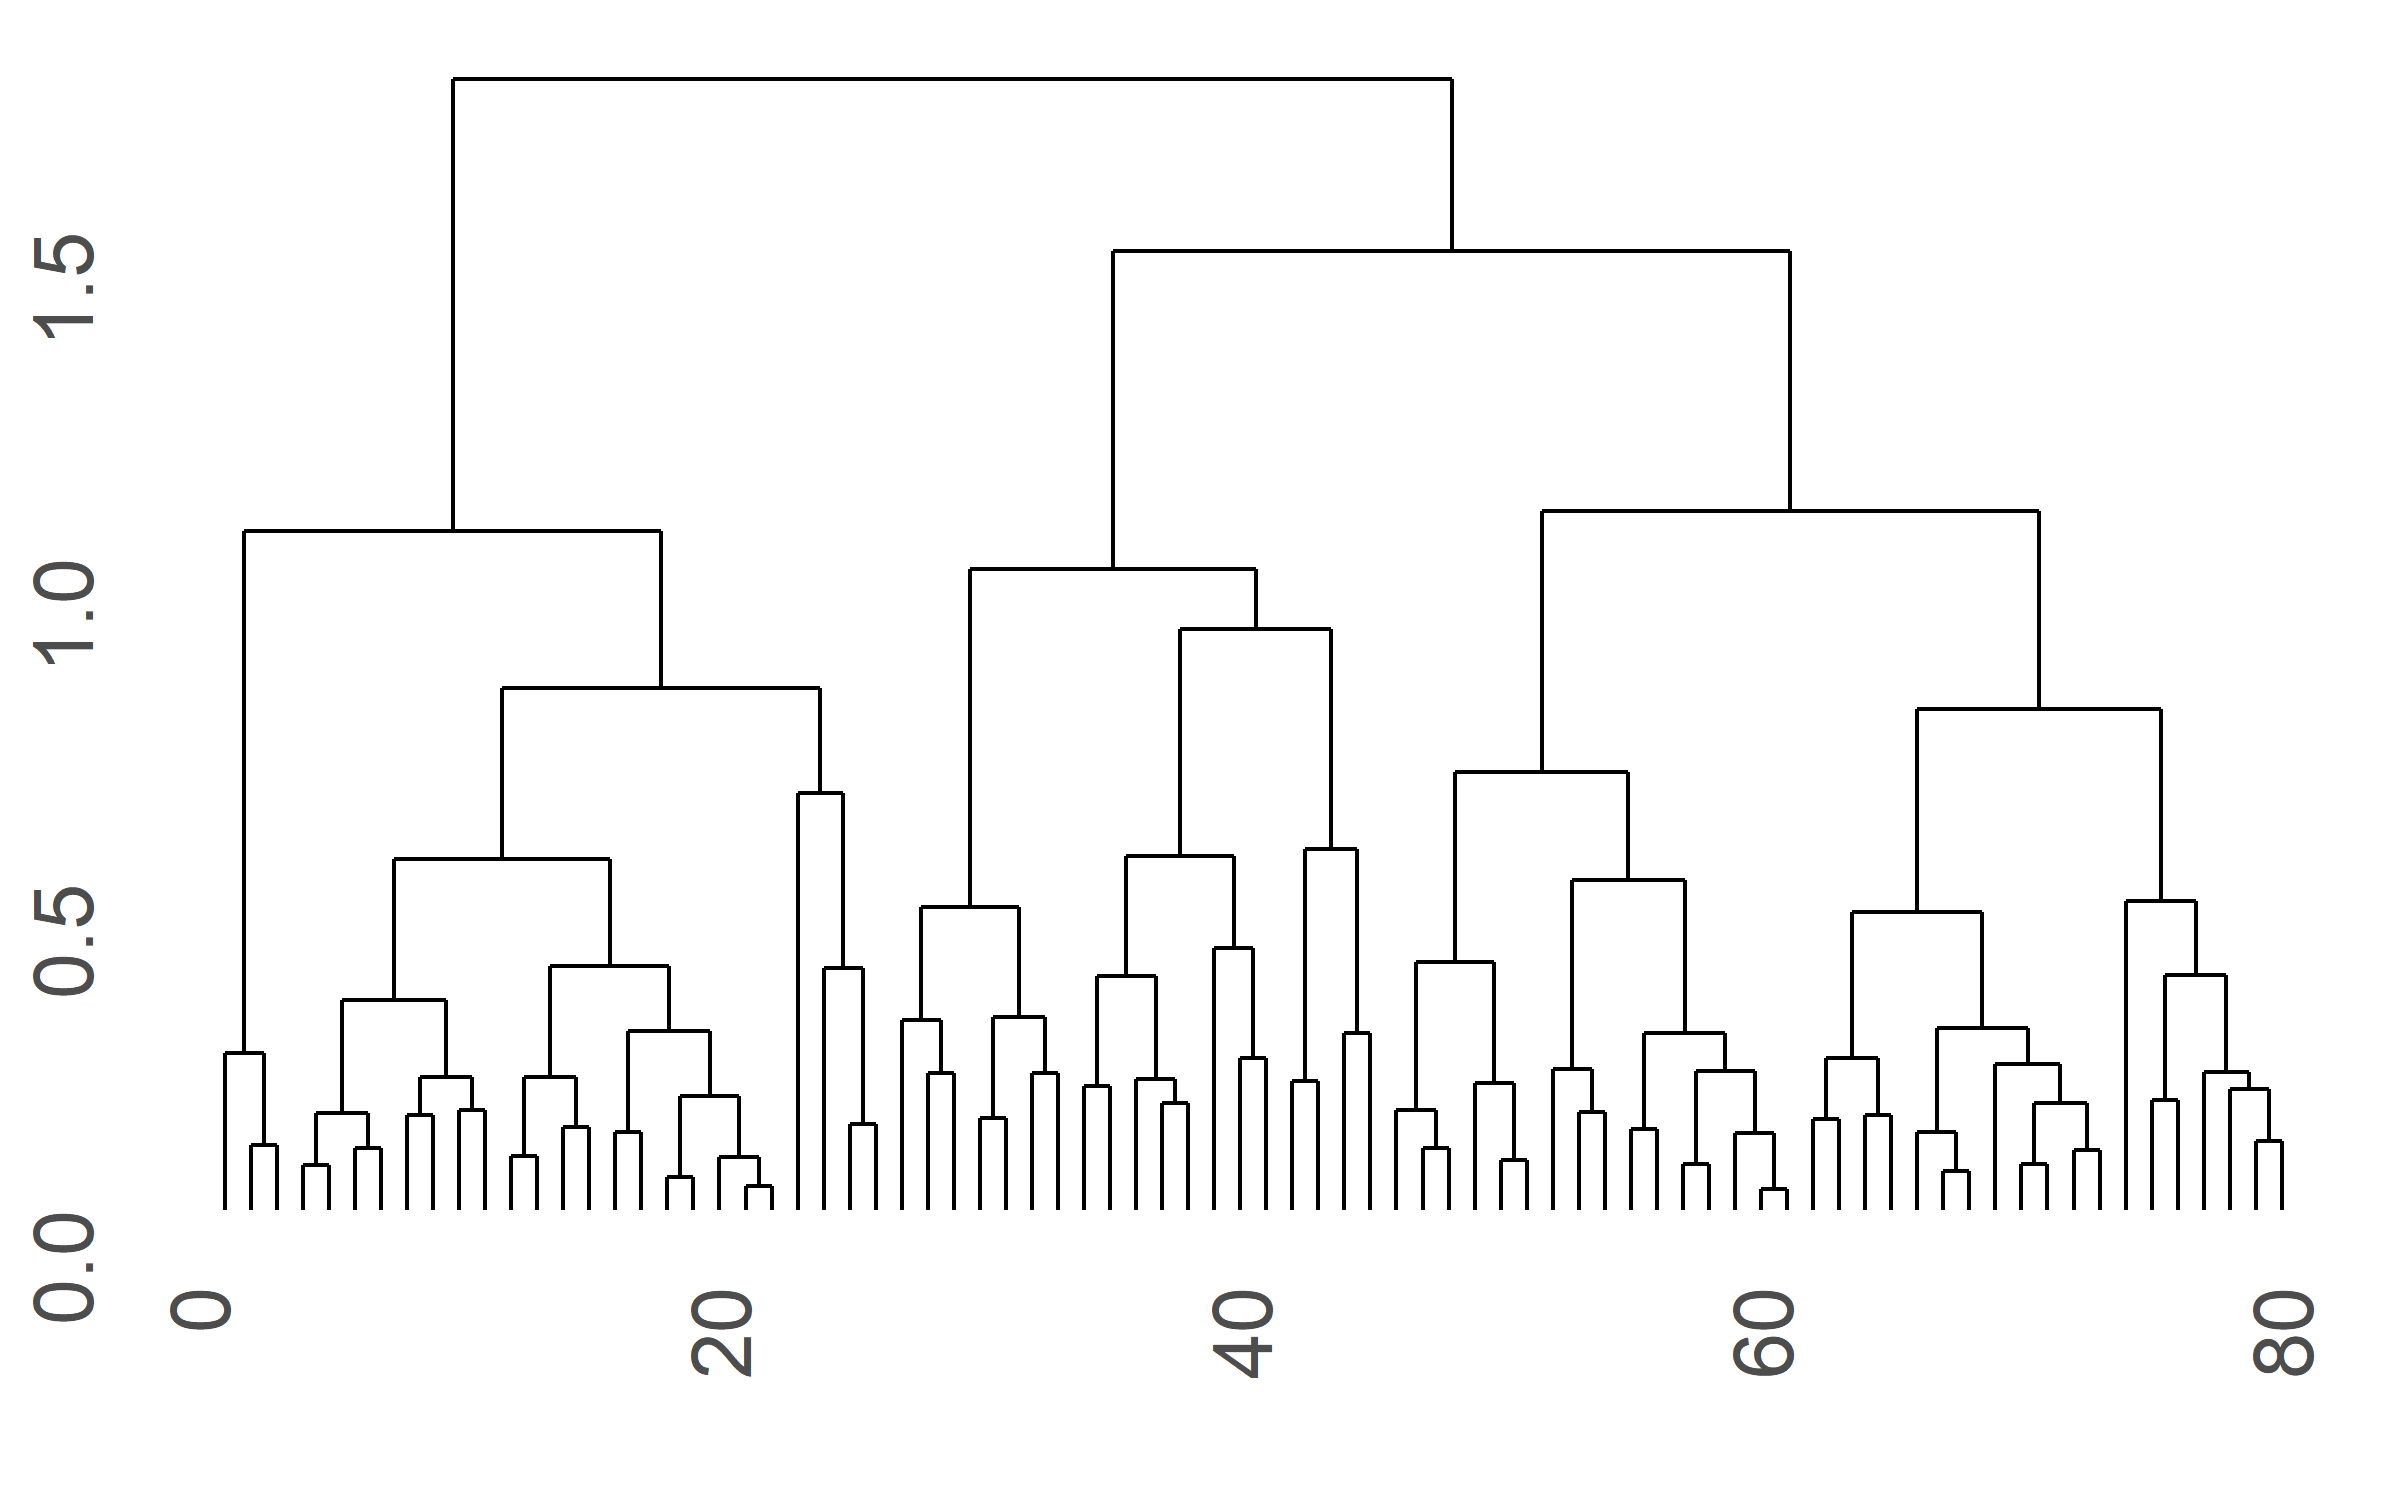
\includegraphics[width=0.8\textwidth]{img/dendrogram.png}
\caption{基频轮廓聚类树状图}
\label{den}
\end{figure}

将簇数设置为3时，得到聚类获得的基频轮廓如图\ref{f0}。

\begin{figure}[H]
\centering
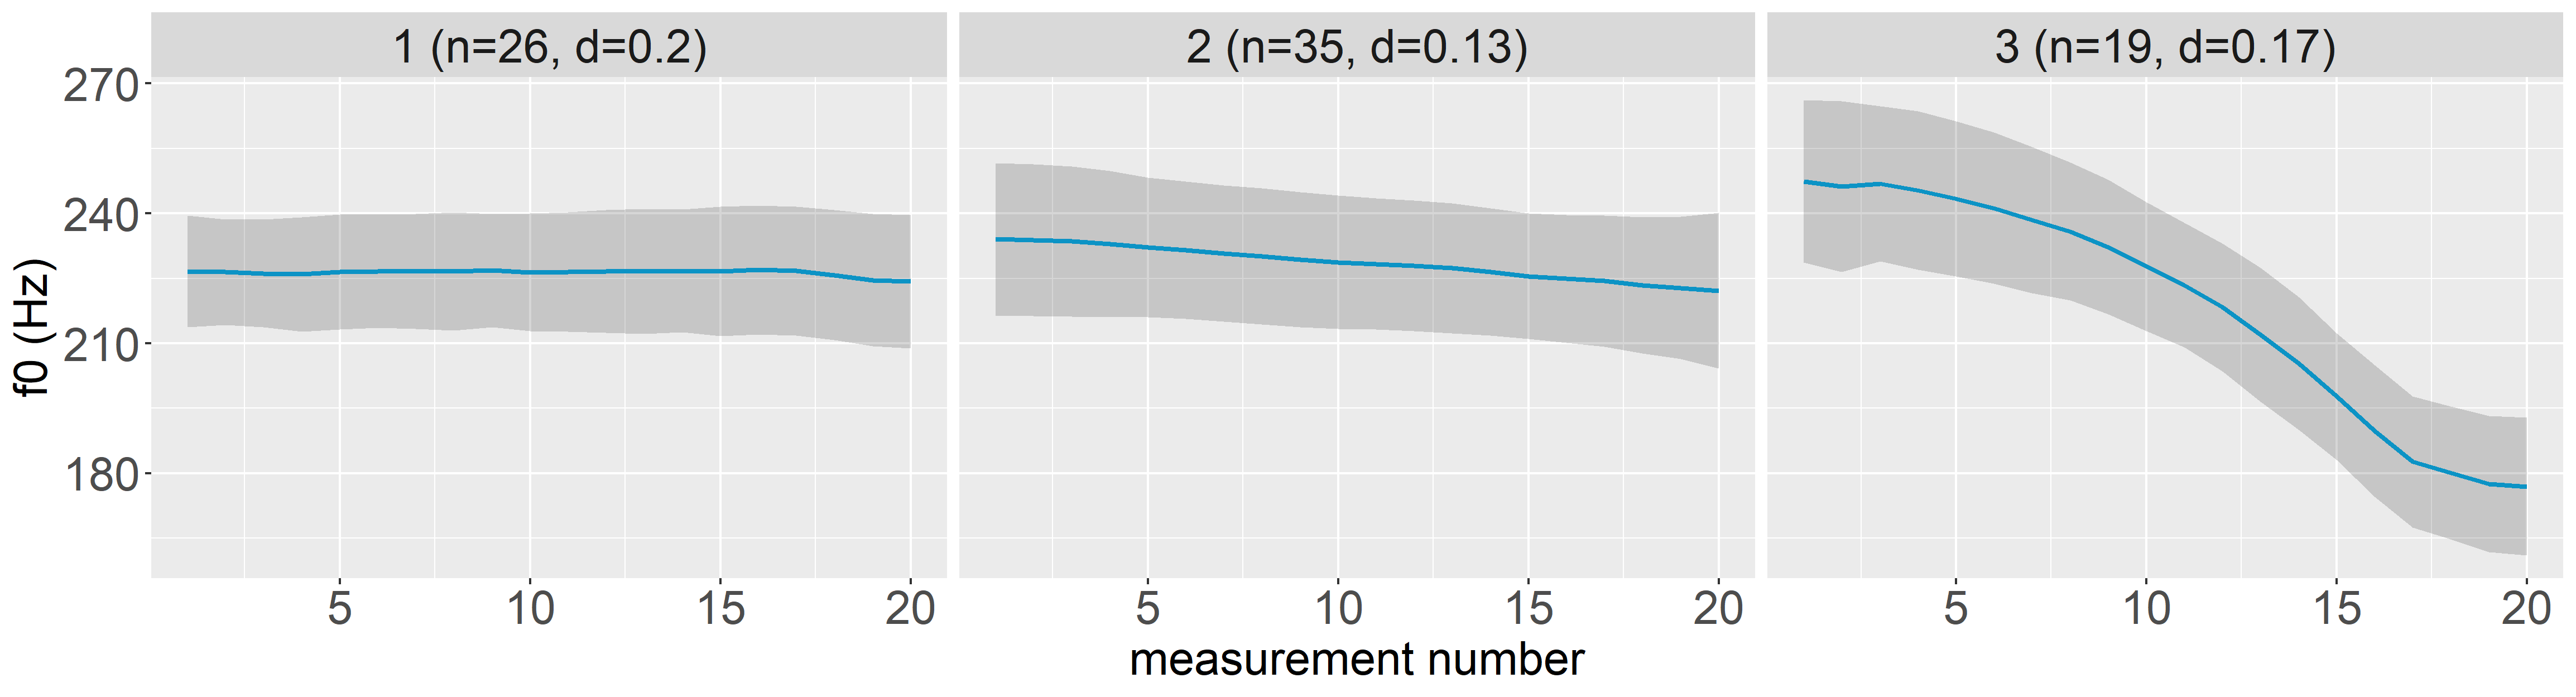
\includegraphics[width=0.8\textwidth]{img/plot_3.png}
\caption{基频轮廓}
\label{f0}
\end{figure}

其中簇1、2、3与人工标注的声调[H]、[HL]的对应如列联表\ref{toneclus}所示。

\begin{table}[H]
    \vspace{5pt}
    \centering
    \caption{声调-聚类簇列联表}
    \label{toneclus}
\begin{tabular}{c|ccc}
   \toprule
    \textit{} & 簇1 & 簇2 & 簇3 \\
    \midrule
  H & 25 & 25 & 0  \\
  HL & 1  & 10 & 19 \\
   \bottomrule
\end{tabular}
\end{table}

高调[H]样本主要集中于簇1和簇2，降调[HL]的样本集中在簇3，少部分分布在簇2。在“聚类结果与声调相互独立”的原假设下计算得到的期望频数与观测频数差异显著，$\chi ^{2}(2) = 45.42$，对应的显著性水平为$p = 1.37\times 10^{-10} \lll  0.001$。由此可见，聚类结果与声调之间存在高度相关性。

根据聚类结果和人工测量的基频，可以得出米亚罗话[H]调基频大约在210-240Hz之间，[HL]调基频大约从240-270Hz下降到150-180Hz。

以此为基准，可以测量出米亚罗话的表层声调在各个音节下有三种调型，如表\ref{to}所示。

\begin{table}[H]
    \vspace{5pt}
    \centering
    \caption{调型表}
    \label{to}
\begin{tabular}{c|cccc}
   \toprule
    & 单音节 & 双音节  & 三音节    & 四音节      \\
    \midrule
  (a) & H   & L.H  & L.H.H  & L.H.H.L  \\
(b) & HL  & L.HL & L.H.HL & L.H.H.HL \\
(c) & L   & H.L  & H.H.L  & L.H.H.L \\
   \bottomrule
\end{tabular}
\end{table}

其中，调型(c)仅仅应用在动词的屈折形态以及状貌词上。其他词汇均应用调型(a)和(b)。可以看出，米亚罗话每个词汇的表层声调似乎是可预测的，在下一节将具体讨论米亚罗话的底层声调和其如何推导到表层声调。

\section{底层声调}

正如\textcite{hsieh1999theoretical}和\textcite{lin2012no}所论证的，四土嘉绒语卓克基话的表层声调系统是可预测的。林幼菁指出卓克基话存在一个缺性声调（privative tone）系统，其底层是降调和零声调的对立，而在表层展现为词末音节降调和高低调的对立；且根据底层声调可以确定表层声调的表现。在米亚罗话中，底层同样存在词末音节降调和零声调的对立。本文采用V标示词末音节为零声调，V̂标示词末音节为降调。

米亚罗话的零声调和降调的对立具有词汇辨义作用，如表\ref{tonex}所示。

\begin{table}[H]
    \vspace{5pt}
    \centering
    \caption{双音节词汇声调最小对}
    \label{tonex}
\begin{tabular}{cc|cc}
   \toprule
    /$\varnothing$/ &  & /HL/ & \\
    {[L.H]} & & [L.HL] & \\
    \midrule
  {[kɐwu]} & “左面” &  [kɐ-wû] & “给” \\
   {[tə-mə]} & “女人” & [tə-mə̂] & “天空/雨” \\
   \bottomrule
\end{tabular}
\end{table}

米亚罗话零声调词应用调型(a)和(c)。生成零声调词需要应用的规则有：

\begin{enumerate}
    \setlength{\itemsep}{-0.3em}
    \item 音步分解（左）：从词的左端分解出双拍抑扬音步。
    \item 音步分解（右）：从词的右端分解出双拍扬抑音步。
    \item 弱化音步：余下的单音节均划为单拍音步。
    \item 强制高调：每个音步中心成分指派高调[H]。
    \item 插入高调：两个高调之间不带调值的音节指派高调[H]。
    \item 默认低调：剩余不带声调的音节指派低调[L]。
\end{enumerate}

相较于卓克基话的声调生成规则（\cite{lin2012no}），米亚罗话的的主要区别是弱化音步操作会对所有的单音节生效，而非卓克基话仅对非词首音节生效。

调型(a)的的规则使用顺序是：音步分解（左）、音步分解（右）、弱化音步、强制高调、插入高调、默认低调。如下例：

\begin{table}[H]
\begin{tabular}{ll}
           & kə-mə.rtsep “辣的” \\
词语         & kə.mə.rtsep      \\
1. 音步分解（左） & (kə.\textbf{mə})rtsep     \\
2. 音步分解（右） & N/A              \\
3. 弱化音步    & (kə.\textbf{mə})(\textbf{rtsep})   \\
4. 强制高调    & (kə.\ruby[g]{\textbf{mə}}{H})(\ruby[g]{\textbf{rtsep}}{H})   \\
5. 插入高调    & N/A              \\
6. 默认低调    & \ruby[g]{kə}{L}.\ruby[g]{mə}{H}.\ruby[g]{rtsep}{H}     \\
表面形式       & {[}L.H.H{]}     
\end{tabular}
\end{table}

调型(c)的规则使用顺序是：音步分解（右）、音步分解（左）、弱化音步、强制高调、插入高调、默认低调。如下例：

\begin{table}[H]
\begin{tabular}{lll}
           & ndze.ndzet “蹑手蹑脚” & te-wɐ.net “点灯（命令式）” \\
词语         & ndze.ndzet        & te.wɐ.net           \\
1. 音步分解（右） & (\textbf{ndze}.ndzet)        & te.(\textbf{wɐ}.net)           \\
2. 音步分解（左） & N/A               & N/A                 \\
3. 弱化音步    & N/A               & (\textbf{te})(\textbf{wɐ}.net)           \\
4. 强制高调    & (\ruby[g]{\textbf{ndze}}{H}.ndzet)        & (\ruby[g]{\textbf{te}}{H})(\ruby[g]{\textbf{wɐ}}{H}.net)           \\
5. 插入高调    & N/A               & N/A                 \\
6. 默认低调    & \ruby[g]{ndze}{H}.\ruby[g]{ndzet}{L}        & \ruby[g]{te}{H}.\ruby[g]{wɐ}{H}.\ruby[g]{net}{L}           \\
表面形式       & {[}H.L{]}         & {[}H.H.L{]}        
\end{tabular}
\end{table}

表面调型(b)只有词末音节会指派[HL]调，其余规则使用顺序与调型(a)相同。如下例：

\begin{table}[H]
\begin{tabular}{ll}
           & kʰa.jpɐ.lu.lu “蝴蝶” \\
词语         & kʰa.jpɐ.lu.lu      \\
1. 音步分解（左） & (kʰa.\textbf{jpɐ})lu.\ruby[g]{lu}{HL}      \\
2. 音步分解（右） & (kʰa.\textbf{jpɐ})(\textbf{lu}.\ruby[g]{lu}{HL})      \\
3. 弱化音步    & N/A                \\
4. 强制高调    & (kʰa.\ruby[g]{\textbf{jpɐ}}{H})(\ruby[g]{\textbf{lu}}{H}.\ruby[g]{lu}{HL})      \\
5. 插入高调    & N/A                \\
6. 默认低调    & \ruby[g]{kʰa}{L}.\ruby[g]{jpɐ}{H}.\ruby[g]{lu}{H}.\ruby[g]{lu}{HL}      \\
表面形式       & {[}L.H.H.HL{]}    
\end{tabular}
\end{table}
\chapter{与亲属语言的比较}

\section{词汇相似度的计算}

\textcite{lai2023lexical}整理了用于计算和历史比较的嘉绒语组语言同源词词表，其中包括291项概念。本文使用词表中的四土嘉绒语白湾话、马尔康话、脚木足话，以及茶堡嘉绒语的词汇材料进行词汇相似度的计算。\footnote{本小节使用的\textcite{lai2023lexical}数据库中的词汇，引用自\textcite{Jacques2016-bp}（茶堡嘉绒语）、\textcite{Zhang2020-ya}（四土嘉绒语白湾话）、\textcite{prins2011web}（四土嘉绒语脚木足话）、\textcite{Huang1992}（四土嘉绒语马尔康话）。本章其他小节也使用了\textcite{Nagano2013-hy}（四土嘉绒语梭磨话）、\textcite{Lin-2016-dr}（四土嘉绒语卓克基话）、\textcite{Gong2018-aw}（日部嘉绒语）的词汇数据。}

对于词表中的概念，有271项可以对应到米亚罗话的词汇。本文对相似度的定义为：若两个形式分别为$x$和$y$，莱文斯坦距离为$d(x,y)$，相似度S(x,y)为

\[
S(x,y)=1-\frac{d(x,y)}{\max(|x|,|y|)}
\]

表\ref{simtomyaglo}列出了各语言点与米亚罗话的平均相似度。可以看到，在三个四土嘉绒语方言中，米亚罗话与马尔康话的词汇相似度最高（0.512），其次是脚木足话（0.435），与白湾话的表层相似度最低（0.338）；而作为外群的茶堡嘉绒语相似度明显更低（0.231）。

\begin{table}[H]
\vspace{5pt}
    \centering
    \caption{各语言点与米亚罗话的词汇相似度}
    \label{simtomyaglo}
\begin{tabular}{lccc}
\toprule
语言点 & 所属 & 计算词数 & 平均相似度 \\
\midrule
马尔康话 & 四土嘉绒语 & 228 & 0.512 \\
脚木足话 & 四土嘉绒语 & 220 & 0.435 \\
白湾话   & 四土嘉绒语 & 268 & 0.338 \\
茶堡嘉绒语   & 东部嘉绒语组 & 270 & 0.231 \\
\bottomrule
\end{tabular}
\end{table}

四个四土嘉绒语方言两两之间的相似度矩阵如表\ref{simmatrix}所示。这一格局与\textcite{gates2014situ}基于互通度和方言学调查得出的结论大体吻合：米亚罗话处在四土嘉绒语中东部方言区与南部方言区的交界处，在词汇上靠近以马尔康话为代表的中部方言。

\begin{table}[H]
\vspace{5pt}
    \centering
    \caption{四土嘉绒语方言的词汇相似度矩阵}
    \label{simmatrix}
\begin{tabular}{lcccc}
\toprule
       & 米亚罗话 & 白湾话 & 马尔康话 & 脚木足话 \\
\midrule
米亚罗话 & ---   & 0.338 & 0.512 & 0.435 \\
白湾话   & 0.338 & ---   & 0.434 & 0.445 \\
马尔康话 & 0.512 & 0.434 & ---   & 0.494 \\
脚木足话 & 0.435 & 0.445 & 0.494 & ---   \\
\bottomrule
\end{tabular}
\end{table}

\section{重要音系特征的比较}

\subsection{声母}

正如第\ref{charonset}章所描写的，米亚罗话的声母保留了丰富的复辅音。这一特征在四土嘉绒语各方言中是共有的。表\ref{clusterretention}列举了若干带复辅音声母的词汇，可以看到/mŋ-/、/mbr-/、/spj-/、/zd-/、/skr-/、/mkr-/等辅音簇在四个方言中整齐对应、几乎原样保留，茶堡嘉绒语也大体一致。

\begin{table}[H]
\vspace{5pt}
    \centering
    \caption{四土嘉绒语方言中的复辅音声母}
    \label{clusterretention}
\begin{tabular}{lllllll}
\toprule
释义 & 米亚罗话 & 白湾话 & 马尔康话 & 脚木足话 & 茶堡嘉绒语 \\
\midrule
五 & kə-mŋu      & kəmŋɐj    & kə mŋo    & kəmŋi      & kɯmŋu \\
高 & kə-mbro     & mbro      & kə mbro   & kəmbro     & mbro \\
长 & kə-skrin    & skrēn     & kə skrᴇn  & kəskriʔn   & zri \\
狼 & spjaŋkə     & spjaŋkə   & spjɑŋ kə  & spjankə    & spjaŋkɯ \\
云 & zdem        & zdiəm     & zdᴇm      & zdeʔm      & zdɯm \\
横 & kə-ŋa-mkrak & o-mkrāk   & kɑ mkrɑk  & kəŋamkrak  & ndom \\
\bottomrule
\end{tabular}
\end{table}

\textcite{Gong2018-aw}将四土嘉绒语分为“去鼻冠音”（deprenasalization）类型和“弱化”（leniting）类型。对于古单辅音清爆发音声母，去鼻冠音方言会保留清爆发音，而弱化方言会发生浊化；对于古鼻冠音声母，去鼻冠音方言会去鼻化甚至擦音化，而弱化方言则会保留鼻冠音。表\ref{deprelen}比较了典型的弱化方言白湾话、典型的去鼻冠方言卓克基话和米亚罗话的一些词汇。可以看出，米亚罗话更接近去鼻冠方言。

\begin{table}[H]
\vspace{5pt}
    \centering
    \caption{四土嘉绒语去鼻冠音和弱化方言的比较}
    \label{deprelen}
\begin{tabular}{l|lll}
\toprule
          & 米亚罗话     & 卓克基话   & 白湾话       \\
\midrule
给   & ka-wu    & ka-wə  & ka-ⁿbi    \\
变老 & kə-waj   & kə-wi  & ka-ⁿbɐj   \\
聋子      & tɐ-wo    & ta-wo  & ta-ⁿbo    \\
衣服     & tə-wâ   & tə-wa  & tə-ⁿga    \\
蛋       & ta-gam   & ta-gam & ta-ⁿgəm   \\
吃    & ka-ze    & ka-za  & ka-ⁿdziɛ̂ \\
脸      & ta-jû   & ta-jo  & ta-ɟɐ̂    \\
羊     & kəjo     & kə.jo  & kə.ɟók    \\
儿子       & tə-tse   & tə-tsa & tə-ziɛ̂   \\
10       & ʃtɕi     & ɕtɕiɛ  & zɟé       \\
面粉     & ta-pet   & ta-pat & ta-viɛ́t  \\
雪      & ta-jpêt & ta-jpa & ta-jviɛ̂  \\
做    & ka-pe    & ka-pa  & ka-viɛ̂   \\
头      & ta-ku    & ta-ko  & ta-wo    \\
\bottomrule
\end{tabular}
\end{table}

\subsection{韵母}

米亚罗话韵尾位置可以出现/-p, -t, -k, -s/等辅音；从同源词看，米亚罗常保留口腔闭塞韵尾，而脚木足话常在韵尾前出现喉塞成分，茶堡和日部嘉绒语中则常见/-ʁ, -β, -v, -ʔ/等擦音、喉塞音韵尾。表\ref{tab:coda-comparison}列出了部分词汇。

\begin{table}[H]
	\centering
	\caption{亲属语言的韵尾辅音}
	\label{tab:coda-comparison}
	\vspace{5pt}
	\begin{tabular}{llllll}
		\toprule
		释义 & 米亚罗话 & 白湾话 & 脚木足话 & 茶堡嘉绒语 & 日部嘉绒语\\
		\midrule
		眼睛 & tə-mɲɐk & tə-mɲāk & təmɲaʔk & tɯ-mɲaʁ & ɐ-mɲɐ̂ʁ\\
		手 & tɐ-jɐ̂k & ta-jāk & tajiʔk & tɯ-jaʁ & tə-jɐ̂ʁ\\
		猪 & pɐk & piāk & pak &  paʁ & pɐ̂ʁ\\
		妻子 & tɐ-rʒep1 & ta-rɟēp & tarɟaʔp & tɤ-rʑaβ & və-rɟev\\
		山羊 & tsʰut1 & tɕhə̂ & tʃhət & tshɤt & tsɯtɑ\\
		七 & kə-ʃnəs2 & kəɕnɐ̄s & kəʃnəʔs & kɯɕnɯz & kɯsnɑz\\
		\bottomrule
	\end{tabular}
\end{table}

茶堡嘉绒语[tɯ-mɲaʁ]“眼睛”、[tɯ-jaʁ]“手”、[paʁ]“猪”和日部嘉绒语[ɐ-mɲɐ̂ʁ]、[tə-jɐ̂ʁ]、[pɐ̂ʁ]都用小舌擦音对应米亚罗、白湾和脚木足的[-k]。而“妻子”一词，茶堡嘉绒语[tɤ-rʑaβ]和日部嘉绒语[və-rɟev]则用双唇和唇齿擦音对应米亚罗话的[-p]。这可能说明茶堡和日部嘉绒语的韵尾爆发音有弱化倾向。

对于韵尾的复辅音，四土嘉绒语中除了米亚罗话之外，目前仅在白湾话和梭磨话中发现了词末复辅音。其中白湾话的词末复辅音仅限于动词发生论元标记的形态学过程时可以产生\cite{zhang2016phonologie}，词干的韵尾位置不允许出现复辅音。而梭磨话和米亚罗话一样允许在词干位置出现复辅音。表\ref{clustercoda}列出了米亚罗话中的词干复辅音词汇在白湾话、卓克基话、梭磨话、茶堡嘉绒语中的对应词。

\begin{table}[H]
\vspace{5pt}
    \centering
    \caption{四土嘉绒语方言中的复辅音韵尾}
    \label{clustercoda}
\begin{tabular}{lllllll}
\toprule
释义 & 米亚罗话 & 白湾话 & 卓克基话 & 梭磨话 & 茶堡嘉绒语 \\
\midrule
影子 & ta-jips      & tajəs    & tajəp̚    & tajəps      & taʁjɯβ \\
手镯 & zgrôks     & ---      & zgruk   & sgroks     & zgroʁ \\
灰尘 & ta-jleps    & ---     & tilap̚  & tajpops   & --- \\
暗的 & kə-rniks     & kərȵis   & kərȵəp̚  & kərȵəps  & 	qanɯ \\
\bottomrule
\end{tabular}
\end{table}

\section{小结}

综合本文前面各章的描写与本章的比较，米亚罗话作为四土嘉绒语东南端的一个方言，其音系既体现了嘉绒语组共有的形态—音系复杂性，又呈现出区别于其他方言的特征。本节就米亚罗话的音系类型作如下总结。

第一，从保守性来看，米亚罗话较为完整地保留了复辅音系统与韵尾辅音系统。声母方面，米亚罗话允许最多三个辅音组成的复辅音簇，可析出冠音、首音、介音三个位置；调查所得的146种复辅音类型与白湾话、马尔康话、脚木足话乃至茶堡嘉绒语对应较为整齐，表明嘉绒语组特征性的复辅音系统在米亚罗话中得到较为完整保留。韵尾方面，米亚罗话保留了/-p, -t, -k/等爆发音韵尾，与茶堡嘉绒语和日部嘉绒语的韵尾擦音化倾向（/-ʁ, -β, -v/）形成对照。此外，米亚罗话允许/-ms, -ks, -ps, -ŋs/四种复辅音韵尾出现于词干位置，这一特征在四土嘉绒语方言中较为少见，可能展现与白湾话、卓克基话等方言不同的保守性。

第二，从创新性来看，米亚罗话属于\textcite{Gong2018-aw}所论的去鼻冠音方言：古单辅音清爆发音声母在米亚罗话中保留清爆发音而未浊化，古鼻冠音声母则去鼻化甚至擦音化。这一表现与卓克基话一致，而明显不同于以白湾话为代表的弱化方言。

第三，从声调系统来看，米亚罗话与卓克基话、小金话一样，有着底层零声调与词末降调对立的缺性声调系统。实验语音学分析显示，其声调对立的核心声学相关物集中于词末音节的末端基频与基频斜率，而非起点高度或时长。

%---------------------------------------------------------------------
%	参考文献
%---------------------------------------------------------------------

% 生成参考文献页
\printbibliography

%---------------------------------------------------------------------
%	附录部分
%---------------------------------------------------------------------

% 附录部分使用单独的字母序号
\appendix
\providecommand{\ipa}[1]{#1}
\providecommand{\audioGlossIndex}[1]{}
\providecommand{\audioGlossGroup}[1]{%
  \par\medskip\noindent{\large\bfseries #1}\par\nopagebreak\vspace{0.15em}%
}
\providecommand{\audioGlossEntry}[2]{%
  \audioGlossIndex{#1}%
  \noindent\hangindent=2.6em\hangafter=1\textbf{\ipa{#1}}\quad #2\par%
}
\chapter{四土嘉绒语米亚罗话词表}
\noindent 本词表根据共收词 1366 条。词条以国际音标为索引项排序。为方便数据处理，以词末“1”标记零声调、“2”标记降调。
\begingroup
\small
\setlength{\columnsep}{1.35em}
\setlength{\parindent}{0pt}
\setlength{\parskip}{0.08em}
\begin{multicols}{2}
\raggedcolumns
\audioGlossGroup{\ipa{ɐ}}
\audioGlossEntry{ɐkɤ2}{叔叔（无亲戚关系）/岳父}
\audioGlossEntry{ɐnə2}{阿姨（无亲戚关系）/岳母}
\audioGlossEntry{ɐrɐk1}{酒}
\audioGlossEntry{ɐrji.lu2}{去年}
\audioGlossEntry{ɐrji2}{从前}
\audioGlossEntry{ɐrji2}{砾石}
\audioGlossEntry{ɐʃlu1}{昨天}
\audioGlossEntry{ɐʃnətʃɿ1}{前天}
\audioGlossEntry{ɐwurərə1}{蜗牛}

\audioGlossGroup{\ipa{b}}
\audioGlossEntry{bɐlə2}{没有角的牦牛}
\audioGlossEntry{bejwɐ2}{工钱/请和尚念经的费用}
\audioGlossEntry{bəlerler1}{滚}
\audioGlossEntry{bjoŋpu2}{疯子}
\audioGlossEntry{bjoŋpu2}{神经病}
\audioGlossEntry{boŋti1}{裹腿}
\audioGlossEntry{boset1 kɐ-lɐt2}{磨刀}
\audioGlossEntry{brɐli2 kɐpe1}{地震/打雷}
\audioGlossEntry{brɐri2}{地震}
\audioGlossEntry{buktʃʰaj2}{䥽}
\audioGlossEntry{busmuk1}{发霉}

\audioGlossGroup{\ipa{d}}
\audioGlossEntry{dʒoŋpesprɐk1}{小腰带}
\audioGlossEntry{dʑu1}{竹子}

\audioGlossGroup{\ipa{ə}}
\audioGlossEntry{əjesmɐkji1}{嫉妒}
\audioGlossEntry{əjo1}{别人}
\audioGlossEntry{əʃkʰaj2}{刚才}
\audioGlossEntry{əʃnə2}{今天}

\audioGlossGroup{\ipa{g}}
\audioGlossEntry{ganpə2}{箱子}
\audioGlossEntry{gəmbɐ2}{庙}
\audioGlossEntry{gən1}{很}
\audioGlossEntry{gorwu2}{青冈树/橡树}

\audioGlossGroup{\ipa{j}}
\audioGlossEntry{jɐ-ŋa.jpʰit1}{走散}
\audioGlossEntry{ja-ntʃʰan1}{（詈语）滚}
\audioGlossEntry{jɐ-rʒəwlok1}{（詈语）滚}
\audioGlossEntry{jɐ-stokej1}{（詈语）滚}
\audioGlossEntry{jɐkpɐʒe1}{扇巴掌}
\audioGlossEntry{jɐmtse1}{炒菜锅}
\audioGlossEntry{jɑŋ1 mɐ1}{自行车}
\audioGlossEntry{jɑŋ1 tɕan2}{肥皂}
\audioGlossEntry{jɑŋ1 xu1}{火柴}
\audioGlossEntry{jɑŋ1 y2}{土豆}
\audioGlossEntry{jɐtsɿ1}{鸭子}
\audioGlossEntry{jimɐpɐt2}{玉米面粉}
\audioGlossEntry{jimotsej1}{儿媳}
\audioGlossEntry{jin1 tʃən1 kɐ-lɐt2}{扎针}
\audioGlossEntry{jipʰɐje1}{女婿}
\audioGlossEntry{jixa1}{全都}
\audioGlossEntry{jkɐr2}{铜/绿松石}
\audioGlossEntry{jo1/əɲi2}{我们}
\audioGlossEntry{joŋdʒom2}{万字}

\audioGlossGroup{\ipa{k}}
\audioGlossEntry{kɐ-gu2}{钻}
\audioGlossEntry{kɐ-jdɐ2}{解开}
\audioGlossEntry{kɐ-je1}{回}
\audioGlossEntry{kɐ-ji2}{种/向下移动/下山}
\audioGlossEntry{kɐ-jməs1}{忘记}
\audioGlossEntry{kɐ-jni2}{揉面}
\audioGlossEntry{kɐ-jok1}{仰头/抬/悬挂}
\audioGlossEntry{kɐ-jru2}{寻找（近）}
\audioGlossEntry{kɐ-jwa2}{锄地/挖地}
\audioGlossEntry{kɐ-kɤ2}{买}
\audioGlossEntry{kɐ-kʰɐ2}{恨}
\audioGlossEntry{kɐ-kʰɐs1}{生气}
\audioGlossEntry{kɐ-kʰo1}{晒/烤}
\audioGlossEntry{kɐ-kor1}{帮助}
\audioGlossEntry{kɐ-kro1}{分}
\audioGlossEntry{kɐ-ksər2}{炒菜}
\audioGlossEntry{kɐ-kʃət1}{出去/升起/出现}
\audioGlossEntry{kɐ-ktor2}{撒}
\audioGlossEntry{kɐ-lan2}{答}
\audioGlossEntry{kɐ-lɐt2}{下雨/生蛋/开花/写/发/打}
\audioGlossEntry{kɐ-lok1}{放}
\audioGlossEntry{kɐ-lu1}{瞎子/独眼龙}
\audioGlossEntry{kɐ-mɐli2}{欠}
\audioGlossEntry{kɐ-mɐrpɐk1}{扛}
\audioGlossEntry{kɐ-mbri2}{玩耍}
\audioGlossEntry{kɐ-mdə2}{到}
\audioGlossEntry{kɐ-mnik1}{吞/咽}
\audioGlossEntry{kɐ-mɲo2}{准备}
\audioGlossEntry{kɐ-mpʰɐr1}{卖}
\audioGlossEntry{kɐ-mpʰər2}{包/花苞/包围/披衣服}
\audioGlossEntry{kɐ-mto1}{看见}
\audioGlossEntry{kɐ-mtsɐk1}{跳}
\audioGlossEntry{kɐ-mtsɿ1}{钉/钉子}
\audioGlossEntry{kɐ-mtsi2}{安家}
\audioGlossEntry{kɐ-mtɕi2}{要}
\audioGlossEntry{kɐ-mut1}{灌/喝}
\audioGlossEntry{kɐ-nɐ-sŋu1}{骂}
\audioGlossEntry{kɐ-nɐ.kʰu1}{喊}
\audioGlossEntry{kɐ-nɐ.lɐ2}{愿意}
\audioGlossEntry{kɐ-nɐ.mi2}{骑}
\audioGlossEntry{kɐ-nɑ.ŋsəŋsət1}{闻}
\audioGlossEntry{kɐ-na.ntsu1}{看}
\audioGlossEntry{kɐ-nɐ.ntɕi2}{摔}
\audioGlossEntry{kɐ-nɐ.wze.wzet1}{犹豫}
\audioGlossEntry{kɐ-nɐjo1}{等候}
\audioGlossEntry{kɐ-nɐkʰij2}{欺负}
\audioGlossEntry{kɐ-nɐkti2}{尊敬}
\audioGlossEntry{kɐ-nɐmətsət1}{讨论}
\audioGlossEntry{kɐ-nandi1}{相信}
\audioGlossEntry{kɐ-nɐŋe1}{喜欢/爱好}
\audioGlossEntry{kɐ-nɑŋi2}{晒太阳}
\audioGlossEntry{kɐ-nantsɿ1}{保守秘密}
\audioGlossEntry{kɐ-nɐntwɐr1}{甩}
\audioGlossEntry{kɐ-nantɕi2}{跺脚}
\audioGlossEntry{kɐ-nɐri2}{笑}
\audioGlossEntry{kɐ-nɐtselet1}{摸}
\audioGlossEntry{kɐ-nɐtʃɐp2}{隔着}
\audioGlossEntry{ka-ndu1}{得到}
\audioGlossEntry{kɐ-ndun2}{读}
\audioGlossEntry{kɐ-ndʒɿk1}{追赶}
\audioGlossEntry{kɐ-nə-ntsʰok1}{舔}
\audioGlossEntry{kɐ-nə.mɲɐk1}{射/看上某人}
\audioGlossEntry{kɐ-nə.ne1}{休息}
\audioGlossEntry{kɐ-nə.ŋkʰɐk1}{啃}
\audioGlossEntry{kɐ-nə.pjɐms2}{烤火}
\audioGlossEntry{kɐ-nə.rtsɿ2}{爬}
\audioGlossEntry{kɐ-nə.ʒdɐr1}{害怕}
\audioGlossEntry{kɐ-nə.ʒgre1}{抵住}
\audioGlossEntry{kɐ-nə2}{坐/住/在}
\audioGlossEntry{kɐ-nəgo2}{生病}
\audioGlossEntry{kɐ-nəjɐ1}{抢劫}
\audioGlossEntry{kɐ-nəkʰəstə1}{退}
\audioGlossEntry{kɐ-nəŋkros2}{分手}
\audioGlossEntry{kɐ-nənok1}{蘸}
\audioGlossEntry{kɐ-nəptekpe1}{崇拜}
\audioGlossEntry{kɐ-nəsɑŋɐrtɕis1}{升天}
\audioGlossEntry{kɐ-nəʃneti1}{可靠}
\audioGlossEntry{kɐ-nəʃpəs2}{模仿}
\audioGlossEntry{kɐ-nəskorwe1}{绕过去}
\audioGlossEntry{kɐ-nəterse1}{升天}
\audioGlossEntry{kɐ-nətɕok1}{赊账}
\audioGlossEntry{kɐ-nəwlu1}{骗}
\audioGlossEntry{kɐ-nəwʃɿ1}{认得}
\audioGlossEntry{kɐ-nəʒgrɐ2}{跨}
\audioGlossEntry{kɐ-ŋɐlɐlɐt2}{打架}
\audioGlossEntry{kɐ-ŋɐrdu1}{遇见}
\audioGlossEntry{kɑ-ŋgu1}{喂}
\audioGlossEntry{ka-ntɐr2}{发抖}
\audioGlossEntry{ka-ntat1}{蛰}
\audioGlossEntry{ka-ntʰe.ntʰen2}{伸懒腰}
\audioGlossEntry{ka-ntʃʰe1}{杀/宰}
\audioGlossEntry{kɐ-ntʃɿ2}{搬}
\audioGlossEntry{kɐ-ntʃit1}{含/握}
\audioGlossEntry{kɐ-ntɕʰi2}{挑选}
\audioGlossEntry{kɐ-nus2}{敢}
\audioGlossEntry{kɐ-pɐs2}{吃粉状食物}
\audioGlossEntry{kɐ-pe1}{做/唱}
\audioGlossEntry{kɐ-pʰɐk2}{砍柴/拆开}
\audioGlossEntry{kɐ-pʰit2}{扔/掷/吐/丢}
\audioGlossEntry{kɐ-pʰo2}{躲}
\audioGlossEntry{kɐ-pʰo2}{逃跑}
\audioGlossEntry{kɐ-pʰok2}{舀}
\audioGlossEntry{kɐ-pʰot1}{折/摘/取下}
\audioGlossEntry{kɐ-pʰroŋ2}{呛}
\audioGlossEntry{kɐ-pʰuk1}{撑开}
\audioGlossEntry{kɐ-pik1}{过滤}
\audioGlossEntry{kɐ-pje1}{捉/拿/钓鱼}
\audioGlossEntry{kɐ-pkur2}{背/怀孕}
\audioGlossEntry{kɐ-po1}{纺}
\audioGlossEntry{kɐ-prɐk1}{牵/栓}
\audioGlossEntry{kɐ-pri1}{撕}
\audioGlossEntry{kɐ-pʃɐm2}{晒谷子/散开/撒落}
\audioGlossEntry{kɐ-ptsəm2}{闭/抿嘴}
\audioGlossEntry{kɐ-ptʃɿ2}{熬油/煎/融化}
\audioGlossEntry{kɐ-ptʃo2}{用}
\audioGlossEntry{kɐ-pu2}{来}
\audioGlossEntry{kɐ-pu2}{烤}
\audioGlossEntry{kɐ-rɐ-ntsək1}{切}
\audioGlossEntry{kɐ-rɐ-wʃɿ1}{撕开}
\audioGlossEntry{kɐ-rɐ.mɐ2}{劳动}
\audioGlossEntry{kɐ-rɐ.tsʰɐt1}{量}
\audioGlossEntry{kɐ-rɐkʃok1}{搔痒}
\audioGlossEntry{kɐ-rɐkzet2}{抚养}
\audioGlossEntry{kɐ-rɐli2}{赔偿}
\audioGlossEntry{kɐ-rɐpə1}{繁衍}
\audioGlossEntry{kɐ-rɐpʰu1}{预估}
\audioGlossEntry{kɐ-rɐpo1}{摞}
\audioGlossEntry{kɐ-rɐtʃɐk1}{踩}
\audioGlossEntry{kɐ-rɐɕi2}{拉}
\audioGlossEntry{kɐ-rɐɕiɕi2}{搓}
\audioGlossEntry{kɐ-rə1}{扫}
\audioGlossEntry{kɐ-rəŋne1}{听}
\audioGlossEntry{kɐ-rəsɿso2}{思考}
\audioGlossEntry{kɐ-rəsɿsu2}{活下来}
\audioGlossEntry{kɐ-rjep1}{站}
\audioGlossEntry{kɐ-rkok1}{抱}
\audioGlossEntry{kɐ-rku1}{装}
\audioGlossEntry{kɐ-rme1}{睡}
\audioGlossEntry{kɐ-rŋe1}{借入/借出（物品）}
\audioGlossEntry{kɐ-rŋɤ2}{蹲}
\audioGlossEntry{kɐ-rŋu2}{炒}
\audioGlossEntry{kɐ-rtut1}{缠}
\audioGlossEntry{kɐ-rtɕik1}{跑/快快/逃走}
\audioGlossEntry{kɐ-ru2}{寻找（远）}
\audioGlossEntry{kɐ-rwɐs2}{起床/起来}
\audioGlossEntry{kɐ-rzək1}{剪/绞掉}
\audioGlossEntry{kɐ-sa.jpʰit1}{遗失vt}
\audioGlossEntry{kɐ-sɐ.mnə1}{堆}
\audioGlossEntry{kɐ-sɐ.pʰur2}{掸灰}
\audioGlossEntry{kɐ-sɐ.tʰərə2}{连接}
\audioGlossEntry{kɐ-sɐ.tselet1}{摇头}
\audioGlossEntry{kɐ-sɐ.tsəntsok1}{粘}
\audioGlossEntry{kɐ-sɐ.ɕet1}{梳}
\audioGlossEntry{kɐ-sɐje1}{开始}
\audioGlossEntry{kɐ-sɐr2}{娶}
\audioGlossEntry{kɐ-sɐsət1}{连根拔起}
\audioGlossEntry{kɐ-sɐstu2}{弄正}
\audioGlossEntry{kɐ-sɐtselet1}{移动}
\audioGlossEntry{kɐ-sɐtʃi.tʃi2}{顺便}
\audioGlossEntry{kɐ-sɐtɕilu2}{混合/和面/搅拌}
\audioGlossEntry{kɐ-sɐwjan2}{公平}
\audioGlossEntry{kɐ-sɐwustə2}{收集}
\audioGlossEntry{kɐ-səkʃut1}{教}
\audioGlossEntry{kɐ-set1}{杀死}
\audioGlossEntry{kɐ-ʃɐko1}{搀扶}
\audioGlossEntry{kɐ-ʃɐtʃəndu1}{换}
\audioGlossEntry{kɐ-ʃejnə1}{责怪}
\audioGlossEntry{kɐ-ʃəm1}{收}
\audioGlossEntry{kɐ-ʃəptɐk1}{记得}
\audioGlossEntry{kɐ-ʃərŋət1}{低头}
\audioGlossEntry{kɐ-ʃɿ2}{懂}
\audioGlossEntry{kɐ-ʃɿʒdɐr2}{威胁}
\audioGlossEntry{kɐ-ʃkət1}{吃完}
\audioGlossEntry{kɐ-ʃkre1}{筛}
\audioGlossEntry{kɐ-ʃmo1}{偷}
\audioGlossEntry{kɐ-ʃpe1}{会}
\audioGlossEntry{kɐ-ʃti1}{塞/捂嘴}
\audioGlossEntry{kɐ-ʃtɕi1}{传染}
\audioGlossEntry{kɐ-sɿ-mdɐm2}{使凝固}
\audioGlossEntry{kɐ-sɿ2}{靠}
\audioGlossEntry{kɐ-sɿkɤ1}{土葬/埋}
\audioGlossEntry{kɐ-sɿlɐp1}{学/练习}
\audioGlossEntry{kɐ-sɿmtso2}{告诉}
\audioGlossEntry{kɐ-sɿpʰis2}{擦}
\audioGlossEntry{kɐ-sɿru2}{睁开}
\audioGlossEntry{kɐ-sɿstɕi2}{借出（钱）}
\audioGlossEntry{kɐ-sɿwule1}{浸泡}
\audioGlossEntry{kɐ-skɐr1}{称}
\audioGlossEntry{kɐ-ske1}{熬煮}
\audioGlossEntry{kɐ-snɐr2}{挤}
\audioGlossEntry{kɐ-sɲe1}{还}
\audioGlossEntry{kɐ-so1}{爱/想要}
\audioGlossEntry{kɐ-spok1}{重复}
\audioGlossEntry{kɐ-srəm2}{保护}
\audioGlossEntry{kɐ-sri1}{捆/系紧/包庇}
\audioGlossEntry{ka-stə2}{敲击/打铁}
\audioGlossEntry{kɐ-stʰet2}{捞/取（名）/取}
\audioGlossEntry{kɐ-stɕi2}{借入（钱）}
\audioGlossEntry{kɐ-tɐ2}{放置/脱下/蒸}
\audioGlossEntry{kɐ-tɐk1}{织}
\audioGlossEntry{kɐ-tə2}{开门/打开}
\audioGlossEntry{kɐ-tʰo2}{进门/上山/向上移动}
\audioGlossEntry{kɐ-tʰu1}{问}
\audioGlossEntry{kɐ-tʰwɐt1}{挑刺}
\audioGlossEntry{kɐ-tsər1}{拧断}
\audioGlossEntry{kɐ-tʃɐk1}{推/压/按}
\audioGlossEntry{kɐ-tʃep1}{跌/弄倒}
\audioGlossEntry{kɐ-tʃʰət1}{插}
\audioGlossEntry{kɐ-tsʰok2}{犁（地）/贴近}
\audioGlossEntry{kɐ-tʃup1}{火葬/烧}
\audioGlossEntry{kɐ-tʃwɐk1}{撬}
\audioGlossEntry{kɐ-tsɿ2}{说}
\audioGlossEntry{kɐ-tup1}{打}
\audioGlossEntry{kɐ-twe1}{割}
\audioGlossEntry{kɐ-tɕet1}{关上/关门}
\audioGlossEntry{kɐ-tɕʰɐ2}{赢/完成/可行}
\audioGlossEntry{kɐ-tɕʰe1}{右面/右手}
\audioGlossEntry{kɐ-tɕʰi1}{经过}
\audioGlossEntry{kɐ-tɕʰi2}{去}
\audioGlossEntry{kɐ-tɕʰop1}{掰开}
\audioGlossEntry{kɐ-tɕi1}{泼}
\audioGlossEntry{kɐ-tɕikɐsjok1}{倒干}
\audioGlossEntry{kɐ-wɐjoŋ1}{补充}
\audioGlossEntry{kɐ-wɐmə1}{称赞}
\audioGlossEntry{kɐ-wɐnet1}{点灯/穿针}
\audioGlossEntry{kɐ-wɐŋkaj1}{嚼}
\audioGlossEntry{kɐ-wɐpʰu2}{吹}
\audioGlossEntry{kɐ-wɐrmo1}{想念}
\audioGlossEntry{kɐ-wɐsət1}{抓紧}
\audioGlossEntry{kɐ-wɐwu2}{哭}
\audioGlossEntry{kɐ-wɐwudi1}{修}
\audioGlossEntry{kɐ-wet1}{穿}
\audioGlossEntry{kɐ-wgu2}{进来}
\audioGlossEntry{kɐ-wjom2}{飞}
\audioGlossEntry{kɐ-wlɐ2}{左面}
\audioGlossEntry{kɐ-wsoks1}{天亮}
\audioGlossEntry{kɐ-wtʃi2}{走}
\audioGlossEntry{kɐ-wu1}{左面/左手}
\audioGlossEntry{kɐ-wu2}{佛牌}
\audioGlossEntry{kɐ-wu2}{送/给}
\audioGlossEntry{kɐ-wujto1}{哄}
\audioGlossEntry{kɐ-wujto1}{哄小孩}
\audioGlossEntry{kɐ-wurtsɿ2}{数数/计算}
\audioGlossEntry{kɐ-wuʃte1}{藏}
\audioGlossEntry{kɐ-wusten1}{伺候}
\audioGlossEntry{kɐ-wɕi1}{磨刀/涂抹}
\audioGlossEntry{kɐ-wzɐps1}{讲究/谨慎/注意}
\audioGlossEntry{kɐ-wʒɐr2}{剃头}
\audioGlossEntry{kɐ-ze1}{吃}
\audioGlossEntry{kɐ-ʒdʒɿ2}{剥皮}
\audioGlossEntry{kɐ-ʒgɤ1}{砍}
\audioGlossEntry{kɐ-ʒɿ1}{告状}
\audioGlossEntry{kɐ-zɿ1}{管教}
\audioGlossEntry{kɐjlele1}{椭圆}
\audioGlossEntry{kajpan1}{木板}
\audioGlossEntry{kajpə1}{坝子/草坪}
\audioGlossEntry{kɐk1}{锄头}
\audioGlossEntry{kɐle1}{兔子}
\audioGlossEntry{kɐmnom1}{木瓦}
\audioGlossEntry{kɐnɐsti2}{热过头}
\audioGlossEntry{kɑŋɐtɕʰok1}{凹的}
\audioGlossEntry{kɑŋwu2}{油灯的器皿}
\audioGlossEntry{kɐpɐle1 kə-ŋkʰan2}{办法多}
\audioGlossEntry{kɐrɐkəlep1}{娇生惯养}
\audioGlossEntry{kɐʃɐplo1}{耽误}
\audioGlossEntry{kɐʃɐtʃɿji2}{兄弟姐妹}
\audioGlossEntry{kɐtʃɐʃɿ1}{野草莓}
\audioGlossEntry{kɐtɕikɐlu2}{乱七八糟}
\audioGlossEntry{kɐwlɐʃklɐk2}{左撇子}
\audioGlossEntry{kɐwu2}{胸前的包}
\audioGlossEntry{kɐwʒertu1}{椭圆}
\audioGlossEntry{kɐzerzer1}{斜视的人}
\audioGlossEntry{kə-bəs2}{灰的/灰暗的}
\audioGlossEntry{kə-dʒɿ2}{融化}
\audioGlossEntry{kə-jɐk1}{厚}
\audioGlossEntry{kə-jbɐm1}{粗}
\audioGlossEntry{kə-jŋu1}{发誓}
\audioGlossEntry{kə-jo2}{轻}
\audioGlossEntry{kə-jom2}{晴的/宽广的}
\audioGlossEntry{kə-kʰej1}{傻瓜/笨的/阴的}
\audioGlossEntry{kə-ksɐj2}{明亮的}
\audioGlossEntry{kə-kʃət1}{流/漏}
\audioGlossEntry{kə-kti2}{大}
\audioGlossEntry{kə-ktsej1}{小的/年轻的}
\audioGlossEntry{kə-ktɕʰi2}{远}
\audioGlossEntry{kə-le1}{生的}
\audioGlossEntry{kə-lə1}{重}
\audioGlossEntry{kə-mɐ.ɕi2}{富}
\audioGlossEntry{kə-mɐk1}{错误}
\audioGlossEntry{kə-mbro2}{高/贵}
\audioGlossEntry{kə-mdɐm2}{凝固}
\audioGlossEntry{kə-mə.lik1}{光滑}
\audioGlossEntry{kə-mə.rmi2}{以……为名}
\audioGlossEntry{kə-mə.rtsep1}{辣}
\audioGlossEntry{kə-mə.ʃtɐk1}{冷}
\audioGlossEntry{kə-mə.ze.rpi1}{麻辣}
\audioGlossEntry{kə-məles2}{慢}
\audioGlossEntry{kə-məŋkəri2}{鸡叫}
\audioGlossEntry{kə-məŋkʰɤ1}{迟的/后的}
\audioGlossEntry{kə-məri2}{快/锋利}
\audioGlossEntry{kə-məzdə.kpɐ2}{可怜}
\audioGlossEntry{kə-mim2}{好吃}
\audioGlossEntry{kə-mŋan2}{低的/便宜的}
\audioGlossEntry{kə-mŋu2}{5}
\audioGlossEntry{kə-mni1}{少}
\audioGlossEntry{kə-mɲut1}{满/溢}
\audioGlossEntry{kə-mo1}{饿}
\audioGlossEntry{kə-mpʰjer2}{漂亮/美观}
\audioGlossEntry{kə-mtʃər2}{旋转/头晕}
\audioGlossEntry{kə-mtʃo1}{老人}
\audioGlossEntry{kə-mtʃo2}{老的}
\audioGlossEntry{kə-mtɕi2}{乞丐}
\audioGlossEntry{kə-nɐ.stɕɐr1}{惊吓}
\audioGlossEntry{kə-nɐk1}{黑}
\audioGlossEntry{kə-nɐmɐr2}{油腻}
\audioGlossEntry{kə-ndɐr2}{发抖}
\audioGlossEntry{kə-nə-kʰej1}{瘦}
\audioGlossEntry{kə-ne.jnə2}{内向}
\audioGlossEntry{kə-nə.kpɐt2}{运气好的}
\audioGlossEntry{kə-nə.ksɐks1}{勤劳}
\audioGlossEntry{kə-nə.ndʒə.snɐt1}{客气}
\audioGlossEntry{kə-nəpɑ.ŋke1}{懒}
\audioGlossEntry{kə-nərmoju2}{炫耀}
\audioGlossEntry{kə-nəs2}{2}
\audioGlossEntry{kə-nəsɿ2}{痛苦}
\audioGlossEntry{kə-nətʃɿtɕi2}{畅销的}
\audioGlossEntry{kə-nəwso2}{早}
\audioGlossEntry{kə-nəɕit1}{和气/温柔/东西舒服}
\audioGlossEntry{kə-ŋɐ-kʃɐre2}{花}
\audioGlossEntry{kə-ŋa-mkrɐk1}{横}
\audioGlossEntry{kə-ŋɐ-mtʃok1}{尖}
\audioGlossEntry{kə-ŋa-ntɕet1}{扁}
\audioGlossEntry{kə-ŋɐ-pərler2}{圆}
\audioGlossEntry{kə-ŋɐ-rkore1}{弯}
\audioGlossEntry{kə-ŋɐ-stu2}{直的/竖着的}
\audioGlossEntry{kə-ŋɐ-stutsok1}{正}
\audioGlossEntry{kə-ŋɐ-zer1}{歪}
\audioGlossEntry{kə-ŋɐ-ʒerdu1}{方}
\audioGlossEntry{kə-ŋa.jpʰit1}{遗失vi}
\audioGlossEntry{kə-ŋɐ.nɐk2}{快/心慌}
\audioGlossEntry{kə-ŋɐ.pɐ.lɐ2}{熟练}
\audioGlossEntry{kə-ŋɐ.ʃkrɐk2}{帅气}
\audioGlossEntry{kə-ŋɐpupu2}{兴旺}
\audioGlossEntry{kə-ŋɐsems2}{醒悟}
\audioGlossEntry{kə-ŋɐʃpɐlɐ2}{灵敏/敏捷}
\audioGlossEntry{kə-ŋɐzut1}{吠}
\audioGlossEntry{kə-ŋgɤ2}{9}
\audioGlossEntry{kə-ŋkʰan2}{多}
\audioGlossEntry{kə-ŋkor2}{脏的}
\audioGlossEntry{kə-ŋo2}{正确}
\audioGlossEntry{kə-npjok2}{软}
\audioGlossEntry{kə-ntʰɐm2}{平}
\audioGlossEntry{kə-ntɕʰɐ2}{醉}
\audioGlossEntry{kə-pe1}{汉族}
\audioGlossEntry{kə-pʰer2}{能干}
\audioGlossEntry{kə-pkɐ2}{饱}
\audioGlossEntry{kə-prom1}{白}
\audioGlossEntry{kə-rɐ.je1}{痒}
\audioGlossEntry{kə-rɐmɐ2}{劳动者}
\audioGlossEntry{kə-rdək2}{累}
\audioGlossEntry{kə-rdij2}{松}
\audioGlossEntry{kə-rdʑom2}{宽的}
\audioGlossEntry{kə-rə1}{藏族}
\audioGlossEntry{kə-rəʃnɑ.ŋɐ2}{高兴}
\audioGlossEntry{kə-rəsusu2}{活的}
\audioGlossEntry{kə-rətʰɐ2}{读书人/学生}
\audioGlossEntry{kə-rgɤ1}{牦牛}
\audioGlossEntry{kə-rkɑŋ1}{有本事/会挣钱}
\audioGlossEntry{kə-rko1}{硬}
\audioGlossEntry{kə-rkom2}{粗糙}
\audioGlossEntry{kə-rkot1}{聪明/（小孩）乖/伶俐}
\audioGlossEntry{kə-rlɐk1}{乌鸦}
\audioGlossEntry{kə-rnɐk1}{深}
\audioGlossEntry{kə-rniks1}{暗}
\audioGlossEntry{kə-rɲe1}{野兽}
\audioGlossEntry{kə-ro1}{多余的}
\audioGlossEntry{kə-rom1}{干}
\audioGlossEntry{kə-sɐ-kʰɐ2}{难}
\audioGlossEntry{kə-sɐ.lok1}{暖和}
\audioGlossEntry{kə-sɐ.ʃki2}{热}
\audioGlossEntry{kə-sɐm2}{3}
\audioGlossEntry{kə-sɐmer2}{闷}
\audioGlossEntry{kə-sɐmo1}{凶/强势}
\audioGlossEntry{kə-sək2}{沙哑/紧}
\audioGlossEntry{kə-ʃək1}{新的}
\audioGlossEntry{kə-ʃɿ2}{死/死的/死人}
\audioGlossEntry{kə-ʃkrɐk1}{能干的/勤快的}
\audioGlossEntry{kə-ʃnəs2}{7}
\audioGlossEntry{kə-ʃo2}{干净}
\audioGlossEntry{kə-ʃpɐk2}{渴}
\audioGlossEntry{kə-ʃpə1}{畜牲}
\audioGlossEntry{kə-ʃtʃɿ1}{湿的/淋湿}
\audioGlossEntry{kə-skrin2}{长}
\audioGlossEntry{kə-smi2}{熟}
\audioGlossEntry{kə-snɐ2}{好}
\audioGlossEntry{kə-stɕa2}{先}
\audioGlossEntry{kə-stɕi2}{生}
\audioGlossEntry{kə-tsər2}{咸}
\audioGlossEntry{kə-tsʰɐr1}{闪光的/清楚/清澈}
\audioGlossEntry{kə-tʃe1}{穷}
\audioGlossEntry{kə-tʃən1}{短}
\audioGlossEntry{kə-tʃʰɿ2}{甜}
\audioGlossEntry{kə-tʃok1}{6}
\audioGlossEntry{kə-tʃor1}{窄的}
\audioGlossEntry{kə-tsʰu1}{肥的/胖的}
\audioGlossEntry{kə-tʃur2}{酸}
\audioGlossEntry{kə-tʃur2 kɐ-ze1}{吃醋}
\audioGlossEntry{kə-tsɿ1}{猴子}
\audioGlossEntry{kə-tɕep1}{苦}
\audioGlossEntry{kə-tɕʰɐ1 kə-pʰer2}{正当壮年}
\audioGlossEntry{kə-tɕʰɐ2}{能干}
\audioGlossEntry{kə-tɕʰim2}{细}
\audioGlossEntry{kə-tɕop2}{破}
\audioGlossEntry{kə-wɐ.kʃɿ2}{臭}
\audioGlossEntry{kə-wɐ.mtsʰɐr1}{奇怪的/莫名其妙的}
\audioGlossEntry{kə-wɐ.rej1}{怪（人）}
\audioGlossEntry{kə-wɐ.so2}{好吃}
\audioGlossEntry{kə-wɐ.tɕʰwɐ.lɐk1}{外向}
\audioGlossEntry{kə-waj1}{旧}
\audioGlossEntry{kə-wajke1}{结巴}
\audioGlossEntry{kə-wɐrɐp1}{陡峭}
\audioGlossEntry{kə-wɐrnɐnej1}{吵闹}
\audioGlossEntry{kə-wɐtsəwlɐk1}{闪烁}
\audioGlossEntry{kə-wdə1}{4}
\audioGlossEntry{kə-we1}{薄}
\audioGlossEntry{kə-wet1}{便宜的/容易的/近的}
\audioGlossEntry{kə-wlu2}{浑浊}
\audioGlossEntry{kə-worni2}{红/吝啬}
\audioGlossEntry{kə-wot1}{倒塌}
\audioGlossEntry{kə-wri2}{稀}
\audioGlossEntry{kə-wsoks2}{亮}
\audioGlossEntry{kə-wsu1}{相似}
\audioGlossEntry{kə-wtin1 kəji2}{吉祥}
\audioGlossEntry{kə-wtin2}{好的}
\audioGlossEntry{kə-wup2}{肿}
\audioGlossEntry{kə-xɐw1}{好}
\audioGlossEntry{kə-zɐt1}{长}
\audioGlossEntry{kə-zdems2}{阴沉的}
\audioGlossEntry{kə-zep2}{稠}
\audioGlossEntry{kə-ʒɐp2}{焦的}
\audioGlossEntry{kə-ʒdɐr2}{紧张}
\audioGlossEntry{kə-ʒe1}{掉/降落}
\audioGlossEntry{kə-zur2}{痛}
\audioGlossEntry{kə.ŋɐ.ʒgro2}{速度}
\audioGlossEntry{ke1}{客厅}
\audioGlossEntry{kə=j1}{哪里}
\audioGlossEntry{kəjo1}{羊/绵羊}
\audioGlossEntry{kəkʃen2 kəwti2}{顺利的}
\audioGlossEntry{kələ.tɐ.kʃɿ.ke1}{臭虫}
\audioGlossEntry{kələ1}{虫子}
\audioGlossEntry{kələtʃʰu2}{萤火虫}
\audioGlossEntry{kəməskrəs2}{怀孕}
\audioGlossEntry{(kənə)lankɐr2}{蓝}
\audioGlossEntry{(kənə)ndʒɑŋkɤ2}{绿}
\audioGlossEntry{kənəʃtɕi1 kətik1}{21}
\audioGlossEntry{kənəʃtɕi2}{20}
\audioGlossEntry{kəpeske1}{汉话}
\audioGlossEntry{kəpʰan2}{作用}
\audioGlossEntry{kəpos2}{蚊子}
\audioGlossEntry{kərniks1 kəwtʃi2}{摸黑走路}
\audioGlossEntry{kərtsɿ1}{冬}
\audioGlossEntry{kəsɐmpərjɐ1}{300}
\audioGlossEntry{kəsɐmʃtɕi2}{30}
\audioGlossEntry{kəʃmokʰlət2}{小偷}
\audioGlossEntry{kəʃtʃək1}{豹子}
\audioGlossEntry{kəstɕit1 kejtoŋ2}{物质享受}
\audioGlossEntry{kətə1}{哪个}
\audioGlossEntry{kətʰwi2}{狐狸}
\audioGlossEntry{kətʃokʰɤ1}{60000}
\audioGlossEntry{kəwdəʃtɕi2}{40}
\audioGlossEntry{kʰɐje1}{顶嘴}
\audioGlossEntry{kʰajpɐlulu2}{蝴蝶}
\audioGlossEntry{kʰɐkpej2}{故事}
\audioGlossEntry{kʰɐkʃu2}{炫耀}
\audioGlossEntry{kʰɐlɐkpi2}{泥土}
\audioGlossEntry{kʰɐlə1 kʰajpʰoŋ2}{暴风雨}
\audioGlossEntry{kʰɐlə2}{风}
\audioGlossEntry{kʰɐlə2 kɐpe1}{刮风}
\audioGlossEntry{kʰɐmtʃək1}{咬}
\audioGlossEntry{kʰandʒejkələ1}{蚯蚓}
\audioGlossEntry{kʰanpu1}{堪布}
\audioGlossEntry{kʰɐpɐtʃɐk1}{别人没吃完的剩饭}
\audioGlossEntry{kʰɐʃnɐ1 jujuk1}{蜘蛛网}
\audioGlossEntry{kʰɐʃne1}{蜘蛛}
\audioGlossEntry{kʰɐʃpe2}{青蛙/蟾蜍}
\audioGlossEntry{kʰɐtɐk1}{哈达}
\audioGlossEntry{kʰɐwri1}{蛇}
\audioGlossEntry{kʰɐwʒɿ2}{歌}
\audioGlossEntry{kʰɤ1}{碗}
\audioGlossEntry{kʰədʑe1}{石杆菜}
\audioGlossEntry{kʰəne1}{狗}
\audioGlossEntry{kʰəntej1}{大后天}
\audioGlossEntry{kʰeri2}{算命}
\audioGlossEntry{kʰərko1}{乌鸦}
\audioGlossEntry{kʰəstə1}{退}
\audioGlossEntry{kʰəswi2}{苍蝇卵}
\audioGlossEntry{kʰəʒi2}{后年}
\audioGlossEntry{kʰo2}{房间}
\audioGlossEntry{kʰolokʰoktɐm1}{杓兰}
\audioGlossEntry{kʰomtse1}{窗户}
\audioGlossEntry{kʰoŋ2}{老虎}
\audioGlossEntry{kʰorlu2}{车子/转经筒}
\audioGlossEntry{kʰorok1}{蚂蚁}
\audioGlossEntry{kʰortsʰe1}{厕所}
\audioGlossEntry{kʰoru1}{回头}
\audioGlossEntry{kʰotʃor1 tʃɿ2}{酸菜汤}
\audioGlossEntry{kʰotsok2}{佛堂旁的小房间}
\audioGlossEntry{koktəwsɿrtɑŋrwo2}{威胁}
\audioGlossEntry{kokzi2}{披头散发}
\audioGlossEntry{kom1}{门}
\audioGlossEntry{koŋ1 lu2}{公路}
\audioGlossEntry{kopusoks2}{天蒙蒙亮}
\audioGlossEntry{kosnɐm2}{裤子}
\audioGlossEntry{kotə2}{左右}
\audioGlossEntry{krɐku1}{山坡}
\audioGlossEntry{krɐmpɐ2}{堤坝/河田}
\audioGlossEntry{krəptʰop1}{一种有神通的出家人}
\audioGlossEntry{krəske1}{藏语}
\audioGlossEntry{kʃəzpe1}{米饭}
\audioGlossEntry{kʃɿ1}{米}

\audioGlossGroup{\ipa{l}}
\audioGlossEntry{lɐktʃʰɐ2}{东西}
\audioGlossEntry{lɐktʃʰɐ2 sɐmpʰɐr2}{商店}
\audioGlossEntry{lɐmɐ2}{喇嘛}
\audioGlossEntry{lɐmɐkɐsloŋ2}{一种苦行僧}
\audioGlossEntry{lɐmɐpjɐpri2}{一种苦行僧}
\audioGlossEntry{lan1 kwa1}{南瓜}
\audioGlossEntry{lɑŋpotɕʰi2}{大象}
\audioGlossEntry{laniŋ2}{故意}
\audioGlossEntry{lɐpə1}{毛驴}
\audioGlossEntry{lɐsɐr1 kəpe1}{过年}
\audioGlossEntry{lɐsɐr1 ʃtʃomu2}{大年十五}
\audioGlossEntry{lɐsɐr2}{春节}
\audioGlossEntry{lɐwʒe1}{吹牛}
\audioGlossEntry{leles2}{慢慢}
\audioGlossEntry{lər1 ʃokpə2}{梨树}
\audioGlossEntry{lotʃur2}{酸奶}
\audioGlossEntry{lowaj1}{旧年}
\audioGlossEntry{lulu2}{猫}

\audioGlossGroup{\ipa{ɬ}}
\audioGlossEntry{ɬɐ2}{神}
\audioGlossEntry{ɬantʃi2}{鬼}

\audioGlossGroup{\ipa{m}}
\audioGlossEntry{mɐ-kə-mpʰjer2}{丑}
\audioGlossEntry{mɐ-kə-ŋkɐj2}{不一样}
\audioGlossEntry{mɐ-kə-rnɐk2}{浅}
\audioGlossEntry{mɐ-kʃo2}{脏}
\audioGlossEntry{mɐ-məri2}{钝}
\audioGlossEntry{mɐ-mim1}{不好吃}
\audioGlossEntry{mɐ-tɕʰɐ2}{输}
\audioGlossEntry{maj1}{没有/再}
\audioGlossEntry{mɐk1}{不是}
\audioGlossEntry{mɐkɐnɐlɐt2}{反对}
\audioGlossEntry{mɐkɐnəjesji1}{嫉妒}
\audioGlossEntry{mɐkəptsʰi1}{不得不}
\audioGlossEntry{mɐlajmɐt1}{体态}
\audioGlossEntry{mɐnɐlɐ2}{反对}
\audioGlossEntry{mɐnə2}{六字真言}
\audioGlossEntry{mɐŋ-məlik1}{粗糙}
\audioGlossEntry{mɑŋmə2}{兵/军队}
\audioGlossEntry{mɑŋnɐsrɐk1}{不要脸}
\audioGlossEntry{mɑŋnəlozɐs1}{挑食的}
\audioGlossEntry{mɑŋnəpɐt2}{倒霉}
\audioGlossEntry{mɑŋnəɕit1}{无聊/感觉不舒服}
\audioGlossEntry{mantʃɐ2}{很}
\audioGlossEntry{mɐrɐ2}{别}
\audioGlossEntry{mbɐzoŋ1}{蜜蜂/苍蝇}
\audioGlossEntry{mbərtsɐ2}{小刀}
\audioGlossEntry{mbo2}{舀水瓢}
\audioGlossEntry{mbojɐm1}{红桦树？}
\audioGlossEntry{mbola.jmok1}{牛肝菌}
\audioGlossEntry{mbole1}{公牛}
\audioGlossEntry{mbrɐmtsi2}{氆氇}
\audioGlossEntry{mbrətsɐ2}{菜刀}
\audioGlossEntry{mbro1}{马}
\audioGlossEntry{mdzɐji1}{跳蚤}
\audioGlossEntry{mdzolur1}{蠚麻/荨麻}
\audioGlossEntry{məge-j1}{地}
\audioGlossEntry{mjɐtʃu1}{牛轭}
\audioGlossEntry{mjokpe1}{包子}
\audioGlossEntry{monʃem1}{杉树}
\audioGlossEntry{morkɐk1}{钩嘴鹛}
\audioGlossEntry{mortɕi1}{橙翅噪鹛}
\audioGlossEntry{mortɕi1}{麻雀}

\audioGlossGroup{\ipa{n}}
\audioGlossEntry{nɐgəŋgris2}{规矩/习俗}
\audioGlossEntry{nɐji2}{落山}
\audioGlossEntry{nɐkʃɐmpajkɤ2}{经盒}
\audioGlossEntry{nɐmtʃu1}{煮太老的}
\audioGlossEntry{nɐmtɕes1}{落山}
\audioGlossEntry{nɐtʃɿ1}{烂}
\audioGlossEntry{nɐwɐtʃɑŋ2}{对不起}
\audioGlossEntry{ndowu2}{弯刀}
\audioGlossEntry{ndu1}{有}
\audioGlossEntry{ndze.ndzet1}{点头/蹑手蹑脚}
\audioGlossEntry{ndʒə2}{我俩}
\audioGlossEntry{ndʒəmbu2}{旅游}
\audioGlossEntry{ndʒo1}{你俩}
\audioGlossEntry{ndʒondʒo2}{真}
\audioGlossEntry{ndʑamɕem2}{袈裟}
\audioGlossEntry{ndʑɐwʃək1}{嫁}
\audioGlossEntry{ndʑerze1}{屋顶}
\audioGlossEntry{ndʑoli2}{笛子}
\audioGlossEntry{nəŋe1}{牛}
\audioGlossEntry{nəŋemu2}{母牛}
\audioGlossEntry{nəpɐrtu2}{谢谢}
\audioGlossEntry{nisɐzəs1}{教养}
\audioGlossEntry{nizən1}{日食}
\audioGlossEntry{no1}{你}

\audioGlossGroup{\ipa{ŋ}}
\audioGlossEntry{ŋɐ-jɐ2}{嫂子/姐夫}
\audioGlossEntry{ŋɐ-kɤ2}{大姨父}
\audioGlossEntry{ŋɐ-nə2}{大叔母/大舅妈}
\audioGlossEntry{ŋɐ-ti2}{大叔/大舅}
\audioGlossEntry{ŋɐ-tsej1}{小姨/小叔}
\audioGlossEntry{ŋə-moti2}{大姨}
\audioGlossEntry{ŋgoŋpu2}{灾祸}
\audioGlossEntry{ŋo1}{我}
\audioGlossEntry{ŋos2}{是}

\audioGlossGroup{\ipa{ɲ}}
\audioGlossEntry{ɲɐstej1}{身后人}
\audioGlossEntry{ɲo1}{你们}

\audioGlossGroup{\ipa{p}}
\audioGlossEntry{pɐk.zɐ2}{猪食}
\audioGlossEntry{pɐk1}{猪}
\audioGlossEntry{pɐkʰɤ1}{猫头鹰}
\audioGlossEntry{pɐkʃɿ1 ʃokpə2}{花红树}
\audioGlossEntry{pɐktsɐpɐt1}{蒲公英}
\audioGlossEntry{pan1 tən1}{椅子}
\audioGlossEntry{pɑŋaj1}{银子/钱}
\audioGlossEntry{pɑŋaj1 ntʃʰɐmɐ2}{银带子}
\audioGlossEntry{pɑŋaj1 sɐtɐ2}{银行}
\audioGlossEntry{pɑŋaj1 tɐwu1}{贿赂}
\audioGlossEntry{pɑŋgu2}{面具}
\audioGlossEntry{pɑŋkezdə1}{大懒虫}
\audioGlossEntry{pɑŋmu1}{母猪}
\audioGlossEntry{pantɐr1}{扣指弹}
\audioGlossEntry{pɐrmi2}{岁}
\audioGlossEntry{pɐrŋe1}{野猪}
\audioGlossEntry{pɐrtan2}{旗子}
\audioGlossEntry{pɐrtʃɐk1}{灾祸}
\audioGlossEntry{pɐwtan1}{球}
\audioGlossEntry{pɐzgət2}{打嗝}
\audioGlossEntry{pə1}{现在}
\audioGlossEntry{pe1}{鸡}
\audioGlossEntry{pej1 tɑŋ1}{白糖}
\audioGlossEntry{pej1 tsɿ1}{杯子}
\audioGlossEntry{pejku2}{公鸡}
\audioGlossEntry{pejpɐ2}{今年}
\audioGlossEntry{pejtu1}{箩筐}
\audioGlossEntry{pemu2}{母鸡}
\audioGlossEntry{pərjɐ2}{100}
\audioGlossEntry{pərtsɐ2}{腰刀}
\audioGlossEntry{pes1}{猪獾（土猪子）}
\audioGlossEntry{peʃe1}{鸡肉}
\audioGlossEntry{pətser1}{春/夏}
\audioGlossEntry{pʰan1 tsɿ1}{盘子}
\audioGlossEntry{pʰɐrli1}{稀饭/泥巴/糌粑糊}
\audioGlossEntry{pʰɐtɐk1}{面条}
\audioGlossEntry{pʰəntselewet2}{燕子}
\audioGlossEntry{pʰinko1 ʃokpə2}{苹果树}
\audioGlossEntry{pʰjɐks1}{磕头}
\audioGlossEntry{pʰjerbo1}{屁}
\audioGlossEntry{pʰləpʰləp1 pʰlɐpʰlɐp1}{废话多}
\audioGlossEntry{pʰokaj1}{被子}
\audioGlossEntry{pʰokstik2}{墙裙}
\audioGlossEntry{pʰoli2}{土块}
\audioGlossEntry{pʰostək1}{小篮子}
\audioGlossEntry{pʰreskɤ2}{活佛}
\audioGlossEntry{pjɐrɐ2 kɐpe1}{环顾}
\audioGlossEntry{pjɐwujɐmɲi2}{祖先}
\audioGlossEntry{pjerə2}{珊瑚}
\audioGlossEntry{poji1}{老鼠}
\audioGlossEntry{pokzor1}{痢疾}
\audioGlossEntry{potə1}{犁}
\audioGlossEntry{potʰɑŋ1}{糖}
\audioGlossEntry{potsɐ2}{鸟}
\audioGlossEntry{potsezpok1}{鸟窝}
\audioGlossEntry{prɐk1}{山}
\audioGlossEntry{prɐk1 koŋ2}{山洞}
\audioGlossEntry{prɐk1 tʃʰɐp1}{山崖}
\audioGlossEntry{prokpɐ2}{安多藏人}
\audioGlossEntry{putɕiluxwi2}{捉迷藏}

\audioGlossGroup{\ipa{r}}
\audioGlossEntry{rɐmɲe1}{房梁中间的细梁}
\audioGlossEntry{rɐwpe1}{立刻}
\audioGlossEntry{rdunmu2}{欢庆的事情}
\audioGlossEntry{rdʑajpu2}{土司/国王}
\audioGlossEntry{res1}{布}
\audioGlossEntry{rnɐ.wok1}{耳屎}
\audioGlossEntry{rnɐ.worpok1}{耳勺}
\audioGlossEntry{roktse1}{小猪}
\audioGlossEntry{roŋgu2}{牧场}
\audioGlossEntry{roŋku1 potsɐ2}{山上的鸟}
\audioGlossEntry{roŋkukɐwe1}{绒蒿}
\audioGlossEntry{rowu2}{石头/鹅卵石}
\audioGlossEntry{rtsəpʰjɐks1}{宝剑}
\audioGlossEntry{rtsəpɕɐks2}{一种刀}
\audioGlossEntry{rtɕɐ2}{羚羊}
\audioGlossEntry{rtɕantsɐ2}{蜂蜜}

\audioGlossGroup{\ipa{s}}
\audioGlossEntry{sɐksɿ2}{早饭}
\audioGlossEntry{sɐli2}{锯子}
\audioGlossEntry{sɐmətsos1}{汇报/公告}
\audioGlossEntry{sɑŋsɿ2}{喘}
\audioGlossEntry{sɐpjɐk1}{扫帚}
\audioGlossEntry{sɐrmɐ2}{床}
\audioGlossEntry{sɐrmɐ2 kɐpe1}{铺床}
\audioGlossEntry{sɐrmɐwɐ2}{床上用品}
\audioGlossEntry{se1}{谁}
\audioGlossEntry{sejɕi1}{白桦树？}
\audioGlossEntry{semŋan2}{疑心}
\audioGlossEntry{senki2}{狮子/头发乱蓬蓬}
\audioGlossEntry{sentej1}{后天}
\audioGlossEntry{ser2}{虱子}
\audioGlossEntry{ser2}{金子}
\audioGlossEntry{serpu2}{黄}
\audioGlossEntry{sjokɕi1}{柏}
\audioGlossEntry{skɤ2}{佛}
\audioGlossEntry{skorwɐ2}{转经}
\audioGlossEntry{slamɐ2}{学生}
\audioGlossEntry{slantsən1}{月食}
\audioGlossEntry{slepən2}{老师}
\audioGlossEntry{sman.kʰoŋ2}{药店}
\audioGlossEntry{sman.pɐ.kələ1}{蚂蝗}
\audioGlossEntry{sman.pɐ2}{医生}
\audioGlossEntry{sman2}{药}
\audioGlossEntry{smərɐk1}{麦芒}
\audioGlossEntry{smok1 kɐ-po1}{捻线}
\audioGlossEntry{smok2}{毛}
\audioGlossEntry{smoŋrjɐk1}{羊肚菌}
\audioGlossEntry{smorə2}{柳树}
\audioGlossEntry{smowɐ2}{痣}
\audioGlossEntry{snɐktʃʰɿ2}{圣水}
\audioGlossEntry{snɐktʃɿ2}{墨}
\audioGlossEntry{sŋɐr2}{霜}
\audioGlossEntry{sŋɐrɐp1}{很久以前}
\audioGlossEntry{sɲewu2}{笔}
\audioGlossEntry{soke1}{今后}
\audioGlossEntry{soŋdzu1}{木匠}
\audioGlossEntry{soʒi2}{明年}
\audioGlossEntry{spjɑŋkɤ2}{狼}
\audioGlossEntry{sple1}{佛堂前的阳台}
\audioGlossEntry{spos1}{熏香}
\audioGlossEntry{srəmu2}{女鬼/妖精}
\audioGlossEntry{srənɐk1}{戒指}
\audioGlossEntry{sroŋ2}{珊瑚项链}
\audioGlossEntry{stɐmpʰok1}{臼+碓}
\audioGlossEntry{stɐwrə1}{感冒}
\audioGlossEntry{stokler1}{豌豆}
\audioGlossEntry{stokti2}{胡豆/蚕豆}
\audioGlossEntry{stoŋkro1}{鸽子}
\audioGlossEntry{stoŋʃnə2}{常常/每天}
\audioGlossEntry{stoŋtsu2}{1000}
\audioGlossEntry{stoŋtsu2 kəsɐm2}{3000}
\audioGlossEntry{stɕɐ2}{三脚架}
\audioGlossEntry{stɕɑŋkʰɤ1}{火塘}
\audioGlossEntry{stɕɐpɐ2}{长刀/腰刀}
\audioGlossEntry{stɕərwet1}{猛禽}
\audioGlossEntry{stɕok-tse1}{小勺}
\audioGlossEntry{stɕoktsʰem1}{鞭子}
\audioGlossEntry{suj1}{青稞}
\audioGlossEntry{swo1}{明天}

\audioGlossGroup{\ipa{ʃ}}
\audioGlossEntry{ʃɐkʃe1}{饼}
\audioGlossEntry{ʃɐkʃok1}{纸}
\audioGlossEntry{ʃɐmejkok1}{火钩}
\audioGlossEntry{ʃɐməlu1}{赤脚}
\audioGlossEntry{ʃɐmɲɐ2}{弓}
\audioGlossEntry{ʃɐmtə1}{枪}
\audioGlossEntry{ʃanpʰi2}{玻璃瓶}
\audioGlossEntry{ʃɐpukʰo1}{存干草的地方}
\audioGlossEntry{ʃɐrə2}{骨头}
\audioGlossEntry{ʃɐʃnəpɐktu1}{光溜溜}
\audioGlossEntry{ʃɐʃtʃɐt1}{钉耙}
\audioGlossEntry{ʃɐtʃʰɐ2}{地方}
\audioGlossEntry{ʃɐwɐ2}{鹿}
\audioGlossEntry{ʃɐwpʰe1}{藏式头帕}
\audioGlossEntry{ʃej2}{镜子}
\audioGlossEntry{ʃejloŋ1}{木头}
\audioGlossEntry{ʃekələ1}{蛆}
\audioGlossEntry{ʃempi2}{瓶子}
\audioGlossEntry{ʃən1 tə1 xu2}{省会（特指成都）}
\audioGlossEntry{ʃentom2}{望远镜}
\audioGlossEntry{ʃerə1}{露水}
\audioGlossEntry{ʃerkɐ2}{大梁}
\audioGlossEntry{ʃerpe1}{斧头}
\audioGlossEntry{ʃezgɤ2}{镜子}
\audioGlossEntry{ʃɿ2}{也}
\audioGlossEntry{ʃko.jtɕʰe1}{飘带葱}
\audioGlossEntry{ʃko.jtɕi2}{水芹菜}
\audioGlossEntry{ʃko.pʰer1}{鹿耳韭}
\audioGlossEntry{ʃkre1}{筛子}
\audioGlossEntry{ʃloŋle1}{白天}
\audioGlossEntry{ʃokpe.jmɐk1}{树叶}
\audioGlossEntry{ʃokpə2}{树}
\audioGlossEntry{ʃom1}{铁}
\audioGlossEntry{ʃompʰaj1}{馍铲}
\audioGlossEntry{ʃtʃɐnəs2}{12}
\audioGlossEntry{ʃtʃɐsɐm2}{13}
\audioGlossEntry{ʃtʃɐtik1}{11}
\audioGlossEntry{ʃtʃɐwdə2}{14}
\audioGlossEntry{ʃtʃəwptʃok1}{16}
\audioGlossEntry{ʃtʃoŋərjet1}{18}
\audioGlossEntry{ʃtʃoŋgə2}{19}
\audioGlossEntry{ʃtʃonŋu2}{15}
\audioGlossEntry{ʃtʃonʃnəs1}{17}
\audioGlossEntry{ʃtɕi1}{10}
\audioGlossEntry{ʃwɐ1 tsɿ1}{刷子}

\audioGlossGroup{\ipa{t}}
\audioGlossEntry{tɐ-dɐste1}{火葬场}
\audioGlossEntry{tɐ-dok1}{毒药}
\audioGlossEntry{tɐ-gɐm1}{蛋}
\audioGlossEntry{tɐ-jɑ.ŋdzɿrə2}{手指甲}
\audioGlossEntry{tɐ-jɐk2}{手}
\audioGlossEntry{tɐ-jɐkpɑŋkʰɤ1}{手背}
\audioGlossEntry{tɐ-jɐkpe2}{手掌}
\audioGlossEntry{tɐ-jɑŋtsu1}{指头}
\audioGlossEntry{tɐ-jɐpkɤ1}{手臂}
\audioGlossEntry{tɐ-jips1}{影子}
\audioGlossEntry{tɐ-jleps2}{尘土/蒸汽}
\audioGlossEntry{tɐ-jlupɐt2}{小麦面粉}
\audioGlossEntry{tɐ-jmɐk2}{叶子}
\audioGlossEntry{tɐ-jmə1}{尾巴}
\audioGlossEntry{tɐ-jmok1}{菌菇}
\audioGlossEntry{tɐ-jpet1}{雪}
\audioGlossEntry{tɐ-jtu1}{萝卜/圆根}
\audioGlossEntry{tɐ-ju2}{脸}
\audioGlossEntry{tɐ-jwɐk1}{隔壁}
\audioGlossEntry{tɐ-ke1}{蹄子}
\audioGlossEntry{tɐ-kep1}{针}
\audioGlossEntry{tɐ-kʰɤ2}{烟/香烟}
\audioGlossEntry{tɐ-kʰle2}{袖子}
\audioGlossEntry{tɐ-kʰo.stse1}{衣兜}
\audioGlossEntry{tɐ-kʰos2}{口袋}
\audioGlossEntry{tɐ-ko.rɲi1}{头发}
\audioGlossEntry{tɐ-komtʰə1}{发旋}
\audioGlossEntry{tɐ-kpje1}{辫子}
\audioGlossEntry{tɐ-kpjer1 kɐpe2}{编辫子}
\audioGlossEntry{tɐ-ku1}{头}
\audioGlossEntry{tɐ-li2}{唢呐}
\audioGlossEntry{tɐ-mɐpə1}{羌族}
\audioGlossEntry{tɐ-me1}{事情}
\audioGlossEntry{tɐ-mərdom1}{打麦子的连枷}
\audioGlossEntry{tɐ-məʃtɐk1}{湿气/风湿}
\audioGlossEntry{tɐ-mi.ndzɿrə2}{脚趾甲}
\audioGlossEntry{tɐ-mi2}{脚}
\audioGlossEntry{tɐ-mipe1}{脚底}
\audioGlossEntry{tɐ-mkɐm2}{枕头}
\audioGlossEntry{tɐ-mom1}{聋子/哑巴}
\audioGlossEntry{ta-mpe1}{垫烫的布}
\audioGlossEntry{tɐ-mpʰej1}{补丁}
\audioGlossEntry{tɐ-mpʰej1 kɐ-lɐt2}{补}
\audioGlossEntry{tɐ-mtsət1}{子弹}
\audioGlossEntry{tɐ-mtsɿ1}{纽扣}
\audioGlossEntry{ta-ndzɿrə1}{指甲/爪子}
\audioGlossEntry{ta-ndzuj2}{动物的牙}
\audioGlossEntry{tɐ-ŋaj1}{太阳}
\audioGlossEntry{tɑ-ŋgɤ2}{背}
\audioGlossEntry{tɑ-ŋgej1 kə-ʃɿ2}{懂事/明白}
\audioGlossEntry{tɑ-ŋguj2}{早一点}
\audioGlossEntry{ta-nter1}{垃圾/灰尘}
\audioGlossEntry{ta-ntʃej1}{朋友}
\audioGlossEntry{ta-ntɕep1}{山阴}
\audioGlossEntry{ta-ntɕʰi2}{柱子/楔子}
\audioGlossEntry{tɐ-ɲɐt1}{塌方}
\audioGlossEntry{tɐ-pɐ2}{父亲}
\audioGlossEntry{tɐ-pɐt1}{花}
\audioGlossEntry{tɐ-pə1}{小孩}
\audioGlossEntry{tɐ-pet1}{面粉}
\audioGlossEntry{tɐ-pʰi1}{客人}
\audioGlossEntry{tɐ-pjɐki2}{腋下}
\audioGlossEntry{tɐ-pju1}{毯子}
\audioGlossEntry{tɐ-pos2}{奴隶}
\audioGlossEntry{tɐ-prə1}{晚饭}
\audioGlossEntry{tɐ-rə1}{线}
\audioGlossEntry{tɐ-rkɤ1}{拳头}
\audioGlossEntry{tɐ-rkəp1}{绳结}
\audioGlossEntry{tɐ-rkʰom2}{翅膀}
\audioGlossEntry{tɐ-rmo1}{雷/龙/梦}
\audioGlossEntry{tɐ-rnɐm2}{肋骨}
\audioGlossEntry{tɐ-rɲi1}{毛}
\audioGlossEntry{tɐ-ro2}{胸/乳房}
\audioGlossEntry{tɐ-rom1}{枯（变干）}
\audioGlossEntry{tɐ-rpɐk1}{肩膀}
\audioGlossEntry{tɐ-rpɐm2}{冰}
\audioGlossEntry{tɐ-rtə1}{帽子}
\audioGlossEntry{tɐ-rtsɐt1}{亲戚}
\audioGlossEntry{tɐ-rtʃok1}{经幡}
\audioGlossEntry{tɐ-ru1}{官/头人}
\audioGlossEntry{tɐ-rwu1}{蓑衣}
\audioGlossEntry{tɐ-rʒək1}{皱纹}
\audioGlossEntry{tɐ-rʒep1}{妻子}
\audioGlossEntry{tɐ-se1}{苎麻}
\audioGlossEntry{tɐ-ʃɿ1}{去世}
\audioGlossEntry{tɐ-ʃɿ1}{血}
\audioGlossEntry{tɐ-ʃtʃɿ1}{尿}
\audioGlossEntry{tɐ-sɲɐrək1}{栓帕子的绳子}
\audioGlossEntry{tɐ-sɲɐtsɐ2}{绳子上的装饰}
\audioGlossEntry{tɐ-srip1}{山阳}
\audioGlossEntry{tɐ-stok1}{豆子}
\audioGlossEntry{tɐ-stokpɐt2}{豆粉}
\audioGlossEntry{tɐ-stɕu1}{字/信}
\audioGlossEntry{tɐ-sup1}{屁股}
\audioGlossEntry{tɐ-ter1}{棍子}
\audioGlossEntry{tɐ-tʃək1}{芽}
\audioGlossEntry{tɐ-tɕi2}{锁}
\audioGlossEntry{tɐ-tɕiptɕip1}{腹股沟}
\audioGlossEntry{tɐ-tɕitsɐ2}{钥匙}
\audioGlossEntry{tɐ-wjɐr1 kɐpe1}{打闪}
\audioGlossEntry{tɐ-wje1}{瘸子}
\audioGlossEntry{tɐ-wmo2}{祖母}
\audioGlossEntry{tɐ-wpɐ2}{祖父}
\audioGlossEntry{tɐ-wsoŋs1}{驱邪的香薰}
\audioGlossEntry{tɐ-ɕet1}{梳子}
\audioGlossEntry{tɐ-zer1}{磨}
\audioGlossEntry{tɐ-ʒu1}{筷子}
\audioGlossEntry{tɐjɐktsoku1}{食指}
\audioGlossEntry{tɐjɐmkɤ1}{手腕}
\audioGlossEntry{tɐjɑŋmo1}{拇指}
\audioGlossEntry{tɐjɑŋtsomo1}{中指}
\audioGlossEntry{tɐjɑŋtsopu1}{小指}
\audioGlossEntry{tajsolokʰo1}{青冈子/橡子}
\audioGlossEntry{tɐju1 sɐrtʃɿ2}{脸盆}
\audioGlossEntry{tɐjuʃɐrə2}{颧骨}
\audioGlossEntry{tɐko1 stək2}{傻瓜}
\audioGlossEntry{tɐks2}{打赌}
\audioGlossEntry{tɐku1 kəjo2}{自以为是的}
\audioGlossEntry{tɐmer1}{酥油}
\audioGlossEntry{tɐmətsət1 kɐpe1}{开会}
\audioGlossEntry{tɐmi1 sɐrtʃɿ2}{洗脚盆}
\audioGlossEntry{tɐmi2 pəmtɐm1}{小腿}
\audioGlossEntry{tɐminkʰɤ1}{脚后跟}
\audioGlossEntry{tɐmtəwmu2}{寡妇}
\audioGlossEntry{tɐmtəwpu1}{孤儿}
\audioGlossEntry{tamtʰam1}{肉}
\audioGlossEntry{tɐŋaj1 sɐ-kʃət2}{东}
\audioGlossEntry{tɐŋaj1 sɐ-mtɕet2}{西}
\audioGlossEntry{tɐŋɐkpan2}{变成}
\audioGlossEntry{tɐpɐtəspok1}{继父}
\audioGlossEntry{tɐpek1}{长了}
\audioGlossEntry{tɐrke1}{舞蹈}
\audioGlossEntry{tɐrmokələ1}{蜈蚣}
\audioGlossEntry{tɐrtʃɐk1}{果核}
\audioGlossEntry{tɐrwɐ2}{打猎}
\audioGlossEntry{tɐsənsɿ2}{呼吸}
\audioGlossEntry{tɐsmorə1}{腥}
\audioGlossEntry{tɐspor1}{荒地}
\audioGlossEntry{tɐtʃɐp1}{界线}
\audioGlossEntry{tɐtʃɐp1 tʃʰɐ2}{下午茶}
\audioGlossEntry{tɐtʃʰu2}{火把/松灯/蜡烛}
\audioGlossEntry{tɐtsur2}{裂开/缺}
\audioGlossEntry{tɐtɕe1}{假}
\audioGlossEntry{tɐtɕʰim1}{大黄}
\audioGlossEntry{tɐwʃɿ1}{一根}
\audioGlossEntry{tɐwut1}{吸管}
\audioGlossEntry{tɐzbro1}{踢}
\audioGlossEntry{(tə-)rnɐji2}{耳环}
\audioGlossEntry{te-bəm2}{一双/一副}
\audioGlossEntry{tə-dʒɿ2}{皮肤}
\audioGlossEntry{tə-dʒɿ2 kɐ-tɐ1}{蜕皮}
\audioGlossEntry{tə-go1 kɐ-sɿsman1}{治病}
\audioGlossEntry{tə-jik1}{呕吐}
\audioGlossEntry{tə-jkrom2}{院子}
\audioGlossEntry{tə-jno2}{菜肴/蔬菜}
\audioGlossEntry{te-jpok1}{一节/一段}
\audioGlossEntry{te-kʰɐ2}{一句}
\audioGlossEntry{tə-kʰɐ2}{嘴}
\audioGlossEntry{tə-kpe1}{庄稼}
\audioGlossEntry{tə-kpən2}{和尚/比丘}
\audioGlossEntry{tə-kpri2}{口信}
\audioGlossEntry{te-krɑŋpɐ2}{一片}
\audioGlossEntry{tə-krə1}{手肘}
\audioGlossEntry{tə-kʃet1}{力气}
\audioGlossEntry{tə-ktse.n.kʰɤ1}{鞋帮子}
\audioGlossEntry{tə-ktse.sɐsri2}{鞋带}
\audioGlossEntry{tə-ktse1}{鞋子}
\audioGlossEntry{tə-ktu2}{胃}
\audioGlossEntry{tə-lu1}{奶/属相}
\audioGlossEntry{tə-luʒem1}{奶皮}
\audioGlossEntry{tə-mdʒe1}{下巴}
\audioGlossEntry{tə-mdʒe1 morɲi1}{下巴胡子}
\audioGlossEntry{tə-mdzu1}{刺}
\audioGlossEntry{tə-mə1}{女人/女儿}
\audioGlossEntry{tə-mə1 ʃanpri2}{彩虹}
\audioGlossEntry{tə-mə2}{天空/雨}
\audioGlossEntry{tə-məʃtʰi1}{口水}
\audioGlossEntry{tə-mkɤ.rə1}{喉咙}
\audioGlossEntry{tə-mkɤ1}{脖子}
\audioGlossEntry{tə-mkəlok1}{衣领}
\audioGlossEntry{tə-mkrəm2}{喉结}
\audioGlossEntry{tə-mɲɐk1}{眼睛}
\audioGlossEntry{tə-mɲɐk1 kɐ-sɿlu2}{醒（睁开眼睛）}
\audioGlossEntry{tə-mɲɐk1 mortsɿ1}{眉毛}
\audioGlossEntry{tə-mɲɐk1 tʃɿ1}{眼泪}
\audioGlossEntry{tə-mɲe1}{田地/膝盖}
\audioGlossEntry{tə-mɲe1 kɐ-tsʰok2}{跪}
\audioGlossEntry{tə-mɲok1}{馍}
\audioGlossEntry{tə-mo2}{母亲}
\audioGlossEntry{te-moɲi2}{一筐}
\audioGlossEntry{tə-mozɐ2}{表/堂亲}
\audioGlossEntry{tə-mpʰɐt2}{呕吐物}
\audioGlossEntry{tə-mpotɐm1}{肾}
\audioGlossEntry{tə-mtɐw2}{侄子/侄女}
\audioGlossEntry{tə-mtek1}{蕨菜}
\audioGlossEntry{tə-mter1}{火钳}
\audioGlossEntry{tə-mtʰek1}{腰}
\audioGlossEntry{tə-mto1}{额头}
\audioGlossEntry{tə-mtʃək1}{火}
\audioGlossEntry{tə-mtʃəkʃni1}{火星}
\audioGlossEntry{tə-mtso2}{中午/午饭}
\audioGlossEntry{te-mtɕet1}{一点}
\audioGlossEntry{tə-mur1}{晚上}
\audioGlossEntry{te-nɐk2}{早上}
\audioGlossEntry{tə-ndʒɐ2}{照片}
\audioGlossEntry{tə-nə1}{乳房}
\audioGlossEntry{te-ntsok1}{有点}
\audioGlossEntry{tə-ntwe1}{镰刀}
\audioGlossEntry{te-pe1}{一年}
\audioGlossEntry{tə-pʰɐje1}{丈夫}
\audioGlossEntry{tə-pʰɐtpɐ2}{大腿}
\audioGlossEntry{tə-pʰə2}{（外）孙子/孙女}
\audioGlossEntry{tə-pʰi1}{粪}
\audioGlossEntry{te-pʰin2}{一瓶}
\audioGlossEntry{te-pʰjɐr1}{一张/一片}
\audioGlossEntry{te-pʰroŋwɐ2}{一串}
\audioGlossEntry{tə-pju2}{骨髓}
\audioGlossEntry{tə-pok1}{肚子}
\audioGlossEntry{tə-pokəwʃaj2}{拉肚子}
\audioGlossEntry{tə-poktʃʰɿ2}{肚脐}
\audioGlossEntry{te-potə2}{一斗/一卷}
\audioGlossEntry{tə-pu2}{肠子}
\audioGlossEntry{tə-rbo1}{锣/鼓/钟}
\audioGlossEntry{tə-rə1}{角}
\audioGlossEntry{te-rjɐ1}{一夜}
\audioGlossEntry{tə-rju1}{语言}
\audioGlossEntry{te-rkej1}{1}
\audioGlossEntry{te-rkej1}{一块}
\audioGlossEntry{tə-rkos2}{刻/伴手礼}
\audioGlossEntry{tə-rmə1}{人}
\audioGlossEntry{tə-rmi2}{名字}
\audioGlossEntry{tə-rmu1}{雹子}
\audioGlossEntry{tə-rnɐmtsi2}{耳垂}
\audioGlossEntry{tə-rne1}{耳朵}
\audioGlossEntry{tə-ro1}{自己的剩饭（要倒掉）}
\audioGlossEntry{tə-rpə1}{种子}
\audioGlossEntry{tə-rtsɐ2}{铁锈/脉搏}
\audioGlossEntry{tə-rtsʰes1}{肺/咳嗽/痰}
\audioGlossEntry{te-rtɕi1}{角}
\audioGlossEntry{tə-rwupɐt2}{荞麦面粉}
\audioGlossEntry{tə-sem2}{内心}
\audioGlossEntry{tə-ʃɐmɲɐ2}{下半身}
\audioGlossEntry{tə-ʃɿ1}{水果}
\audioGlossEntry{tə-ʃkʰor1}{疮}
\audioGlossEntry{tə-ʃlɐ2}{玩笑}
\audioGlossEntry{tə-ʃmi2}{舌头}
\audioGlossEntry{tə-ʃnɐ.pok1}{嘴唇}
\audioGlossEntry{tə-ʃnɐmdzir1}{清水鼻涕}
\audioGlossEntry{tə-ʃnɐp1}{鼻屎/浓鼻涕}
\audioGlossEntry{tə-ʃne1}{鼻子}
\audioGlossEntry{tə-ʃne1 morɲi1}{上唇胡子}
\audioGlossEntry{te-ʃnə2}{一天}
\audioGlossEntry{tə-ʃneʃɐrə2}{鼻梁}
\audioGlossEntry{tə-ʃni1}{心脏/胆量}
\audioGlossEntry{tə-ʃtʰek2}{大腰带}
\audioGlossEntry{te-ʃtʃɐt1}{一把}
\audioGlossEntry{tə-ʃtʃit1}{汗水}
\audioGlossEntry{tə-skɐr2}{糌粑}
\audioGlossEntry{tə-ske1}{声音}
\audioGlossEntry{tə-skər1 kɐ-rtʃɿ1}{洗澡}
\audioGlossEntry{tə-skrə1}{身体}
\audioGlossEntry{te-skur2}{一捆}
\audioGlossEntry{tə-smɐt2}{下半身}
\audioGlossEntry{te-spu2}{一群}
\audioGlossEntry{tə-srɐm1}{根}
\audioGlossEntry{tə-srɐms2}{本钱/资本}
\audioGlossEntry{te-sroŋ2}{一两}
\audioGlossEntry{tə-stot1}{上半身}
\audioGlossEntry{te-stɕur2}{一捧}
\audioGlossEntry{tə-swɐʃe1}{牙龈}
\audioGlossEntry{tə-swe1}{牙齿}
\audioGlossEntry{tə-swe1 kɐ-rtʃɿ1}{漱口}
\audioGlossEntry{tə-tɐk1}{织布}
\audioGlossEntry{te-tɐmɲi1}{一堆}
\audioGlossEntry{te-tərpe1}{一斤}
\audioGlossEntry{te-tərtɕɐp2}{一堆}
\audioGlossEntry{tə-tʰɐ2}{书}
\audioGlossEntry{tə-tʰɐkpe1}{读书人/学生}
\audioGlossEntry{tə-tʰɐsɐpɐ2}{学校}
\audioGlossEntry{tə-tse1}{男人/儿子}
\audioGlossEntry{te-tsʰɐk1}{一滴}
\audioGlossEntry{tə-tʃezan2}{口粮}
\audioGlossEntry{tə-tʃɿ1}{水}
\audioGlossEntry{tə-tʃɿ1 kɐ-lɐt2}{浇}
\audioGlossEntry{tə-tsʰot1}{时间}
\audioGlossEntry{tə-twən1}{事情}
\audioGlossEntry{tə-tɕər1}{筋}
\audioGlossEntry{te-tɕʰo2}{一次}
\audioGlossEntry{tə-tɕi1}{弟弟/妹妹}
\audioGlossEntry{tə-wɐ1 wuzər1}{衣角}
\audioGlossEntry{tə-wɐ2}{衣服}
\audioGlossEntry{tə-waj1}{裙子}
\audioGlossEntry{tə-wju1}{石瓦}
\audioGlossEntry{tə-wom1}{尸体}
\audioGlossEntry{tə-wom1}{黑熊}
\audioGlossEntry{tə-wos2}{洪水/泥石流}
\audioGlossEntry{tə-wrəs1}{泥条}
\audioGlossEntry{tə-wri1}{绳子}
\audioGlossEntry{tə-wɕi1}{肝}
\audioGlossEntry{tə-wɕikʰɐt1}{脾脏}
\audioGlossEntry{tə-wzus2}{木匠}
\audioGlossEntry{tə-za.jno2}{下饭菜}
\audioGlossEntry{tə-zɐ2}{饭}
\audioGlossEntry{tə-zɐmkrɐm2}{太阳穴}
\audioGlossEntry{tə-ʒin1 kɐ-lɐt2}{染}
\audioGlossEntry{tə-zok1}{粘的}
\audioGlossEntry{tej1}{麦子}
\audioGlossEntry{tejtɕʰɐw1}{伸}
\audioGlossEntry{tekʰɤ1}{10000}
\audioGlossEntry{təkʰɤ1}{可以}
\audioGlossEntry{təko1 mɐkəsnɐ2}{癌症/不治之症}
\audioGlossEntry{tekʃəs2}{升起}
\audioGlossEntry{təmdʒɐs2}{断}
\audioGlossEntry{təmərtʃək1}{掐}
\audioGlossEntry{təmotəspok1}{继母}
\audioGlossEntry{tendəw1}{拾起}
\audioGlossEntry{təŋkʰɤ1}{撑腰}
\audioGlossEntry{tepjɐw1}{拾起}
\audioGlossEntry{təpukəktsej1}{小肠}
\audioGlossEntry{təpuktɕʰim2}{小肠}
\audioGlossEntry{terə1}{猫}
\audioGlossEntry{tərəpʰe.jmok1}{青冈菌}
\audioGlossEntry{tərəs2}{扫}
\audioGlossEntry{terjun2}{说}
\audioGlossEntry{tərmənter1}{人渣}
\audioGlossEntry{təʃtɕi1}{独自}
\audioGlossEntry{təskrəwpʰɐk2}{上半身}
\audioGlossEntry{təsrɐk1 mɐkʃɿ2}{不知羞耻}
\audioGlossEntry{testu1}{沸腾}
\audioGlossEntry{tetetɕʰo2}{有时候}
\audioGlossEntry{tətʃɿ1 tɐrmo1}{电闪雷鸣}
\audioGlossEntry{teɕet1 kɐɲe1}{假寐}
\audioGlossEntry{tʰajprɐ2}{方耙}
\audioGlossEntry{tʰajprɐ2 kɐ-lɐt2}{耙（地）}
\audioGlossEntry{tʰɐm1}{虽然/如果}
\audioGlossEntry{tʰɐm2}{待会儿}
\audioGlossEntry{tʰantʰɐk1}{滴}
\audioGlossEntry{tʰɐwlan1}{流浪（逃难）}
\audioGlossEntry{tʰe1}{什么}
\audioGlossEntry{tʰeptʰep1}{眨眼}
\audioGlossEntry{tʰərlu2}{秤砣}
\audioGlossEntry{tʰərnɐk1}{秤}
\audioGlossEntry{tʰərpə1}{腰带下栓的铃铛}
\audioGlossEntry{tʰesti1}{多少}
\audioGlossEntry{tʰoŋxwɐ1}{语言}
\audioGlossEntry{tik1}{1}
\audioGlossEntry{titi2}{肥料}
\audioGlossEntry{tonu2}{上下}
\audioGlossEntry{totərmə1}{自己人}
\audioGlossEntry{tsaj1 tsaj1 kɐ-pe1}{剁}
\audioGlossEntry{tsəw.rə2}{星星}
\audioGlossEntry{tʃɐ1 pʰan1}{茶盘}
\audioGlossEntry{tsʰɐ2}{盐}
\audioGlossEntry{tʃɐkpu2}{硬撑}
\audioGlossEntry{tʃɑŋkəʃŋeʃŋe1}{草木茂盛}
\audioGlossEntry{tsʰanlen1}{锅庄领头的铃铛}
\audioGlossEntry{tsʰɐtsʰɐ2}{黄泥做的佛塔}
\audioGlossEntry{tʃɐʒkɐ2}{生姜}
\audioGlossEntry{tʃejwu2}{铃铎}
\audioGlossEntry{tʃele2}{路}
\audioGlossEntry{tʃəmtu1 potsɐ2}{水边的鸟}
\audioGlossEntry{tsʰən1 tɐw1}{剪子}
\audioGlossEntry{tʃərwɐ2}{奶渣}
\audioGlossEntry{tʃʰɐ.rnɐk1}{雨}
\audioGlossEntry{tʃʰɐmɐ2}{腰带外面的银圈}
\audioGlossEntry{tʃʰɐre1}{厕所}
\audioGlossEntry{tʃʰɐrnɐ1 kɐ-stə2}{淋雨}
\audioGlossEntry{tʃʰɐwu1}{茶壶}
\audioGlossEntry{tʃʰɐzep1}{藏茶}
\audioGlossEntry{tʃʰenmə2}{油灯}
\audioGlossEntry{tʃʰərok1}{糌粑汤}
\audioGlossEntry{tʃʰəsman2}{温泉}
\audioGlossEntry{tʃʰəstu1}{开水}
\audioGlossEntry{tʃʰɿ-kʰe1}{河}
\audioGlossEntry{tʃʰɿpʰo1}{地板}
\audioGlossEntry{tʃʰom1}{背着的水桶}
\audioGlossEntry{tʃʰoŋroks1}{情人}
\audioGlossEntry{tʃʰowu1}{牲畜圈}
\audioGlossEntry{tʃɿ-ptsɐp1}{泉水}
\audioGlossEntry{tʃɿ-wo1}{池塘}
\audioGlossEntry{tsʰɿ1}{野葱}
\audioGlossEntry{tʃi1}{黄鼠狼}
\audioGlossEntry{tʃɿ1 pʰjɐks2}{波浪}
\audioGlossEntry{tʃɿ1 zgur1}{水磨}
\audioGlossEntry{tʃɿpɐks2}{鲵}
\audioGlossEntry{tʃɿrtɕɐ2}{这样}
\audioGlossEntry{tʃɿtə1}{这}
\audioGlossEntry{tʃɿti1}{这里}
\audioGlossEntry{tʃɿwu1}{水缸}
\audioGlossEntry{tʃɿwupkep1}{水井盖}
\audioGlossEntry{tʃomə2}{比丘尼}
\audioGlossEntry{tʃomʃku1}{大蒜}
\audioGlossEntry{tsʰoŋ2}{生意}
\audioGlossEntry{tsʰorten2}{佛塔}
\audioGlossEntry{tsʰu2}{海}
\audioGlossEntry{tsʰu2 kə-tsej1}{湖}
\audioGlossEntry{tsʰut1}{山羊}
\audioGlossEntry{tʃwan1}{船}
\audioGlossEntry{tʃwo1 tsɿ1}{桌子}
\audioGlossEntry{tslɑ.ŋaj1}{月亮}
\audioGlossEntry{tsle2}{月}
\audioGlossEntry{tsləwti1}{菜园}
\audioGlossEntry{tsoŋ1}{最}
\audioGlossEntry{tutututu1}{越来越}
\audioGlossEntry{tɕɐ1 tɕa1}{泥条}
\audioGlossEntry{tɕɐkʰe1}{沟}
\audioGlossEntry{tɕɐktʃək1}{八十一岁的人}
\audioGlossEntry{tɕɐpantej1}{再大后天}
\audioGlossEntry{tɕɐrwet1}{酒曲}
\audioGlossEntry{tɕɐʃtʃək1}{豹猫}
\audioGlossEntry{tɕe1}{獐子}
\audioGlossEntry{tɕem1}{房子/家}
\audioGlossEntry{tɕempe1}{主人}
\audioGlossEntry{tɕepkʰo2}{佛堂}
\audioGlossEntry{tɕes2}{都}
\audioGlossEntry{tɕʰɐ2}{酒}
\audioGlossEntry{tɕʰɑŋkʰɤ1 lɐkpi1}{火塘灰}
\audioGlossEntry{tɕom.pʰjɐks1}{磕长头}
\audioGlossEntry{tɕukɕu1}{鱼}

\audioGlossGroup{\ipa{w}}
\audioGlossEntry{wɐ-ku-j1}{上面}
\audioGlossEntry{wɐ-pe-j1}{下面}
\audioGlossEntry{wɐ-rjɐk1}{一段时间}
\audioGlossEntry{wɐ1}{（口语表应允）好}
\audioGlossEntry{wɐjɐkʃpɐ2 kəndu1}{手艺好的}
\audioGlossEntry{wɐjo.tʃɿkəjɐk1}{脸皮厚}
\audioGlossEntry{wɐkajrə1}{比}
\audioGlossEntry{wɐkep1 kɐ-pje1}{揭开}
\audioGlossEntry{wɐkope1}{大前年}
\audioGlossEntry{wɐkuwɐpe1}{头绪}
\audioGlossEntry{wɐpɐʒi2}{大后年}
\audioGlossEntry{wɐʃtʃək1}{替/弥补}
\audioGlossEntry{wɐstij1}{痕迹}
\audioGlossEntry{wɐstu2 kə-mɐk1}{坏}
\audioGlossEntry{wɐstukmɐ1}{狡猾/精}
\audioGlossEntry{wɐtsɐwɐle1}{将就}
\audioGlossEntry{wɐtsepe1}{好多年}
\audioGlossEntry{wɐtsʰɐt1}{估计}
\audioGlossEntry{wə-ŋkʰɤ2}{反面/以后/后面}
\audioGlossEntry{worjet1}{8}
\audioGlossEntry{worməʒən2}{性格}
\audioGlossEntry{wu-gə-j1}{里面}
\audioGlossEntry{wu-le-j1}{中间}
\audioGlossEntry{wu-mpu-j2}{外面}
\audioGlossEntry{wu-pɐ2}{那一年}
\audioGlossEntry{wu-ʃkre-j1}{附近}
\audioGlossEntry{wu-tʃə-j1}{前面}
\audioGlossEntry{wu-zər1}{旁边}
\audioGlossEntry{wujo1}{他}
\audioGlossEntry{wujo1 əɲi2}{他们}
\audioGlossEntry{wujo1 ndʒɿ2}{他俩}
\audioGlossEntry{wukəskɐtɕi1}{凹的}
\audioGlossEntry{wukʰɐ2 kə-kti1}{口气大}
\audioGlossEntry{wukʃət1 kəmej1}{没劲}
\audioGlossEntry{wumbus2 tɐkʃət1}{凸的}
\audioGlossEntry{wupʰɐk1}{一半}
\audioGlossEntry{wupju1 kəmŋan1}{精神不好}
\audioGlossEntry{wuptʃɐkɐ2}{习惯}
\audioGlossEntry{wuptɕis1}{方向}
\audioGlossEntry{wurə1 kə-mim2}{香}
\audioGlossEntry{wurəskəntu1}{活佛转世的人}
\audioGlossEntry{wurpɐ2}{记性}
\audioGlossEntry{wurtɕɐ2}{就/那样/本来}
\audioGlossEntry{wuʃɐmpri2}{处罚}
\audioGlossEntry{wuʃɐri2}{报仇}
\audioGlossEntry{wuʃni1 kə-ŋkan2}{心机多}
\audioGlossEntry{wuʃni1 mɐ-kə-mɲut1}{贪心}
\audioGlossEntry{wuske1}{寓意}
\audioGlossEntry{wusnu2}{紧接着}
\audioGlossEntry{wuspɐ2}{用处}
\audioGlossEntry{wutə2}{那}
\audioGlossEntry{wuti1}{那里}
\audioGlossEntry{wutʃʰɐ1 nɐ-rɐ2}{知道}
\audioGlossEntry{wutʃʰɐ2 kəndu1}{有原因/理由}
\audioGlossEntry{wutʃɿ1}{正面}
\audioGlossEntry{wutʃɿ1 kə-ŋɐstu2}{幸运}
\audioGlossEntry{wuzɐze1 mɑŋnəɕit2}{吃相难看}
\audioGlossEntry{wuʒən1}{性格}

\audioGlossGroup{\ipa{x}}
\audioGlossEntry{xajtsʰu2}{辣椒}
\audioGlossEntry{xantsʰoŋ1}{碗柜}
\audioGlossEntry{xo1 tʰoŋ1}{吹火筒}
\audioGlossEntry{xwɐ2 ju1}{脂肪油}

\audioGlossGroup{\ipa{ɕ}}
\audioGlossEntry{ɕi1}{柴火}

\audioGlossGroup{\ipa{z}}
\audioGlossEntry{zɐ.kʰoŋ2}{饭店}
\audioGlossEntry{zɑŋgri1}{藤蔓}
\audioGlossEntry{zɑŋkɐr2}{深口锅}
\audioGlossEntry{zɑŋkɐrkep1}{锅盖}
\audioGlossEntry{zɑŋkɐrpə1}{小锅}
\audioGlossEntry{zɐrloŋ1}{扶手}
\audioGlossEntry{zɐrpu1}{房梁}
\audioGlossEntry{zɐrtse1 ʃokpə2}{花椒树}
\audioGlossEntry{zɐrtɕi2}{宝贝}
\audioGlossEntry{zɐskɤ2}{簸箕}
\audioGlossEntry{zbɐjkʰok1}{乌龟}
\audioGlossEntry{zdəkpɐ1}{造业}
\audioGlossEntry{zdem1}{云}
\audioGlossEntry{zder2}{油}
\audioGlossEntry{zdi1}{墙壁}
\audioGlossEntry{zdi1 kɐpe2}{砌}
\audioGlossEntry{zdim1}{雾}
\audioGlossEntry{zejle1}{楼梯/梯子}
\audioGlossEntry{zəŋə1}{打瞌睡}
\audioGlossEntry{zgɐr2}{帐篷}
\audioGlossEntry{zgroks2}{手镯}
\audioGlossEntry{zom1}{桥}
\audioGlossEntry{zoŋsmɐr2}{酥油化开的液体}

\audioGlossGroup{\ipa{ʒ}}
\audioGlossEntry{ʒɐ1 kɐswurtsɿ2}{算日子}
\audioGlossEntry{ʒajtɕi2 kɐru2}{惹事}
\audioGlossEntry{ʒɐks2}{游泳}
\audioGlossEntry{ʒɐlɐ2}{糊（墙）}
\audioGlossEntry{ʒəwtɐk2}{神仙}
\audioGlossEntry{ʒezdoms1}{较劲}
\audioGlossEntry{ʒgolu1 ʃokpə2}{胡桃树}
\audioGlossEntry{ʒgrək1}{一定}
\audioGlossEntry{ʒin1}{颜色}
\audioGlossEntry{ʒoŋmer2}{乳酪}
\audioGlossEntry{ʒowgɑŋrə2}{雪山}
\audioGlossEntry{ʒowu1}{棉花}
\audioGlossEntry{ʒwɐtʰɐpkoŋ2}{烟供塔}

\end{multicols}
\endgroup
\chapter{核心算法与代码}

本文采用Python程序进行部分音系的形式化分析以及声学的计算处理。本附录将其中较为核心的代码整理如下。

\section{音频切分与基频提取}

声调的声学分析首先从音频中找到主要语音段，去掉开头和结尾的静音，再提取有声基频点。程序使用短时RMS估计语音边界，通过Parselmouth调用Praat的pitch算法。随后将不规则的有声基频点插值为固定长度的轮廓。

\begin{lstlisting}[caption={基频提取与轮廓插值},label={lst:audio}]
def frame_rms(y, frame_length, hop_length):
    if len(y) < frame_length:
        y = numpy.pad(y, (0, frame_length - len(y)))
    n_frames = 1 + max(0, (len(y) - frame_length) // hop_length)
    frames = numpy.stack(
        [y[i * hop_length : i * hop_length + frame_length] for i in range(n_frames)]
    )
    return numpy.sqrt(numpy.mean(frames ** 2, axis=1) + 1e-12)


def speech_bounds(y, sr):
    frame_length = max(int(sr * 0.025), 1)
    hop_length = max(int(sr * 0.005), 1)
    rms = frame_rms(y, frame_length, hop_length)
    if len(rms) >= 5:
        rms = numpy.convolve(rms, numpy.ones(5) / 5, mode="same")

    threshold = max(float(rms.max()) * 0.08, float(numpy.median(rms)) * 1.5)
    active = numpy.where(rms > threshold)[0]
    if len(active) == 0:
        return 0, len(y)

    start = max(int(active[0] * hop_length), 0)
    end = min(int(active[-1] * hop_length + frame_length), len(y))
    return start, end


def sound_from_array(y, sr):
    return parselmouth.Sound(y.astype(float), sampling_frequency=sr)


def voiced_pitch(sound, floor=70.0, ceiling=450.0):
    pitch = sound.to_pitch(time_step=0.005, pitch_floor=floor, pitch_ceiling=ceiling)
    values = pitch.selected_array["frequency"]
    times = numpy.array([pitch.get_time_from_frame_number(i + 1) for i in range(len(values))])
    mask = values > 0
    return times[mask], values[mask]


def interpolate_contour(times, values, duration, points=20):
    if len(values) < 4 or duration <= 0:
        return None
    grid = numpy.linspace(0.0, duration, points)
    return numpy.interp(grid, times, values)
\end{lstlisting}

\section{声调统计检验和机器学习}

声调分析的统计检验包括描述统计、显著性检验、效应量计算、聚类、分类。代码\ref{lst:tonestats}列出统计表和机器学习分类的算法，\ref{lst:toneclus}列出基频轮廓聚类的算法。

\begin{lstlisting}[caption={统计检验与机器学习分类},label={lst:tonestats}]
def cohen_d(a, b):
    pooled = math.sqrt(
        ((len(a) - 1) * a.var(ddof=1) + (len(b) - 1) * b.var(ddof=1))
        / (len(a) + len(b) - 2)
    )
    if pooled == 0:
        return float("nan")
    return float((a.mean() - b.mean()) / pooled)


def acoustic_tests(tone_table, metrics):
    rows = []
    for metric in metrics:
        tone1 = tone_table.loc[tone_table["final_tone"] == "1", metric].dropna()
        tone2 = tone_table.loc[tone_table["final_tone"] == "2", metric].dropna()
        welch_t, welch_p = scipy.stats.ttest_ind(tone1, tone2, equal_var=False)
        mw_u, mw_p = scipy.stats.mannwhitneyu(tone1, tone2, alternative="two-sided")
        rows.append(
            {
                "metric": metric,
                "tone1_mean": float(tone1.mean()),
                "tone2_mean": float(tone2.mean()),
                "welch_p": float(welch_p),
                "mann_whitney_p": float(mw_p),
                "cohen_d": cohen_d(tone1.to_numpy(), tone2.to_numpy()),
            }
        )
    return pandas.DataFrame(rows)


def tone_classifier(tone_table, feature_columns):
    data = tone_table.dropna(subset=["final_tone"]).copy()
    x = data[feature_columns]
    y = data["final_tone"].astype(str)

    model = sklearn.pipeline.Pipeline(
        [
            ("imputer", sklearn.impute.SimpleImputer(strategy="median")),
            ("scaler", sklearn.preprocessing.StandardScaler()),
            ("classifier", sklearn.linear_model.LogisticRegression(max_iter=1000)),
        ]
    )
    folds = sklearn.model_selection.StratifiedKFold(
        n_splits=5, shuffle=True, random_state=2026
    )
    predicted = sklearn.model_selection.cross_val_predict(model, x, y, cv=folds)
    return sklearn.metrics.accuracy_score(y, predicted), predicted
\end{lstlisting}

\begin{lstlisting}[caption={基频轮廓的层次聚类与一致性检验},label={lst:toneclus}]
def cluster_tables(tone):
    subset = tone[tone["pitch_contour_json"].notna()].copy()
    matrix = np.vstack(subset["pitch_contour_json"].apply(
        lambda v: np.array(json.loads(v), dtype=float)))

    linkage_matrix = linkage(matrix, method="ward", metric="euclidean")
    subset["cluster"] = fcluster(linkage_matrix, 3, criterion="maxclust")

    crosstab = pd.crosstab(subset["cluster"], subset["final_tone"])
    chi2, p_value, dof, _ = chi2_contingency(crosstab)

    stats_summary = {
        "chi_square": float(chi2),
        "p_value": float(p_value),
        "degrees_of_freedom": int(dof),
        "adjusted_rand_index": float(
            adjusted_rand_score(subset["final_tone"], subset["cluster"])),
    }
    return subset, crosstab, stats_summary
\end{lstlisting}

%---------------------------------------------------------------------
%	致谢
%---------------------------------------------------------------------

\begin{acknowledgement}
  这篇论文在孙凯老师的指导下完成。2024年时，我尚在迷茫中，不知道自己可以做些什么。那时我只是向老师提出了想要调查一门嘉绒语组语言的想法，老师就尽心竭力地帮助、支持我，使我能够实践自己不成熟的想法。在论文写作中，老师也不遗余力指导和修改。深深感谢老师的无私付出。

  感谢我的语言老师翁真卓玛和她的家人们。独在异乡田野调查，是他们关心我的生活起居。感谢桑吉措学姐介绍我到她的家乡。没有他们的善良和热情就不可能有我的这篇论文。
  
  感谢我的西夏语和藏语老师马洲洋，他的课程是我进入汉藏语学习和研究的门径，我十分感念他的无私教导和使我们相遇的缘分。同样感谢我的梵语老师般灯法师。
  
  在美国俄勒冈大学参加LSA Summer Institute期间，Scott DeLancey、Thomas Payne、Nathaniel Sims教授曾关心论文写作并提出指导意见，施淦泉同学曾协助校对修改本文初稿。本文的部分章节和想法也曾通过邮件和Jesse Gates、林幼菁、赖云帆教授交流。感谢他们的诚恳的建议和热忱的鼓励。在爱尔兰都柏林圣三一学院参加SSATH期间以及在微信上，和同样研究嘉绒语组的李上、刘振洋、李瑞瑶、周涵宇同学交流过田野调查心得和各自调查点的现象，感谢他们的启发。感谢崔立晗同学对本文地理制图的帮助。
  
  感谢我的好朋友：刘海宁、张德懿、潘楚皓、蔡铠汶、赵博然、孙欣悦、房祎宁、张睿、鲁文达、尹浩宇、高磊、张祁于暄、周同冏。感谢Kevinz和他的音乐。大学四年的成长过程中幸得他们的陪伴，“那令我坚信，世界终究不会将我们淹没”。

  感恩我的家人们：我的父母、姐姐、外婆。尤其要感谢我的父母资助我完成学业、照顾并包容我的生活。在大学，我经历了人生中第一次至亲的离去，希望我的外公在天之灵可以安息。

\end{acknowledgement}

% 完工
\end{document}
